\PassOptionsToPackage{dvipsnames}{xcolor}
\documentclass[10pt,a4paper,oneside]{report}

\usepackage[section] {placeins}
\usepackage{amsmath} % math symbols
\usepackage{booktabs} % commands to better structure tables
\usepackage[english]{babel} % break words when going over a line.
\usepackage{caption}
% \usepackage{cite} % we want to cite our bibliography
\usepackage{enumerate} % we want lists.
\usepackage{enumitem} % less gap between items
\usepackage{fancyhdr}
\usepackage{fancyvrb} % for fancy verbatims and centering them
\usepackage{float} % for placing figures/tables at the specified place in text with [H]
%\usepackage[headings]{fullpage} % wider
\usepackage[top=2in, bottom=1.5in, left=1in, right=2in]{geometry}
\usepackage{graphicx} % in order to insert images
\usepackage[linkcolor={blue},citecolor={blue},urlcolor={red}]{hyperref}
\usepackage{listings}
\usepackage{minitoc}
\usepackage{natbib} % citep used when author-date citation styles are required?
\usepackage{pgfplots} % in order to create nice tikz plots
\usepackage{tablefootnote} % for handling footnote in tables
\usepackage{tabularx}
%\usepackage{todonotes} % todo boxes
\usepackage{soul}
\usepackage{verbatim} % Enable verbatim text for code etc.
\usepackage{pbox}     % Can be used in tables to have multiple lines in one box
\usepackage{multirow} % Span a row over multiple rows
\usepackage{amssymb}
\usepackage{silence} % remove annoying warnings from minitoc
\WarningFilter{minitoc(hints)}{}
%\usepackage[dvipsnames]{xcolor}
\pgfplotsset{compat=1.9} % suggested by latex to handle some compatibility warnings
\pagestyle{headings} % Footer is blank, header displays information according
% to document class (e.g., section name) and page number top right.

% Package configutations
\newcommand{\notimplies}{\mathrel{{\ooalign{\hidewidth$\not\phantom{=}$\hidewidth\cr$\implies$}}}}
\newcommand{\HRule}{\rule{\linewidth}{0.5mm}} % Header
\lstset{basicstyle=\ttfamily\footnotesize,breaklines=true,aboveskip=25pt,belowskip=25pt} % code box
\hypersetup{urlcolor=blue, colorlinks=true} % Colors hyperlinks in blue
\restylefloat{table}

%Quotes
\makeatletter
\renewcommand{\@chapapp}{}% Not necessary...
\newenvironment{chapquote}[2][2em]
  {\setlength{\@tempdima}{#1}%
   \def\chapquote@author{#2}%
   \parshape 1 \@tempdima \dimexpr\textwidth-2\@tempdima\relax%
   \itshape}
  {\par\normalfont\hfill--\ \chapquote@author\hspace*{\@tempdima}\par\bigskip}
\makeatother

% Custom variables
\def \thesistitle{Our awesome title}
\def \authorname{Thomas Almenningen, Martin Christian Havig and Herman Schistad}
\def \supheri{Heri Ramampiaro}
\def \suphelge{Helge Langseth}
\def \degreename{Computer Science}
\def \groupname{Artificial Intelligence Group}
\def \deptname{IDI}

\newcommand*{masterChapters}{chapters}

% PDF-metadata
\hypersetup{pdftitle={\thesistitle}}
\hypersetup{pdfauthor=\authorname}

\begin{document}

%----------------------------------------------
% TITLE PAGE
%----------------------------------------------

\begin{titlepage}
\begin{center}
%\includegraphics[scale=1.1]{fig/rams}
\mbox{}\\[6pc]
\begin{center}
\Huge{\thesistitle}\\[2pc]

\Large{\authorname}\\[1pc]
\large{\today}\\[2pc]

MASTER THESIS\\
Department of Computer and Information Science\\
Norwegian University of Science and Technology
\end{center}
\vfill

\noindent Supervisor: \supheri \\
\noindent Supervisor: \suphelge

  %{\Huge Twilm} \\
  %\medskip
  %  \vspace{\stretch{0.2}}
%
 %   { \Large \bfseries PROJECT}
  %  \HRule \\[0.5cm]
  %{ \huge \bfseries ONELINER ABOUT \\[0.4cm]}

   % \HRule \\[0.5cm]

   % \begin{minipage}{0.4\textwidth}
   %     \begin{flushleft} \large
   %         \emph{Authors}\\
   %         Martin Christian \textsc{Havig} \\
   %     \end{flushleft}
   % \end{minipage}
   % \begin{minipage}{0.4\textwidth}
   %     \begin{flushright} \large
   %         \emph{Supervisor:} \\
   %         Some  \textsc{One}
   %     \end{flushright}
   % \end{minipage}

    %\vfill
   % \today \\\ \\\
\end{center}
\end{titlepage}

\clearpage

%----------------------------------------------
% ACKNOWLEDGEMENTS
%----------------------------------------------

\renewcommand{\abstractname}{Acknowledgments}
\begin{abstract}
\end{abstract}

%----------------------------------------------
% ABSTRACT
%----------------------------------------------

\renewcommand{\abstractname}{Abstract}
\begin{abstract}

\end{abstract}
\pagenumbering{roman}

%----------------------------------------------
% TABLE OF CONTENTS
%----------------------------------------------

\setcounter{tocdepth}{2}
\dominitoc
\minilof
\minilot
\tableofcontents
\clearpage
\listoffigures
\listoftables

\setcounter{tocdepth}{1}

%----------------------------------------------
% CHAPTERS
%----------------------------------------------

% !TEX root = ../report.tex

\chapter{Introduction}
\minitoc
\setcounter{page}{1}
\pagenumbering{arabic}

\clearpage

\section{Motivation}
\label{sec:motivation}

%TODO (HELGE) Flere cites, jobbe med flyten i språket, konkretisere}
%TODO Finish introduction

%What are recommender systems good for?
In today's day and age the increasing amount of data overwhelm our human
processing capabilities in many information seeking tasks. To cope with this
overload researchers have introduced recommender system to filter the ever
increasing information and only present a small selection of items which
reflects the users tastes, interests and priorities. Recommender systems are an
active research field and has been successfully applied to many different
services ranging from e-commerce sites such as \emph{Amazon}, movie and
TV-series streaming services like \emph{Netflix} and in different music
applications such as \emph{Last.fm} and \emph{iTunes}.

%What is telenors incentive?
Many of the largest commerce Web sites have been using recommender systems to
help their customers find products to purchase for nearly two decades.
Schafer et. al. \cite{Schafer1999} identified three ways, in which recommender
systems increase E-commerce sales: (1) Browser into buyers: Recommender systems
can help customers find products they wish to purchase, (2) Cross-sell:
Recommender systems improve cross-sell by suggesting additional products for
the customer to purchase and (3) Loyalty: In a world where the competitor only
is one click away, gaining customer loyalty is an essential customer strategy.
Recommender systems improve loyalty by creating a value added relationship
between the site and the customer.

SoBazar is a new fashion e-commerce application for web and hand held devices
developed by Telenor, Norway's largest Telco company. The application
aggregates fashion products from various brands and stores into one
\emph{webstore}. The app is planned to be officially \emph{launched} this
summer, meaning that there currently is a limited amount user-item interaction
data available, making it a classic cold-start scenario. We have access to data
coming from multiple sources including user information from Facebook, rich
meta-data description of the items from the retailers as well as information
about the users browsing and buying habits collected by the application.

In a classic recommendation scenario one has access to rich explicit
information regarding the users preferences, often in the form of ratings. We
have a very limited amount of user-item interaction information available and
must therefore determine the best way to leverage the implicit information
collected by the application in combination with the user combination collected
from facebook and item meta-data to improve the recommendations.

The fashion recommendation task also differs from movies, books and music in
many ways.  Firstly, fashion consumption is largely determined by seasons.
E.g. one does not buy winter jackets in the middle of summer.  Some clothes do
also go out of fashion, the same can not be said for \emph{all} movies.  There
are a whole different set of important aspects regarding the items or products
when recommending in the fashion domain, such as: brand, color and size.

For the average consumer of a movie the producer might not affect greatly the
way the consumer views the movie, but when it comes to fashion the consumer
might mainly look at the brand of the product when deciding what to consume.
The social aspect also affects fashion recommendation on another level than
movies.
The affiliation of a member of a social group might not be much affected by
what movies the member likes or dislikes, but what the individual wears can
greatly affect it~\cite{vignali2009fashion}.
How a consumer consumes differs from the named domains, and then again how to
recommend will differ.  Fashion is often used to show off to fellow peers, and
will often produce satisfaction for the individual showing of.
Whereas the satisfaction of a movie or book can be just as great in solitude,
rather than in the company of others.  This magnifies the importance of the
users or consumers social group.  This is where Facebook and other social
networks can be of great help when recommending fashion products.

%The user are logging into the application through their Facebook accounts.
%This opens for the potential to explore the trust based recommendation domain.
%In the application the user will have the option as: to watch, to like and to
%buy products, from the various brands.  All these events are stored to be
%potentially used for analysis for different purposes, such as product
%recommendation.  The events, mentioned above, will mainly be implicit
%feedback.  With this implicit feedback recommendations can be done, and user
%experience can be improved.  As mentioned, there are a lot of research done on
%recommender systems, regarding systems like Netflix and Amazon.  However
%research done on the combination of implicit feedback and the fashion domain
%in comparison to explicit feedback and domains such as the movie domain is
%small, which makes this an cutting edge topic to explore in depth.  The main
%task of this thesis is therefore to provide the SoBazar application with
%recommendation based on the implicit feedback.

\section{Problem Statement and Goals}

%Problem statement
The primary aim of this thesis is to propose a design for a recommender system, that may be used in an
e-commerce fashion application. The designed system should be able to generate recommendations based on
user-interactions with the applications, and optionally use product information to improve the recommendation
quality. In addition, the design should provide a solution to the problem of giving accurate recommendations
to new users of the system.

Recommender systems have been applied to a wide range of different domains including music, movies, e-commerce, news
and many others. Since each application domain has its own specific needs, the methods used for recommendations differ. 
This leads us to our first research goals, which are the following:

\begin{itemize}
	\item G1: Gain a better understanding of the fashion domain.
  	\item G2: Identify the specific challenges of making fashion recommendations.
  	\item G3: How can existing technologies be adapted to mitigate or overcome these challenges?
\end{itemize}

Most recommender systems base their recommendations of previous feedback given by the user. A central problem for
recommender systems is therefore the cold-start problem. How do you recommend items when you have little or no
user feedback. SoBazar is a \emph{brand new} application, and have therefore naturally recorded a limited amount
of user-interactions. Poor recommendations can result in customer defection and loss of revenue for Telenor.
The above reasoning lead us to the following goal, which is to:

\begin{itemize}
  \item G4: Find the existing solutions to the cold-start problem presented in the recommender system literature
  		and present the possible solution(s) best suited for our application and needs.
\end{itemize}

We focus mainly on finding \emph{complete} solutions to the cold-start problem, that can handle both new users, new items
and general sparsity related problems.

As previously mentioned, recommender systems base their recommendations on feedback given by the user. SoBazar records
all the users interactions with the application, which then could be interpreted as user feedback given by users to items.
We have multiple types of interactions such as e.g. browsing, wanting and purchasing items. We would like to figure out
how these events could be used to learn the users true preferences. This lead us to the following goals:

\begin{itemize}
 	\item G5: Explore the existing solutions of how to infer user preference from implicit feedback data.
 	\item G6: Establish user interaction patterns to support our assumptions.
	\item G7: Find different methods of combining various event types into \emph{implicit ratings}?
  	\item G8: Evaluate the \emph{implicit ratings}.
\end{itemize}

We would like to combine the solutions found through our work with the above mentioned goals and combine these in a 
proposal to a design for a fashion e-commerce recommender system.

\marginpar{TODO? Assumptions and Constraints}

%E.g. Due to data limitations we have excluded cold-start articles looking at how demographic data can be incorporated to solve the cold-start user problem.

\section{System Overview}
  \marginpar{maybe reference to the chapters/section the boxes are referring to}
  \begin{center}
    \begin{tikzpicture}
      [node distance = 1cm, auto,font=\footnotesize,
      % STYLES
      every node/.style={node distance=1.5cm},
      % The comment style is used to describe the characteristics of each process
      comment/.style={rectangle, inner sep= 5pt, text width=4cm, node distance=0.25cm, font=\scriptsize\sffamily},
      % The nonProcess style
      nonProcess/.style={rectangle, draw, inner sep=5pt, text width=4cm, text badly centered, minimum height=1.2cm, font=\footnotesize\sffamily},
      % The process style is used to draw the processs' name
      process/.style={rectangle, draw, fill=black!10, inner sep=5pt, text width=4cm, text badly centered, minimum height=1.2cm, font=\bfseries\footnotesize\sffamily}]

      % Draw processs
      \node [nonProcess] (inputData) {Input data based on implicit feedback (events)};
      \node [process, below of=inputData] (implicitConverter) {Convert implicit feedback to implicit ratings};
      \node [nonProcess, below of=implicitConverter] (ratings) {Ratings for the items};
      \node [process, below of=ratings] (recommendations) {Make recommendations};
      \node [process, below of=recommendations] (evaluations) {Evaluate recommendations};
     

      %%%%%%%%%%%%%%%
      % Comments
      \node [comment, right=0.25 of inputData] (comment-inputData) {
        Feedback gathered from the soBazar application data dump
      };
      \node [comment, right=0.25 of implicitConverter] (comment-implicitConverter) {
        Coverts the inputed implicit feedback to implicit ratings based on different conversion schemes
      };
      \node [comment, right=0.25 of ratings] (comment-ratings) {
        The output of the conversion is a set of ratings on the different items from the soBazar dataset
      };
      \node [comment, right=0.25 of recommendations] (comment-recommendations) {
        Makes recommendations based on the inputed ratings. Different approaches to make the recommendations can be take, such as matrix factorization or neighborhood based approaches
      };
      \node [comment, right=0.25 of evaluations] (comment-evaluations) {
        Evaluate the recommender system(s). Different evaluation metrics will be used, e.g. AUC and nDCG
      };

      %%%%%%%%%%%%%%%%

      % Draw the links between processs
      \path[->,thick]
        (inputData) edge (implicitConverter)
        (implicitConverter) edge (ratings)
        (ratings) edge (recommendations)
        (recommendations) edge (evaluations);
        
    \end{tikzpicture}
    \captionof{figure}[System Overview]{Overview of the system. Boxes in white represents input and output data. Boxes in gray represents processes}
  \end{center}

\section{Outline}
\begin{table}[H]
  \centering
  \begin{tabularx}{\textwidth}{ l X l }
    \textbf{Chapter}      & \textbf{Description} \\
    \hline \\ [-1.5ex]
    Chapter 1 & The Introduction chapter gives an overview of the project to the reader. It also outlines the purpose and motivation of the project. \\
    \hline \\ [-1.5ex]
    Chapter 2 & The Preliminary Study chapter documents knowledge, research and technology that is relevant to the project, and how and why some of them were prioritized over others when it comes to how they are used in the project. \\
    \hline \\ [-1.5ex]
    Chapter 3 & The Requirements chapter describes the requirements of the project. It also describes how and why they were created. \\
    \hline \\ [-1.5ex]
    Chapter 4 & The implementation chapter describes the design of the system and how the design has be implemented. \\
    \hline \\ [-1.5ex]
    Chapter 5 & Evaluation chapter discussed the development process, testing of results and major issues. \\
    \hline \\ [-1.5ex]
    Chapter 6 & The Conclusion chapter sums up the project and describes the findings and reflects on them. It also describes further work to be done. \\
    \hline \\ [-1.5ex]
    Appendix & The appendix contains extended information such as a full list of the requirements. \\
  \end{tabularx}
  \caption{Structure and chapters of the report.}
  \label{table-reportstructure}
\end{table}

% !TEX root = ../report.tex

\chapter{Preliminary Study}
\minitoc

\clearpage

\section{State Of The Art}
\subsection{System Coldstart Handling}

Cold-start scenarios in recommender systems are situations in which little/no prior events, like ratings or clicks, are known for certain users or items. The cold start problem can divided into three sub problems: (1) Cold-start system, (2) Cold-start user and (3) Cold-start item

\subsubsection{Cold-start System}

%Having a large amount of data like e.g. in the netflix dataset
% -> Do not require a great understanding of the data to get decent results
% -> Out case is a little different. What implications does the limited amount of data have?

However, one situation when CF algorithms are less effective is when data is sparse, either because the target user is new to the system, an item is new, or both. In fact, in extreme cases, when data is very scarce, simple non-personalized recommendations based on global averages can outperform CF algorithms.

Most standard recommendation algorithms only word effectively in environments with datasets of high information density.

One difficult, though common problem for recommender systems is the cold-start problem.

Pure collaborative filtering cannot help in a cold-start setting, since no user preference information is available to form any basis for recommendations. However content information can help bridge the gap from existing items to new items, by inferring similarities among them.

%Approaches:
%Naive Filterbots - Covers (Cold start system, user & item)
%http://delivery.acm.org/10.1145/1160000/1150490/p699-park.pdf?ip=129.241.103.83&id=1150490&acc=ACTIVE%20SERVICE&key=CDADA77FFDD8BE08%2E5386D6A7D247483C2E4D4702B0C3E38B35%2E4D4702B0C3E38B35&CFID=419807217&CFTOKEN=62708098&__acm__=1394538962_5e2abb38bbcf4611b8354c8dd6abe53e

%Trust-Aware Collaborative Filtering for Recommender Systems
%http://download.springer.com/static/pdf/980/chp%253A10.1007%252F978-3-540-30468-5_31.pdf?auth66=1394714615_aa7f78fc8c1ed07f19406c3e36ff506f&ext=.pdf
% + Other articles as well


\subsubsection{Cold-start user}

\begin{quotation}
Ask the right questions if you're going to find the right answers
\end{quotation}
- Vanessa Redgrave

%What is the cold-start user problem?
Scenario: The target user has very few ratings (e.g. a new user). In this scenario, collaborative filtering (CF) based recommenders might not be able to find users with tastes that are truly similar to the target user, thus the recommendation quality to the target user might be poor. On the other hand, because of the very limited number of items rated by the target user, it is hard to obtain the content interests of the target user. Consequently, content-based techniques might only generate very limited recommendations in such situations. 

One crucial problem of recommender system is how to best learn from new users. Collaborative Filtering (CF), is the best known technology for recommender systems and is based on the idea that like-minded users have similar tastes and preferences. A new user therefore poses a challenge to CF recommender, since the system has no knowledge about the preferences of the new user, and can therefore not provide any personalized recommendations, this is known as the cold start problem for new users. The system must therefore acquire some information about the new user in order to make personalized recommendations.

However, the system must be careful to present useful items to garner information. A food recommender should probably not ask whether a new user likes vanilla ice cream since most people like vanilla ice cream. Therefore, knowing that a new user likes vanilla ice cream tells you very little about the user. The choice of what questions to ask a new user, then, is critical.

Rashid et. al. \cite{Rashid2002} performed a study of different item selection strategies that collaborative filtering recommender systems can use to learn about new users. They presented the users with a questionnaire with items asking them to rate/select the ones they like. Their strategies can be divided into five classes:

\begin{itemize}
\item \emph{Random} strategies: Strategies that avoid bias in the presentation of bias
\item \emph{Popularity:} Select among the top N items where the probability that is proportionate to the items popularity.
\item \emph{Pure entropy:} Present the items with the highest entropy that the user has not seen
\item \emph{Balanced strategies:} A balanced approach combining both popularity data and entropy.
\item \emph{Personalized:} As soon as some information is known about a user, present items specifically tailored to that user using e.g. item-item similarity
\end{itemize}

This study was later extended by Rashid et. al. \cite{Rashid2008} where they more closely examined information theoretic strategies for item selection.

%Their suggestion for e-commerce: Recommend most popular items rather than the highest rated ones, and then use item-item similarity as quickly as possible

A new user preference elicitation strategy needs to ensure that the user does not 1) lose interest in returning due to low quality initial recommendations, 2) as quickly as possible being able to provide good personalized recommendations (find the right neighborhoods).

We are constrained to unobtrusively learn user-profiles from the natural interactions of users with the system, meaning that we can not require the user to rate e.g. 10 items before we can start providing recommendations. We have a \emph{mixed initiative} system meaning that there is provisions for both user and system controlled interactions. We (the system) can only select which items to recommend to the user, and this does not mean that the user actually will click an item or rate it.

%Addressing Cold-Start Problem in Recommendation Systems
%Hybrid approach - Analysis of two probabilsitic aspect models (pure collaborative filtering) to combine to users information
%http://delivery.acm.org/10.1145/1360000/1352837/p208-lam.pdf?ip=129.241.103.83&id=1352837&acc=ACTIVE%20SERVICE&key=CDADA77FFDD8BE08%2E5386D6A7D247483C%2E4D4702B0C3E38B35%2E4D4702B0C3E38B35&CFID=419807217&CFTOKEN=62708098&__acm__=1394540844_3a505da9cccf443d08f702408693d1f7

\subsubsection{Cold-start item}

%What is the cold-start item problem? / Introduction


%What strategies exist?


%What is suitable in our case?

\subsection{Fashion Recommendation}

% Building Recommender Systems using a Knowledge Base of product semantics
% http://images.accenture.ca/SiteCollectionDocuments/PDF/recommenderws02.pdf
% 	- Would probably require some more product semantics

%What are the challanges of making recommendations for fashion?
%	- How often are items relevant?
%	- Implicit feedback (Based around users fashion browsing habits and an occational purchase...)
%	- Changing interest of users
%	- Unstructured content/multiple content providers
%	- Sparsity
%	- Trends?

\subsection{Session Based Recommendation}
Init Hypothesis:
Two users with similar session habits and similar product accessing pattern have a stronger correlation to one-another than two users with just similar product interests.


'product\_purchase\_intended' (user pushed to the product web store) shows a wider specter of information about the product, including additional colors, images and colors.
For some it might be natural to explore the item there before "wanting" it. Making both

"product\_purchase\_intended" \Rightarrow "product\_wanted"

and

"product\_purchase\_intended"
\notimplies
"product\_wanted"

produce valuable information.

Must make different rules for the different stores:
"Bik Bok", "Cubus", "Gina Trik", "H\&M", "Bianco" has a broad specter of extra functions inside the web store, whereas others might not, only shows the product and a add to chart button.
This might divide the use pattern of the users into a:

"product\_detail\_clicked" \Rightarrow "product\_purchase\_intended" \Rightarrow "product\_wanted"

"product\_detail\_clicked" \Rightarrow "product\_purchase\_intended"
\notimplies
"product\_wanted",

and

"product\_detail\_clicked" \Rightarrow "product\_wanted"

based on the store accessed.

Use this to make a "rule set" with a probability.
Then again use this to recommend items for the users with that given probability.

Find a "most popular session"-pattern
Find a "most likely to come after"-pattern



F:
% M. Spiliopoulou and L. C. Faulstich. Wum: A web utilization miner. In In Pro-
% ceedings of EDBT Workshop WebDB98, 1999. Valencia, Spain.

% R. Cooley, B. Mobasher, and J. Srivastava. Data preparation for mining world wide
% web browsing patterns. Journal of Knowledge and Information Systems, 1(1), 1999.

Articles 4 l8er:
% In Proceedings Of the 1995 International Joint Conference on Artificial Intelligence, 1995. Montreal,
% Canada.

% S. Schechter, M. Krishnan, and M. D. Smith. Using path profiles to predict http
% requests. In Proceedings of 7th International World Wide Web Conference, Novem-
% ber 1998. Brisbane, Australia.


% B. Mobasher, H. Dai, T. Luo, and M. Nakagawa. Discovery of aggregate usage
% profiles for web personalization. In Proceedings of the Web Mining for E-Commerce
% Workshop (WebKDD’2000), 2000.

% C. Shahabi, A. Zarkesh, J. Adibi, and V. Shah. Knowledge discovery from users
% web-page navigation. In Proceeding of the IEEE RIDE97 Workshop, pages 20–29,
% April 1997. Birmingham, England.

% O. Nasraoui, R. Krishnapuram, and A. Joshi. Mining web access logs using a fuzzy
% relational clustering algorithm based on a robust estimator. In Proceedings of Eight
% International World Wide Web Conference, 1999. Toronto, Canada.

% Y. Yan, M. Jacobsen, Garc ̈ıa-Molina H, and U. Dayal. From user access patterns to
% dynamic hypertext linking. In Proceedings of the Fifth International World Wide
% Web Conference, 1996. Paris, France.

% A. Nanopoulos, D. Katsaros, and Y. Manolopoulos. Effective prediction of web-
% user accesses: a data mining approach. In Proceedings of WEBKDD workshop,
% 2001. San Francisco, CA, USA.

% R. Agrawal and R. Srikant. Mining sequential patterns. In Proceedings of the In-
% ternational Conference on Data Engineering (ICDE), March 1995. Taipei, Taiwan

% M. Deshpande and G. Karypis. Selective markov models for predicting web-page
% accesses. In Proceedings of the First SIAM International Conference on Data Min-
% ing (SDM’2001), 2001.

% R. R. Sarukkai. Link prediction and path analysis using markov chains. In Proceed-
% ings of the Ninth International World Wide Web Conference, 2000. Amsterdam.


%http://dl.acm.org/citation.cfm?id=1136004
%http://link.springer.com/chapter/10.1007/3-540-46119-1_42
%http://dl.acm.org/citation.cfm?id=1082567
%http://link.springer.com/chapter/10.1007%2F978-3-540-30214-8_20
%http://dl.acm.org/citation.cfm?id=502935
%http://dl.acm.org/citation.cfm?id=1835896
%http://dl.acm.org/citation.cfm?id=345169
%http://dl.acm.org/citation.cfm?id=345169



% Use event_id, events:
%     "product_detail_clicked",
%     "product_wanted",
%     "storefront_clicked",
%     "app_started",
%     "around_me_clicked",
%     "app_first_started",
%     "product_purchase_intended",
%     "user_logged_in",
%     "featured_storefront_clicked",
%     "stores_map_clicked",
%     "friend_invited",
%     "store_clicked",
%     "activity_clicked",
%     "app_became_active",
%     "facebook_share_changed",
%     "collection_viewed",
%     "featured_collection_clicked",
%     "facebook_login_failed",
%     "wantlist_menu_entry_clicked"


% Start:
%     "app_first_started",
%     "app_started",
%     "app_became_active",
%     "user_logged_in",


% Products:
%     "product_detail_clicked",
%     "product_wanted",
%     "product_purchase_intended",


% Store:
%     "storefront_clicked",
%     "around_me_clicked",
%     "stores_map_clicked",
%     "store_clicked",
%     "collection_viewed",
%     "featured_storefront_clicked",

%     "activity_clicked",

%     "featured_collection_clicked",
%     "wantlist_menu_entry_clicked"


% Course:
%     App started
%     Check next events, a days timeframe

%Simple session form, no structure:
% {u'event_id': u'product_detail_clicked', u'count': 68.0}
% {u'event_id': u'product_wanted', u'count': 35.0}
% {u'event_id': u'storefront_clicked', u'count': 69.0}
% {u'event_id': u'app_started', u'count': 26.0}
% {u'event_id': u'featured_storefront_clicked', u'count': 4.0}
% {u'event_id': u'user_logged_in', u'count': 9.0}
% {u'event_id': u'product_purchase_intended', u'count': 2.0}
% {u'event_id': u'around_me_clicked', u'count': 7.0}
% {u'event_id': u'stores_map_clicked', u'count': 1.0}
% {u'event_id': u'store_clicked', u'count': 1.0}
% {'user_id': 100001385800886L}
% {'num_events': 222}
% Total amount:    222
% User:            100001385800886
% Total Sessions:  30
% Total Events:    936
% Date:            11 - 10 - 2013


% Structured session exploration: Probably more info in this #yolo
% > db.sessions.find({'user_id':1094505588,session:64},{'event_id':1,'server_time_stamp':1,'_id':0}).sort({'ts':1})
% { "server_time_stamp" : "2014-01-23T20:51:31.520Z", "event_id" : "app_started" }
% { "server_time_stamp" : "2014-01-23T20:51:37.932Z", "event_id" : "storefront_clicked" }
% { "server_time_stamp" : "2014-01-23T20:51:54.725Z", "event_id" : "product_detail_clicked" }
% { "server_time_stamp" : "2014-01-23T20:52:06.309Z", "event_id" : "storefront_clicked" }
% { "server_time_stamp" : "2014-01-23T20:52:51.353Z", "event_id" : "storefront_clicked" }
% { "server_time_stamp" : "2014-01-23T20:52:56.799Z", "event_id" : "product_detail_clicked" }
% { "server_time_stamp" : "2014-01-23T20:53:07.334Z", "event_id" : "product_detail_clicked" }
% { "server_time_stamp" : "2014-01-23T20:53:20.172Z", "event_id" : "storefront_clicked" }
% { "server_time_stamp" : "2014-01-23T20:53:29.087Z", "event_id" : "storefront_clicked" }
% { "server_time_stamp" : "2014-01-23T20:53:44.725Z", "event_id" : "storefront_clicked" }
% { "server_time_stamp" : "2014-01-23T20:53:57.673Z", "event_id" : "product_detail_clicked" }
% { "server_time_stamp" : "2014-01-23T20:54:05.607Z", "event_id" : "storefront_clicked" }
% { "server_time_stamp" : "2014-01-23T20:54:10.771Z", "event_id" : "storefront_clicked" }
% { "server_time_stamp" : "2014-01-23T20:54:58.947Z", "event_id" : "storefront_clicked" }
% { "server_time_stamp" : "2014-01-23T20:55:19.147Z", "event_id" : "storefront_clicked" }
% { "server_time_stamp" : "2014-01-23T20:55:48.113Z", "event_id" : "storefront_clicked" }
% { "server_time_stamp" : "2014-01-23T20:56:07.440Z", "event_id" : "storefront_clicked" }
% { "server_time_stamp" : "2014-01-23T20:56:14.615Z", "event_id" : "storefront_clicked" }
% { "server_time_stamp" : "2014-01-23T20:56:20.779Z", "event_id" : "product_detail_clicked" }
% { "server_time_stamp" : "2014-01-23T20:56:48.086Z", "event_id" : "product_detail_clicked" }
% Type "it" for more
% > it
% { "server_time_stamp" : "2014-01-23T20:56:54.070Z", "event_id" : "product_detail_clicked" }
% { "server_time_stamp" : "2014-01-23T20:56:59.237Z", "event_id" : "product_detail_clicked" }
% { "server_time_stamp" : "2014-01-23T20:57:30.500Z", "event_id" : "product_detail_clicked" }
% { "server_time_stamp" : "2014-01-23T20:57:36.649Z", "event_id" : "product_detail_clicked" }
% { "server_time_stamp" : "2014-01-23T20:57:43.810Z", "event_id" : "product_detail_clicked" }
% { "server_time_stamp" : "2014-01-23T20:57:53.359Z", "event_id" : "product_detail_clicked" }
% { "server_time_stamp" : "2014-01-23T20:57:56.238Z", "event_id" : "product_detail_clicked" }
% { "server_time_stamp" : "2014-01-23T20:58:04.901Z", "event_id" : "storefront_clicked" }
% { "server_time_stamp" : "2014-01-23T20:58:11.366Z", "event_id" : "storefront_clicked" }
% { "server_time_stamp" : "2014-01-23T20:58:27.142Z", "event_id" : "storefront_clicked" }
% { "server_time_stamp" : "2014-01-23T20:58:30.301Z", "event_id" : "storefront_clicked" }
% { "server_time_stamp" : "2014-01-23T20:58:41.754Z", "event_id" : "storefront_clicked" }
% { "server_time_stamp" : "2014-01-23T20:58:49.212Z", "event_id" : "storefront_clicked" }
% { "server_time_stamp" : "2014-01-23T20:59:11.201Z", "event_id" : "product_detail_clicked" }
% { "server_time_stamp" : "2014-01-23T20:59:19.222Z", "event_id" : "storefront_clicked" }
% { "server_time_stamp" : "2014-01-23T20:59:23.511Z", "event_id" : "storefront_clicked" }
% { "server_time_stamp" : "2014-01-23T20:59:29.173Z", "event_id" : "storefront_clicked" }
% { "server_time_stamp" : "2014-01-23T20:59:37.524Z", "event_id" : "product_detail_clicked" }
% { "server_time_stamp" : "2014-01-23T20:59:44.068Z", "event_id" : "product_detail_clicked" }
% { "server_time_stamp" : "2014-01-23T20:59:48.219Z", "event_id" : "product_detail_clicked" }
% Type "it" for more
% > it
% { "server_time_stamp" : "2014-01-23T20:59:58.970Z", "event_id" : "product_detail_clicked" }
% { "server_time_stamp" : "2014-01-23T21:00:02.258Z", "event_id" : "product_detail_clicked" }
% { "server_time_stamp" : "2014-01-23T21:00:17.681Z", "event_id" : "storefront_clicked" }
% { "server_time_stamp" : "2014-01-23T21:00:20.957Z", "event_id" : "storefront_clicked" }
% { "server_time_stamp" : "2014-01-23T21:00:25.827Z", "event_id" : "storefront_clicked" }
% { "server_time_stamp" : "2014-01-23T21:00:32.543Z", "event_id" : "storefront_clicked" }
% { "server_time_stamp" : "2014-01-23T21:00:38.122Z", "event_id" : "storefront_clicked" }
% { "server_time_stamp" : "2014-01-23T21:00:42.472Z", "event_id" : "product_detail_clicked" }
% { "server_time_stamp" : "2014-01-23T21:00:45.751Z", "event_id" : "product_detail_clicked" }
% { "server_time_stamp" : "2014-01-23T21:00:55.536Z", "event_id" : "product_detail_clicked" }
% { "server_time_stamp" : "2014-01-23T21:01:03.367Z", "event_id" : "product_detail_clicked" }


% > db.sessions.find({'user_id':100000140823565,session:440},{'event_id':1,'server_time_stamp':1,'_id':0}).sort({'ts':1})
% { "server_time_stamp" : "2013-11-25T22:37:24.946Z", "event_id" : "app_started" }
% { "server_time_stamp" : "2013-11-25T22:37:44.130Z", "event_id" : "storefront_clicked" }
% { "server_time_stamp" : "2013-11-25T22:38:22.872Z", "event_id" : "product_wanted" }
% { "server_time_stamp" : "2013-11-25T22:38:36.121Z", "event_id" : "product_wanted" }
% { "server_time_stamp" : "2013-11-25T22:38:39.020Z", "event_id" : "product_wanted" }
% { "server_time_stamp" : "2013-11-25T22:38:43.487Z", "event_id" : "storefront_clicked" }
% { "server_time_stamp" : "2013-11-25T22:38:54.034Z", "event_id" : "product_detail_clicked" }
% { "server_time_stamp" : "2013-11-25T22:38:58.223Z", "event_id" : "product_purchase_intended" }
% { "server_time_stamp" : "2013-11-25T22:39:18.225Z", "event_id" : "product_detail_clicked" }
% { "server_time_stamp" : "2013-11-25T22:39:18.817Z", "event_id" : "product_purchase_intended" }
% { "server_time_stamp" : "2013-11-25T22:39:40.515Z", "event_id" : "product_wanted" }
% { "server_time_stamp" : "2013-11-25T22:39:58.425Z", "event_id" : "product_detail_clicked" }
% { "server_time_stamp" : "2013-11-25T22:39:58.486Z", "event_id" : "product_purchase_intended" }
% { "server_time_stamp" : "2013-11-25T22:40:11.966Z", "event_id" : "product_detail_clicked" }
% { "server_time_stamp" : "2013-11-25T22:40:14.724Z", "event_id" : "product_purchase_intended" }
% { "server_time_stamp" : "2013-11-25T22:40:41.076Z", "event_id" : "product_detail_clicked" }
% { "server_time_stamp" : "2013-11-25T22:40:44.990Z", "event_id" : "product_purchase_intended" }
% { "server_time_stamp" : "2013-11-25T22:40:54.413Z", "event_id" : "product_wanted" }
% { "server_time_stamp" : "2013-11-25T22:41:10.916Z", "event_id" : "storefront_clicked" }
% { "server_time_stamp" : "2013-11-25T22:41:22.581Z", "event_id" : "product_wanted" }
% Type "it" for more
% > it
% { "server_time_stamp" : "2013-11-25T22:41:34.537Z", "event_id" : "product_wanted" }
% { "server_time_stamp" : "2013-11-25T22:41:35.651Z", "event_id" : "product_wanted" }
% { "server_time_stamp" : "2013-11-25T22:41:44.886Z", "event_id" : "storefront_clicked" }
% { "server_time_stamp" : "2013-11-25T22:41:55.571Z", "event_id" : "product_wanted" }
% { "server_time_stamp" : "2013-11-25T22:42:03.349Z", "event_id" : "product_detail_clicked" }
% { "server_time_stamp" : "2013-11-25T22:42:04.378Z", "event_id" : "product_purchase_intended" }
% { "server_time_stamp" : "2013-11-25T22:42:24.057Z", "event_id" : "product_wanted" }
% { "server_time_stamp" : "2013-11-25T22:42:42.844Z", "event_id" : "storefront_clicked" }

% > db.sessions.find({'user_id':100000140823565,session:440},{'product_id':1,'event_id':1,'_id':0}).sort({'ts':1})
% { "event_id" : "app_started", "product_id" : "NULL" }
% { "event_id" : "storefront_clicked", "product_id" : "NULL" }
% { "event_id" : "product_wanted", "product_id" : 6428015 }
% { "event_id" : "product_wanted", "product_id" : 1798001 }
% { "event_id" : "product_wanted", "product_id" : 768002 }
% { "event_id" : "storefront_clicked", "product_id" : "NULL" }
% { "event_id" : "product_detail_clicked", "product_id" : 10528005 }
% { "event_id" : "product_purchase_intended", "product_id" : 10528005 }
% { "event_id" : "product_detail_clicked", "product_id" : 10848005 }
% { "event_id" : "product_purchase_intended", "product_id" : 10848005 }
% { "event_id" : "product_wanted", "product_id" : 9868001 }
% { "event_id" : "product_detail_clicked", "product_id" : 9798002 }
% { "event_id" : "product_purchase_intended", "product_id" : 9798002 }
% { "event_id" : "product_detail_clicked", "product_id" : 2278002 }
% { "event_id" : "product_purchase_intended", "product_id" : 2278002 }
% { "event_id" : "product_detail_clicked", "product_id" : 6428008 }
% { "event_id" : "product_purchase_intended", "product_id" : 6428008 }
% { "event_id" : "product_wanted", "product_id" : 6428008 }
% { "event_id" : "storefront_clicked", "product_id" : "NULL" }
% { "event_id" : "product_wanted", "product_id" : 10798006 }
% Type "it" for more
% > it
% { "event_id" : "product_wanted", "product_id" : 8308010 }
% { "event_id" : "product_wanted", "product_id" : 6478009 }
% { "event_id" : "storefront_clicked", "product_id" : "NULL" }
% { "event_id" : "product_wanted", "product_id" : 7058041 }
% { "event_id" : "product_detail_clicked", "product_id" : 6938028 }
% { "event_id" : "product_purchase_intended", "product_id" : 6938028 }
% { "event_id" : "product_wanted", "product_id" : 6938028 }
% { "event_id" : "storefront_clicked", "product_id" : "NULL" }



\subsection{Recommenders (Similar systems? somethingsomething)}
\subsection{Items clustering}

% Trust based CF recommenders

% ### Hybrid Systems ###

% ### COLD START NEW ITEM ARTICLES ###

% Regression-based Latent Factor Models - http://dl.acm.org/citation.cfm?id=1557029
% Learning Attribute-to-Feature Mappings for Cold-Start Recommendations - http://ieeexplore.ieee.org/xpl/abstractCitations.jsp?tp=&arnumber=5693971&url=http%3A%2F%2Fieeexplore.ieee.org%2Fxpls%2Fabs_all.jsp%3Farnumber%3D5693971
% fLDA: Matrix Factorization through Latent Dirichlet Allocation - http://dl.acm.org/citation.cfm?id=1718499
% Matchbox: Large Scale Bayesian Recommendations


\section{Data Findings}
\subsection{What Can Be Understood From The Data}

%Dataset summary
	%How many users?
	%How much preference data?
	%Which events are interesting to look at?

\subsubsection{The Expected}
Event "app\_started", all have user\_id's
Event "app\_first\_started", all user\_id's are NULL
Event "user\_logged\_in", all have user\_id's... (assigned with login, event saved after login?)

\subsubsection{The Strange}
NULL valued events: (Not all strange, but put together for readability)
facebook\_share\_changed
collection\_viewed
wantlist\_menu\_entry\_clicked
app\_became\_active

app\_first\_started
facebook\_login\_failed

> db.prod.distinct('event\_json.ipAddress').length
9033
> db.prod.distinct('event\_json.eventData.device\_id').length
2644
> db.prod.distinct('user\_id').length
1660

More devices than users, can't fill the blanks with device\_id

Q's:
    app\_became\_active id's for better sessions?
    store\_clicked vs. storefront\_clicked (23 vs. 19744)
    API item-id's mapping to event product\_id's; how to map?

\subsection{Graphs N' Shit}

%Thoughts on grapsh:
%BubbleChart
%Blobls of smaller bubbles with eventid
%Blobs for eventcount on stores with items items from stores (populate "storename" for "itemevents")
%Show occurence of event after other event?
%User stats: items, likes, intented purchased, events, session avg, max event, fequency

\section{What to use}


%
\subsection{Some Awesome Algorithms (Build up with project progress)}

Given enough data, item-based CF methods often performs as well or better than almost any other recommendation method. However, in cold-start situations where a user, an item, or the entire system is new, simple non-personalized recommendations often fare better...

User based - new user
Non personalized approaches
	- most popular
	- highest rated
Other alternatives
	- use demographic information

Item based - new item
	- most popular
	- highest rated
	- use content information
	
When you enter a clothing store you are normally confronted with the following suggestions:
	- New in/Seasonal highlights
	- Special offer/discounts
	- Bestsellers
	- Are you looking for something in particular?
	
Personalized recommendations, what assumptions can be made?
#1 - You are like your friends
#2 - You are like people who do similar things that you do
#3 - You like things that are similar to things you already like
#4 - You are influenced by experts and the opinions of others

\subsubsection{The Good}
\subsubsection{The Bad}
\subsection{Why Not To Use These (Same As above)}
\subsubsection{The Good}
\subsubsection{The Bad}

\section{How to evaluate}


Some key questions in evaluating recommender systems on testbed data are: what to predict, how to grade performance and what baseline to compare with.


Explicit feedback ("relevance judgement")

Explicit feedback are more precise than implicit feedback, but more difficult to collect since it requires the user to spend time rating items and the amount of feedback is often scarce. The main difference between the two is that implicit feedback is inferred from user behaviour, such as noting which news articles they do and do not view. Explicit feedback unlike implicit feedback provides the users with a mechanism to unequivocally express their ratings on a scale from usually in the form of a Likert scale ranging from 1-5 (strongly disagree - strongly agree). Thus explicit feedback captures both positive and negative feedback, while implicit feedback only can be positive. Furthermore, explicit feedback tend to concentrate on either side of the rating scale, as users are more likely to express their preference if they feel strongly for or against an item.

product_wanted, in the form of like/no feedback, can this be considered "explicit feedback?" no negative feedback...

Implicit feedback (Indirectly reflect opinion through observing user behaviour)

Unlike the more extensively researched explicit feedback, we do not have any
direct input from the user regarding their personal preferences. In particular
we do not have any substantial evidence of which items the user dislikes (e.g. a
low rating for a movie). But in return implicit feedback is more easily
collected, and usually more abundant.

Almost all of the research on implicit feedback has considered how behaviors can
be used as positive evidence, rather than negative evidence. However, one can imagine
behaviors which indicate that a user does not find something relevant or which suggest
that something is unimportant to the user, such as delete. It is likely that little research
has been conducted on negative implicit feedback because there are fewer of these types
of behaviors, and, in general, less is understood about how to effectively use negative
feedback, whether for implicit or explicit relevance feedback.

Another challenge facing implicit feedback research is the notion of degree of
personalization offered by the system. In particular, individual differences can greatly
impact the effectiveness of using behavior as implicit relevance feedback. People behave
differently and have varying approaches to information-seeking; thus, it is difficult to
generate, and dangerous to apply, all-purpose rules for describing how behavior can be
used as implicit relevance feedback

%Implicit feedback classfication (Type, confidence, precision)

In the case of our project we collect the following data, which can be considered as implicit feedback.
- product_detail_clicked, product_purchase_intended, collection_viewed(?)...

Other types of implicit feedback include purchase history, browsing
history, search pattern and even mouse movements

Hu et. al. \cite{Hu2008} identify four unique characteristics of implicit feedback, which differentiates it from explicit feedback...

\begin{enumerate}

\item No negative feedback. By observing user behaviour we can infer which items the user consume and probably like. However, it is hard to infer
which items the user did not like. This asymmetry has several implications; Explicit feedback provides a more detailed picture of the
users preferences, but for implicit data the low ratings are treated as missing data and omitted from the analysis. Hence it is crucial to address
the missing data where most negative feedback is expected to be found

\item Implicit feedback is inherently noisy. While we track user behaviour, we can only guess their preferences and true motives. For example, a
purchase does not necessarily indicate a positive view of an item, the item may have been purchased as a gift, or perhaps the user was disappointed
with the item

\item The numerical value of explicit feedback indicates preference, whereas the numerical value of implicit feedback indicates confidence. Explicit
feedback could e.g. range from total dislike to really like, on the other hand implicit feedback describe the frequency of actions, e.g. how
frequently a user buys an item. But a higher frequency might not necessarily indicate a stronger preference. A user might choose to only
watch a really good movie once. However, a recurring event is more likely to reflect the user opinion. However, the numerical value of the feedback
is definitely useful, as it tells us about the confidence we have in a certain observation

\item Evaluation of implicit feedback requires appropriate measures. In the case of explicit feedback where a user specify a numerical score, measures such
as mean squared error (MSE) could measure the success of the predictions. However, with implicit models we have to take into account
the availability of the item, competition with other items, and repeat
feedback.

\end{enumerate}

Accuracy metrics not suited for implicit feedback datasets, as they require knowing which items are undesired by a user \cite{Hu2008}.

Being accurate is not always enough. Striking a balance between accuracy and user satisfaction \cite{McNee2006}
	% High accuracy != User satisfaction
	% Therefore, important to consider other evaluation metrics beyond the conventional ones
	% Which are the most important factors to consider with regards to user satisfaction

The data available strongly influences the choice of evaluation method/metrics. E.g. classification accuracy metrics seem to be the most suitable when working with binary preferences, e.g. in the form of recall-oriented measures.

\subsection{What Has Been Done Before}

%Evaluation by looking at sessions
%Evaluation using implicit feedback datasets
%Turnover rate?
% ++

%Clues
% http://delivery.acm.org/10.1145/570000/564421/p253-schein.pdf?ip=129.241.103.83&id=564421&acc=ACTIVE%20SERVICE&key=CDADA77FFDD8BE08%2E5386D6A7D247483C%2E4D4702B0C3E38B35%2E4D4702B0C3E38B35&CFID=419807217&CFTOKEN=62708098&__acm__=1394537427_86c608d0d7733db023faa5a09da46de7

\subsection{What To Use}
\subsubsection{The Good}
\subsubsection{The Bad}

\section{Evaluation}



Thoughts:


% !TEX root = ../report.tex

\chapter{Implementation}
\minitoc

\clearpage

%As  !TEX root = ../../report.tex

\section{Generating implicit ratings}
\label{implementation-implicit}

In this section we continue solving the problem of generating ratings based on
implicit feedback found in analytics logs, as defined in
Section~\ref{implicit-feedback}. Our goals are two-fold:

\begin{itemize}
  \item Find novel ways of creating implicit ratings, remedying as many
  weaknesses and challenges, depicted in Section~\ref{implicit-weaknesses}, as
  possible
  \item Customize existing and new algorithms to our fashion domain, described
  in Section~\ref{motivation}
\end{itemize}

The most important factor when creating ratings is to understand which implicit
data are available and their implications on user preferences. In order to best
understand the data one should do a quantitative study as presented in
Chapter~\ref{sobazaar-data}, but always keeping in mind the domain in question.
When an understanding is obtained one can begin selecting features capturing
the wanted properties and use these generalizations in order to generate
ratings for different users inhabiting unique patterns and product
interactions.

Then, upon evaluation of conversion features we can do an intitial analysis
without any metrics by attempting to answer the question \textit{does this
generalization capture the domain and data properties?} 
One such generalization, often done, is counting the number of a specified
activity on an item, correlating it with preference. In the case of SoBazaar
we've seen that a higher number of clicks yields a higher probability of
purchasing an item, thus we can use the number of clicks as a feature in
generating ratings - correlating a higher number of clicks to a higher rating.

Other properties, which we will discuss in this section and consequently
utilize, found in the \textit{fashion store aggregation} domain are:

\begin{itemize}
  \item Items have a short lifespan, due to:
  \begin{itemize}
    \item Seasons
    \item Fashion and trends
    \item Sales and price fluctuations
  \end{itemize}
  \item Items are not bought regularily, as with food and other convenience
  products
  \item Users are cost and brand-aware
\end{itemize}

Given a good set of chosen features we should, for all users that have
interacted with various items, obtain a well-distributed list of ratings - and
with more implicit feedback available for a user, we should obtain a higher
probability of the user having an unique set of ratings. This is easily seen in
the scenario where we do not consider social-graphs between users, and we have
two users $u_1$ and $u_2$ who has the equal implicit feedback - e.g. they
viewed the same items. If we only use global features, such as item popularity,
we have no way of giving unique ratings to the two users. However, if we
instead look at user-features such as \textit{when} did the users last look at
the items and \textit{in which order}, we have a higher probability of
obtaining unique sets of ratings.

When ratings are not explicit, the implicit ratings becomes the recommender
systems equivelent of a ground truth and all later stages in the recommender
pipeline (See Section~\ref{}) are dependent on the ratings representing a users
preferences. This highlights the importance of generating high quality ratings
and selecting good features and methods for doing so.

\subsection{Linearily weighting features}

In Section~\ref{implicit-binary-domains} Pranab Ghosh proposes a global rating
mapping without any specific justification of why the different values are
chosen~\cite{pkghost2014implicit}. In order to use this method we wanted our
weighting of various events to be grounded in statistical properties found in
the dataset. Further we would like to create ratings on a continious scale
between a min and max-value for the given event, not manually define levels of
scores. This way we could use a \textit{penalization function}, that based on
our selected feature ensured an even distrubution between the mininmum and
maximum value for the event in question. For example giving an often clicked
product for a user the maximum value and conversly the minimum value for
infrequent clicks.

To select good weights we thus considered the probability of each event that we
wanted to base our ratings on. These events were the ones having a
\textit{product id} as well as possibly inhabiting the implicit properties
described above. Instead of manually map events to an arbitrary score we used
the probability obtaining the given event type, given all events. Thus, our
score mapping looks like:

\begin{table}[H]
  \centering
  \begin{tabular}{llll}
    \toprule
      Event type & Probability & Min & Max \\
    \midrule
      \textit{product\_detail\_clicked}     & $\frac{25416}{40686} \approx 62$  & 0   & 62  \\[1.5ex]
      \textit{product\_wanted}              & $\frac{13252}{40686} \approx 33$  & 62  & 95  \\[1.5ex]
      \textit{prodcut\_purchase\_intended}  & $\frac{2018}{40686} \approx 5$    & 95  & 100 \\
    \bottomrule
  \end{tabular}
\end{table}

Notice that the total number of events having a product id is 40686, and the
sum of all three fractions is 1, thus covering 100\% of all events.

How then do we distrubute the feature-values  between the min and max limits
above? In our first implementation we use a \textit{linear} function, set in
such a way that $0 \leq p(x) \leq 1$ and $0 \leq x \leq M_u$ where $M_u$ is the
maximal observed value for user $u$ of the feature in question. Hence our
penalization function is defined as:

\begin{equation}
  p(x, u) = \frac{x}{M_u}
\end{equation}

Given $p(x, u)$ we formulize an equation for finding $S_e(x, u)$, the score
given to event $e$ after penalization, given a max $M_u$ and min $m_u$ value.

\begin{equation}
  S_e(x,u) = M_e - (M_e - m_e) \cdot p(x, u)
\end{equation}

The last component needed is a way of normalizing the ratings. The equation is
based on which values are apparent as $x_{min}$ and $x_{max}$ (in our case 0
and 100) and two values to normalize to $a$ and $b$, which in a recommender
system often is chosen to be 1 and 5. Hence we use these variables in order to
normalize any value $x_{min} \leq x \leq x_{max}$:

\begin{equation}
  \label{eq-normalization}
  N(x, a, b, x_{min}, x_{max}) = a + \frac{(x-x_{min})(b-a)}{x_{max}-x_{min}}
\end{equation}

And now we have all components ready in order to do a rating generation. In
order to see all parts working together, we imagine an example where a user has
six events on three items, as presented in the table below. The ratings are
normalized between 1 and 5 and the product IDs are there for illustrative
purposes. We choose to look at the number of days since the user did the event
in question as the implicit feature, where $x=0$ means the event was registered
today (or as the most recent) and in our example $x=14$ is the oldest event
happening two weeks ago. 

\begin{table}[H]
  \centering
  \begin{tabular}{llllll}
  \toprule
  Event type & Product ID & x (days) & P(x) & Score & Rating \\
  \midrule
  \textit{product\_purchase\_intended}  & 1 & 0   & $\frac{0}{14} = 0.00$  & 100 & 5.00 \\[1.5ex]
  \textit{product\_purchase\_intended}  & 2 & 3   & $\frac{3}{14} = 0.21$  & 98.95 & 4.96 \\[1.5ex]
  \textit{product\_wanted}              & 2 & 7   & $\frac{7}{14} = 0.50$  & 78.5 & 4.14 \\[1.5ex]
  \textit{product\_detail\_clicked}     & 1 & 0   & $\frac{0}{14} = 0.00$  & 62 & 3.48 \\[1.5ex]
  \textit{product\_detail\_clicked}     & 3 & 7   & $\frac{7}{14} = 0.50$  & 31 & 2.24 \\[1.5ex]
  \textit{product\_detail\_clicked}     & 2 & 14  & $\frac{14}{14} = 1.00$ & 62 & 1.0  \\
  \bottomrule
  \end{tabular}
\end{table}

When finally selecting a rating for the user/product pair, we choose the
one yielding the highest value for the given product. Hence for the three items
with IDs 1, 2 and 3 above we obtain the ratings 5.00, 4.96 and 2.24, respectivly.

Using the same method on the SoBazaar dataset yields the following distribution
of ratings:

\begin{figure}[H]
  \centering
  \includegraphics[scale=0.6]{image/dist-recentness-linear}
  \caption{Distribution of ratings using number of days since event as feature
  and a linear penalization function}
\end{figure}

We can see two ratings are widely more popular than others: 3.48 and 1.0. This
makes sense, as every user that has more than two clicks registered are
guaranteed to have the penalizations 1.0 and 0.0 apparent. As this is an
obvious weakness we change our penalizations such that $M_u$ and $m_u$ are not
longer based on the oldest and most recent events for user $u$, but rather the
oldest and newest event in the dataset globally. Changing these factors yield
the following distribution:

\begin{figure}[H]
  \centering
  \label{dist-recentness-linear-global}
  \includegraphics[scale=0.6]{image/dist-recentness-linear-global}
 \caption{Distribution of ratings using number of days since event, a linear
 penalization function and global min/max feature-values} 
\end{figure}

This is a much more interesting result, having an more even distribution of
ratings with few gaps. The average rating is \textit{3.29} with a median
\textit{3.37}. The weakness in these results however is easy to spot given the
scenario when a user is absent from the application over a longer time and then
returns. In this scenario all the items the user has previously looked at,
wanted or bought will all suffer from large penalization values - and hence low
ratings, since the x for all items is very high. In addition the method does
not scale well, unless one limit the $M_u$ value, so that the difference
between two adjecent x values are significant. As SoBazaar is a relativly new
application this proved not to be a problem with our experiments, but given a
larger dataset with older events we would recommend testing $M_u = \min(O_e,
L)$ where $O_e$ is the number of days since the oldest event and $L$ is the
limit, set at e.g. 200.

In order to mitigate the returning user problem we adjust our feature to
instead consider the ordering of events for user $u$. This way, given $n$
events registered for this user, the newest event would obtain $x=0$ and the
oldest $x=n$. This yields the following distribution:

\begin{figure}[H]
  \centering
  \includegraphics[scale=0.6]{image/dist-count-linear}
 \caption{Distribution of ratings using ordering of events, and a linear
 penalization function} 
\end{figure}

With much the same average and median values at \textit{3.26} and \textit{3.45}
respectivly, we still have a distribution with a unique pattern where the
ratings are more evenly distributed (the highest number of duplicate ratings
is 700, compared to Figure~\ref{dist-recentness-linear-global} where the same
number is 1250.

\subsection{Introduction to the sigmoid-function}

Extending our models further we want to capture our intuition that recent
events should count more towards a good rating, compared to old events. We
differentiate between two ways of classifying an event $e_u$ as old or recent;
one where we count the number of days between the newest event $e_n$ and event
$e_u$; and the second where we count the number of other events between $e_n$
and $e_u$. However, intuitively we consider a user to have multiple relevant
items concurrently and we know that in domains such as technology, fashion and
other consumer-products an item has an age of relevancy, somewhat metaphoric to
a seasonal threshold. An example of this could be a fashion store recommending
warm clothes in the months between December to March, but then want to "change"
product pool based on the users behaviours – who are probably looking for
lighter clothes (changing season).

By considering recentness we also implicitly add negative feedback to events,
as in practice we are penalizing the ratings for old events. This is an
important aspect to keep in mind when working with implicit feedback, as
discussed in Section~\ref{implicit-feedback} as modern recommender engines work
better when we are assuming ratings are based on both positive and negative
feedback.

In order to catch our intuition mathematically we use a logistic function, which
is a mathematical function having an "S" shape and a common special case of the
more general sigmoid-function. In its most simplest case the logistic function
is defined as:

% Vertical alignment of equation and plot.
\begin{figure}[H]
  \centering
  \noindent\begin{minipage}{.45\textwidth}
    \begin{tikzpicture}
      \begin{axis}
      \addplot[black,xlabel=$x$,ylabel=$f(x)$] {1/(1+exp(-x))};
      \end{axis}
    \end{tikzpicture}
  \end{minipage}
  \begin{minipage}{.45\textwidth}
  \begin{align}
    \label{logistic-function}
    f(x) = \frac{1}{1+\exp^{-x}}
  \end{align}
  \end{minipage}
  \caption{Logistic function having a S-shape with y-values ranging
  from 0 to 1.}
\end{figure}

Here the value of $f(x)$ is asymptotically limited between 0 and 1, dependent
on the value of $x$. The steepest point of the curve happens when $x=0$. By
adjusting the exponent of $e^{(-x)}$ we can skew the curve in order to map to our
data, giving us a \textit{function of relevancy} ranging from an item being
very relevant ($f(x)=0$) and not relevant ($f(x)=1$).

By adding two variables to the logistic function we can fine tune both the
steepness and range of $f(x)$. Hence we adjust Equation~\ref{logistic-function}
to include $s$, the \textit{steepness coefficient}, and $r$, the \textit{shift
coefficient}. By default these are $1$ and $0$ respectively, but by adjusting
$s$ closer to 0 we decrease the steepness, creating a more gradual curve.
Setting the $r$ to a larger number we shift the steepest point of the curve to
$x=r$, hence if we set $r$ to $20$, the steepest point (largest acceleration)
in our curve would be located when $x=20$.
\marginpar{show equation using these coefficients}

\subsection{Considering number of days since event}

In order to better understand the usage of the logistic function, we consider
an example event log.
%We are considering the following event log for user $u$ on product $p$, where
%our goal is to give a implicit rating based on different event types and the
%number of days between events.

\begin{table}[H]
  \centering
  \label{events-example}
  \begin{tabular}{p{4cm}m{3cm}}
    \toprule
    Number of days since most recent event & Unique event types \\
    \midrule
    5 & 1,2,3 \\
    10 & 1 \\
    15 & 1,2 \\
    \bottomrule
  \end{tabular}
\end{table}

As discussed in Section~\ref{implicit-feedback} and
Section~\ref{levels-frequency} we will use levels of frequency to order or
event types by scores, or rather importance. But, instead of sampling scores
between a given range we use a interval start and stop value - and use the
whole range of float values in this interval as possible scores. We can
imagine, for the purpose of this example that we have the following score
intervals:

\begin{table}[H]
  \centering
  \begin{tabular}{lll}
    \toprule
    Event type & Min. score & Max. score \\
    \midrule
    1 & 20 & 60 \\
    2 & 60 & 80 \\
    3 & 80 & 100 \\
    \bottomrule
  \end{tabular}
  \caption{Example of a scoring scheme using continious scores between a min.
  and max value as possible implicit scores}
  \label{implicit-example-scores}
\end{table}

\marginpar{\textbf{todo}: do evaluation on different schemes}
As discussed earlier, the way we assign these scores is at the moment fairly
naive, some results using various schemes are given in Section~\ref{}. The main
thing to note is that we use non-overlapping intervals in order to do various
optimizations in our algorithms and also that the interval for the most common
event (typically a product click or similar) is $3x$ as big as our higher
valued event types. This is done in order to create a larger differentiation
of scores between events of same type in the same time space.

Using the events in Table~\ref{events-example} we set our shift coefficient $r$
to $14.0$, and the steepness coefficient $s$ to $0.4$ in order to both match
our domain specific goals (short life span of products and seasonal activity)
and get a good spread in final ratings as our dataset is small. This yields the
following logistic function:

\begin{figure}[h!]
  \centering
  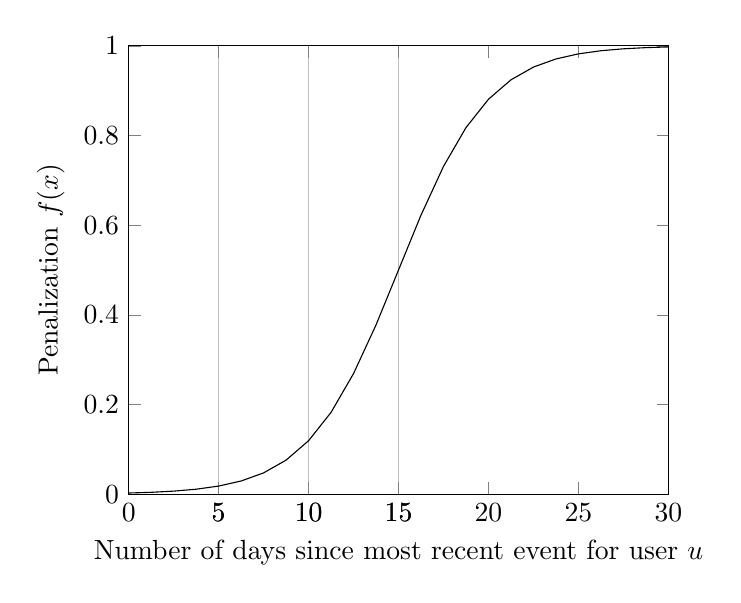
\begin{tikzpicture}
    \begin{axis}[
      ymin=0,ymax=1,
      xmin=0,xmax=30,
      xlabel=Number of days since most recent event for user $u$,
      ylabel=Penalization $f(x)$,
      extra x ticks={5,10,15},
      extra tick style={grid=major}
    ]
    \addplot[
    black,
    xlabel=$x$,
    ylabel=$f(x)$,
    domain=0:30]
    {1/(1+exp(-0.4*(x-15)))};
    \end{axis}
  \end{tikzpicture}
\end{figure}

As one can see, an event happening 15 days after the most recent event for user
$u$ will get a penalization of $0.5$ whilst an event with $x=5$ recieves
$0.018$. 

% Following up on Table~\ref{events-example} we can calculate the
% various penalizations and final scores for each day, by taking the highest
% possible score for event $i$ and penalizing it in the following manner:
%
% \begin{equation}
%   s_{e}(x,u) = b_e - (b_e - w_e) \cdot p_{x}(u)
% \end{equation}
%
% where $p_x$ is the penalization after $x$ days. $b_e$ and $w_e$ are the best
% and worst scores achievable for event $e$, respectivly. The final score
% $s_{e}(x,u)$ is presented for each event below:

\begin{table}[H]
  \centering
  \begin{tabular}{llm{2cm}ll}
    \toprule
    Num. days ($x$) & Event types & Penalization $p_{x}(u)$ & Scores & Highest score \\
    \midrule
    5   & 1,2,3 & 0.018   & 59.1, 79.64, 99.64 & \textbf{99.64} \\
    10  & 1     & 0.1192  & 55.23              & 55.23  \\
    15  & 1,2   & 0.5     & 50.0, 70.0         & 70.0 \\
    \bottomrule
  \end{tabular}
  \caption[]{}
  \label{events-example}
\end{table}
\marginpar{Perhaps represent this differently?}

When selecting a score for user $u$ we select the highest valued one, in this
case 99.64. In fact, we can optimize our algorithm by starting at the most
recent events and not calculating scores for events types that yield a lower
score than the current highest score. In the scenario above we could take all
events on $x=5$, then taken the event type with highest maximum value (3) and
ignored all other events. Note that this is only true if you have
non-overlapping event type scores/intervals, as we have per
Table~\ref{implicit-example-scores}. We can now normalize $s$ and get a rating
$r$ between $a$ and $b$ by using the following equation, knowing that $X_{max}
= 100$ and $X_{min} = 0$:
%
% \begin{equation}
%   X' = a + \frac{(X-X_{min})\cdot(b-a)}{X_{max}-X_{min}}
%   \label{eq-normalization}
% \end{equation}

Setting $a$ to 0 and $b$ to 5, as is common in recommender systems we get the
rating $X' = 4.982$ when $s = 99.64$. Intuitivly this makes sense, if we assume
event type 3 to be the highest valued event in our system it would be
equivalaent to a user buying a product - or similar. Thus, if user $u$ bought
product $i$ only $5$ days ago this would get $4.98$ as final rating. If the
user does not interact with the product again in 30 days we can re-calculate
the score, now using $x=35$ which yields a penalization of $0.999$ and score $s
= 100-((100-80)*0,999) = 80.2$, normalized in the same likert scale as above we
get a new normalized rating $4.01$ - thus still a high rating, but not as
relevant for the user as 30 days earlier.

\subsection{Considering ordering of events}

In the our previous method using the number of days since the most recent event
we encounter several weaknesses when a user is either very active or have
events with a high degree of sparsity. In the latter a user interacting with
products every 20th day would see a divide in ratings since old events are
placed after at the top of the S-curve ($f(x) > 0.9$) and new events achieves a
penalization in the lower values ($f(x) < 0.1$). Similarily, when the user is
highly active we obtain a large number of items having the same penalization
weights and in essence a large duplication of ratings, provided the spread of
event types are not large, which in many systems are unlikely. One possibility
would be to use a finer granularity on the x values, such as seconds or minutes
since the most recent event, but instead we extend our method by not taking
into consideration the \textit{time}, but instead the \textit{ordering} of
events.

As before we use an example event log where we have 10 events of three
different types (1,2 and 3) on 6 different item IDs (1001-1006).

\begin{table}
  \centering
  \label{event-log-sigmoid-count}
  \begin{tabular}{lll}
    \toprule
    Ordering & Event type & Item id \\
    \midrule
    0 & 1 & 1001 \\
    1 & 1 & 1003 \\
    2 & 3 & 1002 \\
    3 & 1 & 1004 \\
    4 & 2 & 1002 \\
    5 & 2 & 1006 \\
    6 & 1 & 1005 \\
    7 & 1 & 1001 \\
    8 & 3 & 1005 \\
    9 & 1 & 1003 \\
    \bottomrule
  \end{tabular}
\end{table}

We want to continue using the sigmoid function, but in this case we will
differentiate based on how many events we observe for a user. Further, if a
user has e.g. more than 100 events in the event log we have two options: we can
set a ceiling, saying that events older than a threshold recieves the maximum
penalty or we can distribute all items evenly and extend the max-value of
x-axis. Probably one would want a combination of the two, having a pretty large
threshold and evenly distribute the items. In the case of evenly distribute the
values you would need a \textit{distribution factor} $f$ expressing the
relationship between steepness and shift coefficients. We use the following
equation where $c$ is the number of events for user $u$.

\begin{equation}
  f_{u}(x, c) =
    \begin{cases}
      1               & \text{if } c > 1000 \\
      \frac{1}{1+e^{-(f/c) \cdot (x - c)}} & \text{else }
    \end{cases}
\end{equation}

\subsection{Linearly blending the results}

\marginpar{Move this introduction to the pre-study?}
At this point we have found multiple novel ways of calculating the
implicit ratings, based on our implicit feedback. However, as one may observe
each method has its weknesses and strengths. A sigmoid-function considering the
number of days between events is good for including our implicit knowledge
about seasons into the ratings, but is not as effective if users has high
spread in between events or low activity. Further, there may exist some clothes
that has longer life-span than others, e.g. warm jackets that generally are
bought from September to March (7 months) compared to shorts which are
generally bought from May to August (4 months), depending on where the store
reside. Our second sigmoid function has the strength of always keeping the
ratings for a user fresh, also for less active users, but it is weaker in
differentiating between seasons - which can be seen if a user is on a hiatus
between January and August, not using the application. Upon return all ratings
would be based on his/hers winter activity, not penalizing the fact that the
type of clothes generally bought in the store at this time are different than
in January.

Optimally we would like to combine these two methods, taking their strenghts
and weaknesses together trying to average them out in order to end up with
generally better ratings - where we cannot trivally imagine scenarios as
depicted above where our models would fail. The process of combining such
ratings are in the Recommender Systems community called \textbf{blending} and
is in many ways a seperate research area in itself, if done advanced enough.
However, in the case of the naive and linear blend on can achieve results a
magninute higher than for each method seperatly as seen in \ref{}
\marginpar{find some refs using linear blending}.

When linearly blending $M$ models $m$, we choose $M$ factors $f$ all adding up
to 1.0, representing the weight of model $m_{i}$ in the final blend. Then when
calculating the final rating for item $j$ we sum over all models:

\begin{equation}
  r_j = \sum _{i=1}^{M} f_{i} * m_{j}
\end{equation}

As one may observe given the linear blend between with factors $f_1 = 0.7$ and
$f_2 = 0.3$ and the two ratings $m_1 = 5$ and $m_2 = 3$ for a given item, we
can calculate the final rating as $0.7 \cdot 5 + 0.3 \cdot 3 = 4.4$. A weakness
when linearly blending models in this way is the need for manually finding good
weights for the $M$ factors. There exists methods where this given a good test
set can be done automatically, such as using Linear Regression or KNN blending.
Many other blending schemes exists as well, such as Binned Linear Regression,
Bagged Gradient Boosted Decision Tree (BGBDT), Neural Networks and Kernel Ridge
Regression Blending \cite{jahrer2010combining} \cite{toscher2009bigchaos}.

As we have multiple proposed models we present our results given various
evaluation metrics and combinations of weights. Note that when a model has the
weight 1.0 its equal to that the model has not been blended with any other
model, and is included in the table below as a baseline.

\begin{table}[H]
  \centering
  \begin{tabular}{lll|ll}
    \toprule
    \textbf{Naive} &  \textbf{Sigmoid Count} & \textbf{Sigmoid Recent} &
    \textbf{RMSE} & \textbf{MAE} \\
    \midrule
    1.0  &      0.0        &      0.0       &  X   &  X  \\
    0.0  &      1.0        &      0.0       &  X   &  X  \\
    0.0  &      0.0        &      1.0       &  X   &  X  \\
    \midrule
    0.6  &      0.2        &      0.2       &  X   &  X  \\
    0.5  &      0.3        &      0.2       &  X   &  X  \\
    0.4  &      0.3        &      0.3       &  X   &  X  \\
    0.3  &      0.3        &      0.4       &  X   &  X  \\
    0.2  &      0.4        &      0.4       &  X   &  X  \\
    0.1  &      0.4        &      0.5       &  X   &  X  \\
    0.0  &      0.5        &      0.5       &  X   &  X  \\
    \bottomrule
  \end{tabular}
\end{table}

As one may see, the best results are achivied when blending with...
\marginpar{todo: analyze and finish this table}

% !TEX root = ../../report.tex
\clearpage
\section{Experimental Plan}

%We can sometimes evaluate how well the recommender achieves its overall goals.
%For example, we can check an e-commerce website revenue with and without the
%recommender system and thereby estimate the value of the system to the website.

Section \ref{evaluation} covers a wide range of evaluation metrics that
measure different properties of the recommender system. This section will cover
our experimental plan, starting off by looking at the goals for our experiments.
The remaining parts of the section will describe the datasets used for evaluation,
our evaluation methodology and our evaluation metrics of choice.
The section will also describe the datasets used for evaluation, our evaluation methodology

We have the following goals for our experiment:

\begin{itemize}
	\item Does our proposed implicit rating methods improve the recommendation quality over
	binary preference data?
	\item Compare the different implicit rating functions.
	\item Select the best combination of methods for the SoBazar recommender system.
\end{itemize}

\marginpar{Supervisors: Any suggestions?}
\marginpar{TODO: Discussion on how}

Then the question is, how can we determine whether a method is better than another. The
main reasons for implementing a recommender system is the desire to improve user
satisfaction and to increase the economic success of a platform. Although both goals
are interrelated they may be competing in some scenarios. The user might be more interested
in purchasing the products with the best price-performance ratio, while the \emph{owners}
are more interested in showing the products that lead to the highest revenue for the
business. For this purpose, a commercial recommender could/should consider implementing
a reward attribute for items that show how much the company profits from its sale. This
information can then e.g. be used in a combination the recommendation list of the recommender
to produce the final recommendations.

\begin{figure}[H]
		\centering
	  	\includegraphics[height=0.65\linewidth]{image/evaluationpipeline.png}
		\caption[A Traditional Evaluation Pipeline]{A traditional evaluation pipeline for evaluating recommender systems}
		\label{figure:evaluationpipeline}
\end{figure}

In order to further specify our goals we therefore have to take a closer look at the recommender's task,
its interface and the available data. The most typical task for a e-commerce recommender system is to determine an order of items, often with the purpose of creating a top-k list of items that is shown in a sidebar or on a
dedicated page.

\begin{figure}[H]
		\centering
		\begin{minipage}{.45\linewidth}
	  		\includegraphics[height=1.2\linewidth]{image/sobazarfeed2.png}
		\end{minipage}
		\begin{minipage}{.45\linewidth}
			\includegraphics[height=1.2\linewidth]{image/sobazarsale.png} 
		\end{minipage}
		\caption[Sobazar news feed - version 0.5.1]{Sobazar news feed}
		\label{figure:sobazarfeed}
\end{figure}


The above figure shows the Sobazar feed. Recommendations are likely to be shown in a similar fashion, but instead as \emph{recommended for you}. The interface currently let you scroll sideways over up to 20 items.

Ultimately, the goal of the experiment is to evaluate and measure the properties
of the system, which we have identified as the most important for the systems success,
and select the method that performs the best overall with respect to these properties.

\subsection{Selecting datasets for evaluation}

In addition to evaluate the methods on the Sobazar dataset we want to make sure that our
solution generalizes beyond our experimental dataset, in accordance to the general guidelines
for experimental studies \cite{Shani2011}. The data used for offline evaluation should match
as closely as possible the data we expect the recommender system to face when it is
deployed \cite{Gunawardana2009}. When selecting datasets for evaluation we focused on the
following dataset properties:

\begin{itemize}
	\item Size of dataset: Preferable as close as possible to Sobazar (6 months from now)
	in terms of number of ratings, users and items.
	\item Different types of user feedback: Preferable different types of implicit feedback
	such as browsing and buying behavior.
	\item Domain: Preferably a domain as close to possible as the e-commerce domain with respect
	to the importance of factors such as recentness.
	\item Presence of features: To evaluate the hybrid methods.
	\item Timestamps: To evaluate the recentness mapping
\end{itemize}

We were unable to acquire any e-commerce datasets containing user browsing history, purchases etc.
And we therefore had to turn for other domains for datasets...

%The first dataset we chose for evaluation was the MovieLens 1M dataset. The reason for selecting the MovieLens 1M dataset over MovieLens 100K is that the number of users is closer to what we expect the SoBazar to have after the \emph{official} launch this summer in addition to having user- and item features. The MovieLens dataset can also be seen as a \emph{benchmark} dataset as it is one of the most popular recommender systems dataset used for evaluation in countless articles.

\subsubsection{Book-Crossing Dataset?}

Use implicit feedback as \emph{item-clicked} and explicit ratings greater than 5 as \emph{item-liked}.

\subsection{Simulating user behavior?}

%General statistics and averages
%Interesting findings/properties
%Was cleaning neccesary?
%How was the methods evaluated on the dataset?
%	- x-fold cross validation


%\subsubsection{MovieLens 1M}
%
%As our second dataset we have chosen the MovieLens 1M dataset. The dataset contain 1,000,209 anonymous ratings on approximately 3,706 movies (The readme mentions 3900 movies) made by 6040 users. User features included age, gender, occupation and zipcode, item features include movie genre. Each user included in the dataset have provided a minimum of 20 ratings. The average rating given to movies in the dataset is $3.58$. There are 18 different genres in the dataset, but each movie can have multiple genres assigned to it, of which there are 498 different combinations in the dataset.
%
%\begin{table}[H]
%\centering
%\begin{tabular}{|l|l|}
%\hline
%Male & Female \\ \hline
%4331 & 1709 \\ \hline
%\end{tabular}
%\caption{MovieLens Gender Distribution}
%\end{table}
%
%\begin{table}[H]
%\centering
%\begin{tabular}{|l|l|l|l|l|l|l|}
%\hline
%Under 18 & 18-24 & 25-34 	& 35-44 	& 45-49 & 50-55 & 56+ \\ \hline
%222		 &	1103 &	2096	&	1193	& 550	& 496	& 380 \\ \hline
%\end{tabular}
%\caption{MovieLens 1M Age Group Distribution}
%\end{table}
%
%\begin{table}[H]
%\centering
%\begin{tabular}{|l|l|}
%\hline
%Other/not specified  & 711  \\ \hline
%Academic/Educator  & 528  \\ \hline
%Artist  & 267 \\ \hline
%Clerical/Admin & 173 \\ \hline
%College/Grad student  & 759 \\ \hline
%Customer service & 112 \\ \hline
%Doctor/Health care & 236 \\ \hline
%Executive/Managerial & 679 \\ \hline
%Farmer & 17 \\ \hline
%Homemaker & 92 \\ \hline
%K-12 student & 195 \\ \hline
%Lawyer & 129 \\ \hline
%Programmer & 388 \\ \hline
%Retired & 142 \\ \hline
%Sales/Marketing & 302 \\ \hline
%Scientist & 144 \\ \hline
%Self-employed & 241 \\ \hline
%Technician/Engineer & 502 \\ \hline
%Tradesman/Craftsman & 70 \\ \hline
%Unemployed & 72 \\ \hline
%Writer & 281 \\ \hline
%\end{tabular}
%\caption{MovieLens 1M Occupation Distribution}
%\end{table}
%
%As the sparsity of this dataset is fairly low (95.53164), we decided to evaluate this dataset using the holdout method. As the dataset include time-stamps we split the dataset based on time, meaning that all ratings given before a given time will be used to train the model and all ratings given after this point will be used as a testset. We set aside the last 25\% ratings for evaluation and train the model using the remaining 75\%.

\subsubsection{The Sobazar Dataset}

The Sobazar dataset is smallest and sparsest of our datasets used for evaluation.
The dataset contain ratings 15,252 given by 1,235 users to 3,386 items.
We also have access to semi-structured product information collected/crawled from
the online retailers for \emph{some} items. In addition user data from the users
can also be downloaded from Facebook.

Having such a small and sparse dataset has several implications. Firstly we have
to avoid \emph{wishful thinking} as we have very thin data, meaning that we cannot
rely on getting reliable results. Secondly, our evaluation methodology must be
\emph{tailored} for small sparse datasets. When using cross-validation the number
of folds depends on the size of the dataset. For large datasets, even 3-fold Cross
Validation will be quite accurate, while for very sparse datasets, we may have to
use leave-one-out in order to train on as many examples as possible. The advantages
of using a large number of folds is that the bias of the true error rate estimators
will be small (the estimator will be very accurate), with the disadvantages being that
the variance of the true error rate estimator will be large in addition to increased
computation time. To exemplify this we ran a small experiment on the Sobazar data using
IBCF, with $k-NN=3$, experimenting with different $K$-fold values:

\begin{table}[H]
\centering
\begin{tabular}{l l l l l }
\toprule
K-fold & 	$min_{RMSE}$ 	&	$max_{RMSE}$ 	& Average 	& Variance 					\\ \midrule
3	   & 	0.783 			& 	0.789 			& 0.785 	& $8.730 \times 10^{-6}$	\\ 
5	   & 	0.759			& 	0.802 			& 0.781 	& $3.363 \times 10^{-4}$ 	\\ 
8	   & 	0.740			& 	0.781			& 0.758 	& $1.656 \times 10^{-4}$ 	\\ 
10	   & 	0.718 			& 	1.026			& 0.810  	& 0.0125					\\
\bottomrule
\end{tabular}
\caption{Evaluation results from experimenting with different k-fold splits on the Sobazar dataset}
\end{table}

\marginpar{TODO: This table is not really necessary to include...}

When increasing the number of folds we could see that it was unable to generate
any recommendations at all for some folds, or getting really poor results, meaning
that we get some difficult splits. E.g. when using 30 folds, IBCF was unable to
provide any recommendations for 8 folds out of 30. By using more than 10 folds
it is increasingly likely that we end up with a few or more \emph{unrecommendable}
instances in the test set, yielding no test result. Based on these results,
and the general consensus that more folds are better for small datasets we
believe that using between $5-10$-folds would be a good choice for model validation.
Another alternative well suited for sparse datasets is the \emph{all but one} or the
\emph{leave one out} method, in which we remove one rating from the test users
and try to predict the hidden rating.

Another important concern is whether or not to take the timestamps into consideration,
which directly speaks against the use of cross-validation, as we wish to use the past
interactions to predict future actions. When using the \emph{leave one out} method one
could e.g. select a predetermined set of test users based on some criteria and remove
their latest rating and try to predict it and repeat the process any number of times.
This is particularly relevance as our implicit mapping function takes recency into account.


\subsubsection{Overview of the Datasets}

Table \ref{table:datasets} shows an overview of the datasets used for evaluation.

%TODO - What else is interesting to know? Rating scale, average number of ratings per user, number of cold start users...
%TODO - % of users with less than 5 ratings for both datasets

\begin{table}[H]
    \centering
    \begin{tabular}{l l l l l l }
    \toprule
	Dataset			& 	Ratings 	& 	Users	& 	Items 	& 	Sparsity	& Rating Scale 				\\ \midrule
	Sobazar 		& 	27,873  	& 	1,511	&	5855	&	99.69657	& Implicit Ratings(1-5)		\\ 
	%Movielens 1M	& 	1,000,029   &	6040 	&	3706	&	95.53164	& Explicit (1-5)			\\ 
	Dataset 2 		& 	-  			& 	-		&	-		&	-			&							\\
	\bottomrule
    \end{tabular}
    \caption [Overview of the datasets used for evaluation]{Overview of the datasets used for evaluation}
    \label{table:datasets}
\end{table}

\subsection{Simulating the Cold-Start Problem}

To simulate the cold-start problem and evaluate how well our the different
methods tackle the different cold-start situations we used the following
evaluation methodology. As mentioned in Section \ref{sec:cold-start-eval} there is
no common framework for assessing the cold-start performance of recommender systems.
Our goal is to come up with \emph{comprehensive} framework to assess the cold-start
performance of our recommender systems. The following inputs changes the dataset over time:

\begin{itemize}
	\item 	Existing users watch new items in the catalogue
	\item	New users join the system and view their first item
	\item	New items are added to the catalogue
\end{itemize}

The first input source has the effect of increasing the dataset density, the average user
profile length, and the average number of views per item. The second input factor has
the effect of decreasing both the dataset density and the average user profile length,
as the new users that join the system have interacted with only a few items. Similarly, the third input
factor has the effect of decreasing both the dataset density and the average number of
views per item.

To simulate the cold-start user problem we propose splitting the users into two disjoint
sets, similarly as in \cite{Stern2009, Lam2008}, using 90\% of the users for training and
setting aside the remaining 10\% for evaluation. We then train the model with e.g. 5, 15,
25 and 35 ratings and predict the remaining values. Alternatively one could train the model
using e.g. 25\% and 75\% of each test users ratings. Similarly, to simulate the cold-start
item problem we again split the items into two disjoint sets, using 90\% of the items
for training and the remaining 10\% for evaluation.  We then train the model with
e.g. 20, 40, 60 and 80 ratings and predict the remaining values. The selection criteria
for test items and users can differ from dataset to dataset. E.g. in \cite{Rashid2002, Rashid2008}
the authors selected a subset of the users with more than 200 ratings, but you can not
expect 10\% all the users for all datasets to have provided 200 ratings, so this number
might be lowered if necessary. The implications of removing the top 10\% of the
raters from the Sobazar dataset is fairly large as they stand for a large portion
of the few ratings we have.

To evaluate the cold-start system performance we use the same method as described
in ~\cite{Agarwal2009} where the authors propose using a 75:25 training/test split,
where we at random draw e.g. 35\%, 50\% and then finally use all (75\%) of the
ratings in the training set and predict the remaining 25\%.

\marginpar{TODO: Add some justification...}

%TODO - How is this implemented on the sobazar data?

For the Sobazar dataset we select 10\% of the users as test users, for a user to be
selected as a test user, the user must have provided at least 20 ratings. The test user are drawn
at random from the eligible candidates. We then train
the model using 10\%, 40\% and 75\% of their ratings and try to predict their remaining ratings.
The reason for choosing percentages over hard limits is due to the fact that the ratings are
distributed unevenly among the users. As we have a very low number of ratings and a large item collection we had to use
only 5\% of the items as test items, where each test item have been rated by atleast 15 users.
We train the model using 10\%, 40\% and 75\% of their ratings and try to predict their remaining
ratings. As we have access time timestamps, we split the users and items based on timestamp.
E.g. for the 10\% user split we train the model with their initial ratings and try to predict
their following ratings. To evaluate the cold-start system performance we split the dataset in a test
and training set using 20\% of the ratings for testing and then train the model
using 40\%, 60\% and 80\% of the ratings for training. It is important to note that
this process should be repeated multiple times, as the chance of getting an
\emph{unfortunate} split is highly probable due to the dataset size. For the cold-start
system task we also split the dataset based on timestamps, meaning that the test set consists
of the most recent ratings.

%TODO - How is this implemented on the x dataset?


\subsection{Evaluation Metrics}

%TODO - Discussion of evaluation metrics

%http://www.slideshare.net/gunnar-schroeder

A large variety of metrics have been published, and some of these metrics are highly correlated \cite{Herlocker2004}.
There is little guidance for evaluating recommender systems and choosing metrics. However, there are
some important questions one should ask oneself when selecting evaluation metrics:

\begin{itemize}
	\item Which aspects of the usage scenario and the data influence the choice?
	\item Which metrics are applicable?
	\item What does these metrics express?
	\item What are the differences among them?
	\item Which metric represent our user-case best?
	\item How much do the metrics suffer biases?
\end{itemize}

It is safe to assume that the users are more interested in the top ranked items, than rating
predictions for the entire item collection. Evaluation of top-k recommendations suggests a
classification or ranking task, evaluation should therefore focus on classification or ranking metrics.

\begin{figure}[H]
  \centering
  \includegraphics[height=.5\linewidth]{image/sobazarmostpop.png}
  \caption[Sobazar most-popular recommendation]{The Figure shows how the most-popular recommendations are shown in the application}
\label{figure:mostpopular}
\end{figure}

Much like the social feed shown in Figure \ref{figure:sobazarfeed} up to 20 popular items can be shown.
It would also be beneficial to rank these recommendations putting the most popular/relevant items in the first 4 slots and sorting the remaining items in descending order based on popularity. This implicates that a metric that measures the overall ranking is not appropriate, and that we only should measure the ranking quality of the $k$ items being shown, the other items are irrelevant. The above reasoning lead us to take a closer look at classification and ranking accuracy metrics.

%TODO - Add some more cites

The area under curve (AUC) is a popular classification accuracy metric. ROC curves provide a graphical
representation for the performance of a recommender system, by plotting the recall (True positive rate)
against the fallout (False positive rate) for increasing recommendation set size. A perfect recommender
would therefore yield a ROC curve that goes straight up towards 1.0 recall and 0.0 fallout until all
relevant items are retrieved. Afterwards it would go straight towards 1.0 fallout while the remaining
irrelevant items follow. One therefore obviously aims to maximize the area under the curve (AUC). The higher
up all relevant items (True positives) are in the recommendation list, the higher the AUC score will be.
AUC can therefore be used as a single measure for the overall quality of a recommender system. Table \ref{table:auc}
shows an example of the AUC values when varying the position of a single relevant document through the
recommendation list.

\begin{table}[H]
	\centering
	\begin{tabular}{*{12}l}
	\toprule
	\#Example	& R1 & R2 & R3 & R4 & R5 & R6 & R7 & R8 & R9 & R10 & AUC \\ \midrule
	1		& \cmark & \xmark & \xmark & \xmark & \xmark & \xmark & \xmark & \xmark & \xmark & \xmark & 1.000 \\ 
	2		& \xmark & \cmark & \xmark & \xmark & \xmark & \xmark & \xmark & \xmark & \xmark & \xmark & 0.889 \\ 
	3		& \xmark & \xmark & \cmark & \xmark & \xmark & \xmark & \xmark & \xmark & \xmark & \xmark & 0.778 \\ 
	4		& \xmark & \xmark & \xmark & \cmark & \xmark & \xmark & \xmark & \xmark & \xmark & \xmark & 0.667 \\ 
	5		& \xmark & \xmark & \xmark & \xmark & \cmark & \xmark & \xmark & \xmark & \xmark & \xmark & 0.556 \\ 
	6		& \xmark & \xmark & \xmark & \xmark & \xmark & \cmark & \xmark & \xmark & \xmark & \xmark & 0.444 \\ 
	7		& \xmark & \xmark & \xmark & \xmark & \xmark & \xmark & \cmark & \xmark & \xmark & \xmark & 0.333 \\ 
	8		& \xmark & \xmark & \xmark & \xmark & \xmark & \xmark & \xmark & \cmark & \xmark & \xmark & 0.222 \\ 
	9		& \xmark & \xmark & \xmark & \xmark & \xmark & \xmark & \xmark & \xmark & \cmark & \xmark & 0.111 \\ 
	10		& \xmark & \xmark & \xmark & \xmark & \xmark & \xmark & \xmark & \xmark & \xmark & \cmark & 0.000 \\
	\bottomrule
	\end{tabular}
	\caption{Varying the position of a single relevant item on a four out of ten recommendation list}
	\label{table:auc}
\end{table}

One should also be aware of that the AUC scores can be highly inaccurate, especially for cold-start users,
users which the recommender is unable to provide more than a handful of recommendations for. This is
due to the fact that all unknown ratings are appended in random order after the known recommendations.
E.g. lets say the recommender is able to generate 10 recommendations for a user out of 4000 items,
and that one out of two test items for that user is not in the recommended list from the recommender.
Where the last test item is appended in the recommendation list can mean the difference between a AUC score of above
0.9 to less than 0.6 if the item is appended at the end of the list, the results can be even more
severe if none of the items is in the initial recommended list, then the results for that user will be completely random. The most obvious solution to this problem would be to use resampling or to repeat
the experiment multiple times where the items not in the recommendation list are drawn at random and
the results averaged over all the trials.

However, a frequently uttered point of criticism is that users are often more interested in the items
at the top of a recommendation list but that the AUC measure is equally affected by swaps at the top
or the bottom. To \emph{complement} AUC, we also wish to measure the rank accuracy, to get a better
overall picture of the systems performance. This means that we want to measure whether or not
highly rated items such as purchases, likes etc. are ranked higher than less relevant items such as clicks,
as having these highly ranked items higher up in the recommendation list aligns with our previously
mentioned financial incentives.

%TODO - What is the "best" rank-accuracy metric?

When using rank accuracy metrics, it is worth knowing whether one is measuring total or partial orderings.
Most rank accuracy metrics (e.g. Kendall's tau and Spearman's rho) compare two total ordering. The problem
with these measures is that we in most cases are not provided with a full ranking of the items as most recommendation
algorithms only generate a partial list of items that are likely to be preferred by a user. The remaining items
would therefore have to be concatenated in random order. The recommendation list can also consist of several
items with similar rating that can appear in varying orders. Therefore, in order to create a full ranking of
the items all preference values for the user have to be known. Since the user can express the same rating for similar
items, the list will again contain groups of items that can appear in arbitrary order. However, the largest problem
is posed by items for which no rating is known. These items could hold an arbitrary place within the ranking.
Again, consider an example where a user e.g. have rated 5 items out of 4000, and the recommender is able to recommend
only 10 items for that user. To measure the rank accuracy we would have to randomly add 3995 items to the users known
preference list and 3990 to the users prediction list. Comparing the order of these lists would not make much sense. The bottom line is that in most cases a rank metric for partial ordering would be more appropriate for comparing recommendation lists that are produced by recommenders to item rankings from known user preferences.

We assume that we can recommend at most $k$ items for each user at a time. It also pays to submit all $k$
recommendations, because we are not penalized for bad guesses. We also assume that the order matters, so it
is better to submit more certain recommendations first, followed by recommendations we are less sure about.
Which means that we basically select the $k$ best candidates in order. To reduce the number of randomness in
the results one could choose to only look at the ranking of the top $k$. However, the problem is that the
likeliness of finding a \emph{hidden} item in e.g. the top 20 recommended items is not very large when one is working
with large item catalogs. The problem then, is how to select the value of $k$. Setting it to low you risk
ending up with many $0.0$ values, and when setting it to high you risk including to many \emph{randomly} concatenated 
ratings in the results.

%MyMediaLite Problems
%	Very few 'remaning items' are appended with a rating of 0.0, how do we determine a cutoff point?

%How certain are we about the order? (Do we look at rank? How much weight should be given...?)

Mean average precision (MAP@k), described in Section \ref{subp:mean_average_precision_map_} is a popular metric for search engines and is applied, for example, to report results at the Text Retrieval Conference (TREC). The main weakness with regard to recommender systems is that it assumes that the user is interested in finding many relevant documents for each query, and does not look at the relevance of the items. Consider the following examples where we have three lists of hidden items and three recommendations lists. All none relevant items are labeled with the item-id $0$.

\begin{table}[H]
\label{table:ap}
\centering
\begin{tabular}{*{4}l}
\toprule
Example 	& 	Actual	& 	Recommended		&	AP@4   \\ \midrule
1			& [1,2,3,4]	&	[1,0,0,0]		&	0.250  \\ 
2			& [1,2,3,4]	&	[2,0,0,0]		&	0.250  \\ 
3			& [1,2,3,4]	&	[3,0,0,0]		&	0.250  \\
\bottomrule
\end{tabular}
\caption{AP@4 Scores}
\end{table}

As you can average precision does not consider the order of the actual item list. We want a way to
reward the recommender for getting the highly ranked items right.

Normalized Discounted Cumulative Gain ($nDCG_{k}$), described in Section \ref{subp:normalized_discounted_cumulative_gain_}
is another metric to measure the rank accuracy. It is based on two main assumptions; (1) Highly relevant items are more useful than marginally relevant ones, (2) The lower the ranked position of a relevant item, the less useful it is for the user, since it is less likely to be \emph{examined}. The maybe most interesting aspect of nDCG is that it contains an utility function $rel_i$. One can replace the original utility function and replace it with a function that is more relevant to the application. Two such examples include:

\begin{itemize}
\item $rel_i = 1/log(i+k)$, where i is the index of the item in the actual sorted rating list, where $k$ is a constant.
\item $rel_i = u(i)$, simply assign the rating of an item as its relevance.
\end{itemize}

For our application we believe it to be beneficial to use the rating of the item as a
relevance score, as we could have multiple items with highly similar ratings (thus the same relevance). When using a low $k$ value for the logarithmic alternative this could mean that the relevance between two almost similarly rated items might end up being disproportionately large. We will also most likely look at the 20 top items, which means that the difference between the lower ranked items will be fairly small, as the logarithmic function converges. A third alternative would be to also use some linear decay function. The following table shows the $nDCG$ score for a set of examples where the function $rel_i = 1/log(i+1)$ is used to assign the relevance score to item $i$ in the sorted list of actual ratings. E.g. item one is assigned a relevance score of $1/(log(2)$ and so on. We hope the following table will give the reader a better idea of how $nDCG$ \emph{works}.

\begin{table}[H]
\label{table:ndcg}
\centering
\begin{tabular}{*{4}l}
\toprule
Example 	& 	Actual					& 	Recommended				&	nDCG 	\\ \midrule
1			& 	[1,2,3,4]				&	[1,0,0,0]				&	0.470   \\ 
2			& 	[1,2,3,4]				&	[2,0,0,0]				&	0.360   \\ 
3			& 	[1,2,3,4]				&	[3,0,0,0]				&	0.330   \\ 
4			& 	[1,2,3,4,5,6,7,8,9,10] 	& 	[1,2,3,4,5,6,7,8,9,10] 	&   1.000	\\ 
5			& 	[1,2,3,4,5,6,7,8,9,10] 	& 	[10,9,8,7,6,5,4,3,2,1] 	&   0.900	\\ 
6			&	[1,2,3,4,5,6,7,8,9,10] 	& 	[1,2,0,0,0,0,0,0,0,0] 	&   0.440	\\ 
7			& 	[1,2,3,4,5,6,7,8,9,10] 	& 	[1,0,0,3,0,0,0,0,0,0] 	&   0.390	\\ 
8			& 	[1,2,3,4,5,6,7,8,9,10] 	& 	[4,0,0,0,8,0,0,0,0,0] 	&   0.280	\\ 
9			& 	[1,2,3,4,5,6,7,8,9,10] 	& 	[0,0,0,0,5,0,0,0,0,10] 	&   0.130	\\ 
10			& 	[1,2,3,4,5,6,7,8,9,10] 	& 	[0,0,0,0,0,0,0,0,9,10]	&   0.110	\\
\bottomrule
\end{tabular}
\caption{nDCG Test Examples}
\end{table}

As you can see from the above mentioned examples nDCG will give us an indication whether or not our recommender
ranks \emph{highly relevant} items above those who are less relevant. As for the limitations, nDCG is designed for situations of non-binary notions of relevance, thus it cannot be used in our experiment where we wish to compare binary ratings with implicit ratings. The main difficulty encountered in using nDCG is the unavailability of an ideal ordering of results when only partial relevance feedback is available. This is often the case when we have several equally good results. This is especially true when the metric is limited to only first few results as it is often done in practice.

We chose take a closer look at the different ways of calculating nDCG. There are two commonly used methods used to calculate the DCG and IDCG scores.

\begin{itemize}
\item Method 1  $DCG_p = rel_1 + \sum_{i=2}^{p} \frac{rel_i}{log_2(i)}$
\item Method 2: $DCG_p = \sum_{i=1}^{p} \frac{2^{rel_i}-1}{log_2(i+1})$
\end{itemize}

The following table shows the differences between Method 1 and Method 2 on a few selected examples. Here we set the value of $rel_i$ equal to the implicit rating of item $i$.

\begin{table}[H]
\label{table:ndcgfinal}
\centering
\begin{tabular}{*{5}l}
\toprule
\#Ex & 	Actual																	& 	Recommended				&	$nDCG^1$  	   & $nDCG^2$	\\ \midrule
1 		& 	[$1_{5}, 2_{3.8}, 3_{3.55}, 4_{2.78},5_{1.3}$]								&	[5,0,0,0,0]				&	0.113 		   & 0.026  \\ 
2 		& 	[$1_{5}, 2_{3.8}, 3_{3.55}, 4_{2.78},5_{1.3}$]								&	[0,0,1,0,0]				&	0.217 		   & 0.275   \\ 
3   	& 	[$1_{5},2_{4.8}, 3_{3.55}, 4_{2.78}, 5_{2.2}, 6_{2.0},7_{1.77},8_{1.3}$]		&	[2,3,4,5,6,7,8,0]		&	0.827		   & 0.682   \\ 
4  		& 	[$1_{5},2_{4.8}, 3_{3.55}, 4_{2.78}, 5_{2.2}, 6_{2.0},7_{1.77},8_{1.3}$]		&	[1,2,0,0,0,0,0,0]		&	0.592 		   & 0.805   \\
5 		& 	[$1_{5},2_{4.93},3_{2.88}, 4_{1.85},5_{1.8},6_{1.77}, 7_{1.63},8_{1.52}$]	&	[1,0,0,0,0,0,0,0]		&	0.394 		   & 0.544   \\
6 		& 	[$1_{5},2_{4.93},3_{2.88}, 4_{1.85},5_{1.8},6_{1.77}, 7_{1.63},8_{1.52}$]	&	[3,4,5,6,7,8,0,0]		&	0.542 		   & 0.206   \\
\bottomrule
\end{tabular}
\caption{Comparison of nDCG scores for different methods of computing DCG. Each item in the Actual list is on the form $ItemId_{Rating}$, the first item in the actual list of example one therefore has en ItemId of 1 and a Rating of 5. All non relevant items are given the ItemId 0 in the Recommended list.}
\end{table}

As you can see Method 1 is a bit more \emph{balanced} than Method 2, as it does not give as much weight to highly rated items. Especially example 5 and 6 highlights this as Method 2 prefers retrieving one highly rated item over retrieving multiple less relevant ones. Method 2 is ultimately closer to what we want in addition to being commonly used by web search companies and on the data science competition platform Kaggle \cite{kaggle}. We have also chosen to truncate the recommendation list and only calculate the nDCG of the $k$ top items. Because nDCG has a relatively low positional discount, it allows us to set $k$ fairly high, but this only makes sense if we believe that the user will read large portions of the recommendation list. 

\marginpar{TODO: Spend any more time looking at partial order ranking measures?...}

%TODO - Select K value based on user interface
%TODO - Justify why these metrics combined will give a good overview of the performance.
%TODO - Cold-start evaluation Metrics

In addition to looking at the above mentioned metrics it would be interesting to see how
the different sparsity levels affect both the user- and item-space coverage of the different
methods when evaluating the cold-start system performance, as having a recommender that can only
recommend a limited set of items to a small portion of the users is \emph{unfortunate}. The
user-space coverage is the number of users the recommender is able to produce recommendations for while the item-space
coverage is measured by looking at how many of the items are recommendable.

%TODO - How will these experiment be carried out and validated?

\subsection{Comparing ratings}

Figure \ref{implicitRatingEvaluation} shows the process of evaluating a set of generated ratings. The \emph{million dollar question} is: how to do we evaluate a set of ratings?

\begin{figure}[H]
		\centering
	  	\includegraphics[height=0.65\linewidth]{image/ratinggeneval.png}
		\caption[Comparing Ratings]{The Figure shows the process of comparing ratings}
		\label{figure:compareratings}
\end{figure}

Evaluating and comparing a set of ratings is not something you often encounter in the literature.
\marginpar{TODO: Are there any articles on something similar?}
We have a few initial theories of how it can be done:

\begin{enumerate}
\item Using the log data as the ground truth. Is it possible to justify that one method is better than another with observations from the log data?
\item Can we put the ratings into a traditional recommender system evaluation pipeline and use the results from that to compare the ratings. In that case, what evaluation metrics are suitable?
\end{enumerate}

The bottom line is that evaluating the quality of a set of generated ratings is hard. 



We could say that we believe that better ratings gives us better recommendation results, and use this as a basis for our evaluation. However, this means that the results we get from testing the different algorithms with different rating sets should be comparable. The problem with this is that most evaluation metrics consider the supplied ratings as the ground truth and bases its evaluation on these numbers. This automatically disqualifies any evaluation metrics that consider the rating values such as e.g. MAE.


\subsection{Implicit Ratings vs. Binary Preference}

This subsection will attempt to explain how we will attempt to determine whether our implicit gives some added
qualities in form of improved recommendations produced using binary preferences.

Problems: Methods that can incorporate both types of feedback...
Problems: Methods for implicit ratings (Explain why traditional item-based cf is not suited...)

\begin{center}
    \begin{tikzpicture}
		[node distance = 1cm, auto,font=\footnotesize,
		% STYLES
		every node/.style={node distance=1.5cm},
		% The comment style is used to describe the characteristics of each process
		comment/.style={rectangle, inner sep= 5pt, text width=3cm, node distance=0.25cm, font=\scriptsize\sffamily},
		% small comment lol
		comment-small/.style={rectangle, inner sep= 5pt, text width=1cm, node distance=0.25cm, font=\scriptsize\sffamily},
		% The nonProcess style
		nonProcess/.style={rectangle, draw, inner sep=5pt, text width=3cm, text badly centered, minimum height=1.2cm, font=\footnotesize\sffamily},
		% The process style is used to draw the processs' name
		process/.style={rectangle, draw, fill=black!10, inner sep=5pt, text width=3cm, text badly centered, minimum height=1.2cm, font=\bfseries\footnotesize\sffamily},
		% ratingsGenerator style
		ratingsGenerators/.style={rectangle, draw, fill=blue!50, inner sep=5pt, text width=3cm, text badly centered, minimum height=1.2cm, font=\bfseries\footnotesize\sffamily},
		% racommendation algorithms
		recAlgs/.style={rectangle, draw, fill=red!40, inner sep=5pt, text width=3cm, text badly centered, minimum height=1.2cm, font=\bfseries\footnotesize\sffamily}]

		% Draw processs
		\node [ratingsGenerators] (rg1) {sigmoid\_fixed};
		\node [ratingsGenerators, right=0.25 of rg1] (rg2) {sigmoid\_constant};
		\node [comment-small, right=0.01 of rg2] (dotdotdot) {..............};
		\node [ratingsGenerators, right=0.01 of dotdotdot] (rg3) {norm\_dist};

		\node [process, below of=rg2] (gt) {"Ground Truth"};

		\node [recAlgs, below of=gt] (ra2) {ALS};
		\node [recAlgs, left=0.25 of ra2] (ra1) {KNN};
		\node [comment-small, right=0.01 of ra2] (dotdotdot2) {..............};
		\node [recAlgs, right=0.01 of dotdotdot2] (ra3) {wALS};

		\node [process, below of=ra2] (eval) {Evaluation Score};

		% \node [nonProcess, below of=implicitConverter] (ratings) {Ratings for the items};
		% \node [process, below of=ratings] (recommendations) {Make recommendations};
		% \node [process, below of=recommendations] (evaluations) {Evaluate recommendations};
		% \node [nonProcess, below of=evaluations] (evaluationValue) {Recommendation score};

		%%%%%%%%%%%%%%%
		% Comments
		\node [comment, right=0.25 of rg3] (comment-rg3) {
			Implicit ratings
		};
		\node [comment, right=0.25 of ra3] (comment-ra3) {
			Recommendations algorithm
		};
		% \node [comment, right=0.25 of ratings] (comment-ratings) {
		% The output of the conversion is a set of ratings on the different items from the soBazar dataset
		% };
		% \node [comment, right=0.25 of recommendations] (comment-recommendations) {
		% Makes recommendations based on the inputed ratings. Different approaches to make the recommendations can be take, such as matrix factorization or neighborhood based approaches
		% };
		% \node [comment, right=0.25 of evaluations] (comment-evaluations) {
		% Evaluate the recommender system(s). Different evaluation metrics will be usea, such as e.g. AUC and nDCG
		% };

		%%%%%%%%%%%%%%%%
		% Draw the links between processs
		\path[->,thick]
			(rg1) edge (gt)
			(rg2) edge (gt)
			(dotdotdot) edge (gt)
			(rg3) edge (gt)
			(gt) edge (ra1)
			(gt) edge (ra2)
			(gt) edge (dotdotdot2)
			(gt) edge (ra3)
			(ra1) edge (eval)
			(ra2) edge (eval)
			(dotdotdot2) edge (eval)
			(ra3) edge (eval);
		% \path[>=latex,->] (gt) edge (eval);
		% \draw[rectangle connector=-3cm] (gt) to (eval);
		\draw[>=latex,->] (gt) -- +(-6,0) |- (eval);
    \end{tikzpicture}
    \captionof{figure}[Implicit Rating Evaluation]{Overview of how the generated ratings from the implicit feedback can be evaluated.}
  	\label{figure:implicitRatingEvaluation}
  \end{center}

The blue boxes in figure~\ref{figure:implicitRatingEvaluation} are functions used to produce the implicit ratings based on the implicit feedback. Based on this, the system gets an estimated \emph{ground truth}, which can be used to evaluate the different recommendation algorithms show in the red boxes. Based on the evaluation score something can be said about the implicit feedback conversion to implicit ratings and the recommendation algorithms used.


\subsection{A Comparison of Implicit Rating Mapping Functions}



\subsection{Combining Implicit Ratings With Existing Cold-Start Solutions}


Only use cold-start splits for this sections tables.

Comparison of recency functions in filterbots?
E.g. does the PopularityBot perform better when only considering the last x weeks or all the data?
Similarly for the criticBot



\section{Experimental Setup}

\subsection{Computer Specs}

%How badass is our computer?

\subsection{Requirements}

%Are there any requirements we would like to meet?
%	- Scalability
%	- Recommendation Speed

\subsection{Parameter Settings}

%Parameter settings for our fancy algorithms

% !TEX root = ../report.tex

\chapter{Evaluation}
\minitoc

\clearpage

% !TEX root = ../../report.tex
\section{Experimental Results}

In this section we present the experimental results...


\subsection{The SoBazaar Dataset (Implicit Ratings)}

This subsection will present the experimental results for the SoBazaar dataset using implicit ratings.

\begin{table}
    \centering
    \resizebox{\columnwidth}{!} &
    \multicolumn{1}{c}{60\%} &
    \multicolumn{1}{c}{80\%} &
    \multicolumn{1}{c}{40\%} &
    \multicolumn{1}{c}{60\%} &
    \multicolumn{1}{c}{80\%} &
    \multicolumn{1}{c}{40\%} &
    \multicolumn{1}{c}{60\%} &
    \multicolumn{1}{c}{80\%} &
    \multicolumn{1}{c}{40\%} &
    \multicolumn{1}{c}{60\%} &
    \multicolumn{1}{c}{80\%} &
    \multicolumn{1}{c}{40\%} &
    \multicolumn{1}{c}{60\%} &
    \multicolumn{1}{c}{80\%} &
    \multicolumn{1}{c}{40\%} &
    \multicolumn{1}{c}{60\%} &
    \multicolumn{1}{c}{80\%} \\ \midrule
    MostPopular 		& 0.5982 & 0.6028 & 0.6071 & 0.0254 & 0.0256 & 0.0187 & 0.0136 & 0.0156 & 0.0089 & 5.7803 & 5.7803 & 2.8902 & 1.0  & 1.0  & 1.0  & 1.0 	& 1.0  & 1.0						\\
    MostPopular + FB 	& 0.7557 & 0.7687 & 0.7714 & 0.0254 & 0.0256 & 0.0174 & 0.0157 & 0.0156 & 0.0085 & 5.7803 & 5.7803 & 2.8902 & 1.0  & 1.0  & 1.0  & 1.0 	& 1.0  & 1.0  						\\
    Rec 3				& -		 & - 	  & - 	   & - 		& - 	 & - 	  & -	   & -		& - 	 & -	  & -	   & - 		& -	   & -	  &	-	 & -	& -    & - 							\\

    \bottomrule
    \end{tabular}
    }
    \caption{SoBazaar Cold-start System Evaluation Results using Implicit Ratings (count\_sigmoid\_fixed\_sr-3.5.txt)}
\end{table}

\begin{table}
\centering
\resizebox{\columnwidth}{!}{%
\begin{tabular}{|c|*{18}{c|}c|}
\hline
&	 \multicolumn{3}{c|}{AUC} & \multicolumn{3}{c|}{nDCG@20} &	 \multicolumn{3}{c|}{MAP@20} &	 \multicolumn{3}{c|}{HLU} & \multicolumn{3}{c|}{IS Coverage} & \multicolumn{3}{c|}{US Coverage} \\ \hline
Model 				& 10\% 	 & 40\%   & 75\%   & 10\%   & 40\%   & 75\%   & 10\%   & 40\% 	& 75\%	 & 10\%   & 40\%   & 75\%   & 10\% & 40\% & 75\% & 10\% & 40\% & 75\%   					\\ \hline
MostPopular 		& 0.7385 & 0.7391 & 0.7533 & 0.0247 & 0.0400 & 0.0474 & 0.0087 & 0.0135 & 0.0219 & 5.7143 & 7.4561 & 8.7336 & 1.0  & 1.0  & 1.0  & 1.0 	& 1.0  & 1.0						\\ \hline
MostPopular + FB 	& 0.8569 & 0.8587 & 0.8672 & 0.0254 & 0.0400 & 0.0474 & 0.0089 & 0.0135 & 0.0219 & 2.0179 & 5.7143 & 8.7336 & 1.0  & 1.0  & 1.0  & 1.0 	& 1.0  & 1.0						\\ \hline
Rec 3				& -		 & - 	  & - 	   & - 		& - 	 & - 	  & -	   & -		& - 	 & 	   	  & -	   &		&	   &	  &		 &		&	   & - 							\\ \hline
Rec 4				& -		 & - 	  & - 	   & - 		& - 	 & - 	  & -	   & -		& - 	 & 	   	  & -	   &		&	   &	  &		 &		&	   & - 							\\ \hline
\end{tabular}
}
\caption{SoBazaar Cold-start Item Evaluation Results using Implicit Ratings (count\_sigmoid\_fixed\_sr-3.5.txt)}
\end{table}

\begin{table}
\centering
\resizebox{\columnwidth}{!}{%
\begin{tabular}{|c|*{18}{c|}c|}
\hline
&	 \multicolumn{3}{c|}{AUC} & \multicolumn{3}{c|}{nDCG@20} &	 \multicolumn{3}{c|}{MAP@20} &	 \multicolumn{3}{c|}{HLU} & \multicolumn{3}{c|}{IS Coverage} & \multicolumn{3}{c|}{US Coverage} \\ \hline
Model 				& 10\% 	 & 40\%   & 75\%   & 10\%   & 40\%   & 75\%   & 10\%   & 40\% 	& 75\%	 & 10\%   & 40\%   & 75\%   & 10\% & 40\% & 75\% & 10\% & 40\% & 75\%   					\\ \hline
MostPopular 		& 0.9775 & 0.9807 & 0.9811 & 0.0804 & 0.0937 & 0.1045 & 0.0449 & 0.0468 & 0.0533 & 4.0595 & 6.0879 & 7.6238 & 1.0  & 1.0  & 1.0  & 1.0 	& 1.0  & 1.0						\\ \hline
MostPopular + FB 	& 0.9877 & 0.9895 & 0.9897 & 0.0804 & 0.0937 & 0.1045 & 0.0449 & 0.0468 & 0.0533 & 4.0595 & 6.0879 & 7.6238 & 1.0  & 1.0  & 1.0  & 1.0 	& 1.0  & 1.0						\\ \hline
Rec 3				& -		 & - 	  & - 	   & - 		& - 	 & - 	  & -	   & -		& - 	 & 	   	  & -	   &		&	   &	  &		 &		&	   & - 							\\ \hline
Rec 4				& -		 & - 	  & - 	   & - 		& - 	 & - 	  & -	   & -		& - 	 & 	   	  & -	   &		&	   &	  &		 &		&	   & - 							\\ \hline
\end{tabular}
}
\caption{SoBazaar Cold-start User Evaluation Results using Implicit Ratings (count\_sigmoid\_fixed\_sr-3.5.txt)}
\end{table}


\begin{table}
    \centering
    \resizebox{\columnwidth}{!} &
    \multicolumn{1}{c}{60\%} &
    \multicolumn{1}{c}{80\%} &
    \multicolumn{1}{c}{40\%} &
    \multicolumn{1}{c}{60\%} &
    \multicolumn{1}{c}{80\%} &
    \multicolumn{1}{c}{40\%} &
    \multicolumn{1}{c}{60\%} &
    \multicolumn{1}{c}{80\%} &
    \multicolumn{1}{c}{40\%} &
    \multicolumn{1}{c}{60\%} &
    \multicolumn{1}{c}{80\%} &
    \multicolumn{1}{c}{40\%} &
    \multicolumn{1}{c}{60\%} &
    \multicolumn{1}{c}{80\%} &
    \multicolumn{1}{c}{40\%} &
    \multicolumn{1}{c}{60\%} &
    \multicolumn{1}{c}{80\%} \\ \midrule
NameID: MostPopular  mode: item &   0.9833  &   0.6840  &   0.6203  &   0.0000  &   0.0000  &   0.0000  &   0.0435  &   0.0606  &   0.0647  &   0.0000  &   0.0000  &   0.0000  &   0.9992  &   0.9992  &   0.9992  &   1.0000  &   1.0000  &   1.0000 \\
NameID: MostPopular  mode: system   &   0.5679  &   0.5913  &   0.5916  &   0.0029  &   0.0024  &   0.0015  &   0.0220  &   0.0204  &   0.0201  &   0.0000  &   0.4149  &   0.0000  &   0.9989  &   0.9990  &   0.9991  &   1.0000  &   1.0000  &   1.0000 \\
NameID: MostPopular  mode: user &   0.7664  &   0.7514  &   0.7405  &   0.0000  &   0.0000  &   0.0000  &   0.0081  &   0.0029  &   0.0024  &   0.0000  &   0.0000  &   0.0000  &   0.9992  &   0.9992  &   0.9992  &   1.0000  &   1.0000  &   1.0000 \\
NameID: Random   mode: item &   0.4893  &   0.4979  &   0.4985  &   0.0007  &   0.0015  &   0.0021  &   0.0000  &   0.0004  &   0.0016  &   0.0000  &   0.2301  &   0.0967  &   0.9992  &   0.9992  &   0.9992  &   1.0000  &   1.0000  &   1.0000 \\
NameID: Random   mode: system   &   0.5210  &   0.4918  &   0.5188  &   0.0031  &   0.0040  &   0.0009  &   0.0002  &   0.0023  &   0.0008  &   0.0000  &   0.0000  &   0.0000  &   0.9989  &   0.9990  &   0.9991  &   1.0000  &   1.0000  &   1.0000 \\
NameID: Random   mode: user &   0.5055  &   0.5108  &   0.4934  &   0.0012  &   0.0008  &   0.0005  &   0.0014  &   0.0007  &   0.0001  &   0.0000  &   0.0000  &   0.0000  &   0.9992  &   0.9992  &   0.9992  &   1.0000  &   1.0000  &   1.0000 \\
NameID: Zero     mode: item &   0.0170  &   0.3164  &   0.3794  &   0.0000  &   0.0000  &   0.0000  &   0.0000  &   0.0000  &   0.0000  &   0.0000  &   0.0000  &   0.0000  &   0.0000  &   0.0000  &   0.0000  &   0.0000  &   0.0000  &   0.0000 \\
NameID: Zero     mode: system   &   0.5619  &   0.5504  &   0.5614  &   0.0000  &   0.0045  &   0.0018  &   0.0000  &   0.0010  &   0.0007  &   0.0000  &   0.0000  &   0.0000  &   0.0000  &   0.0000  &   0.0000  &   0.0000  &   0.0000  &   0.0000 \\
NameID: Zero     mode: user &   0.7184  &   0.7115  &   0.6864  &   0.0079  &   0.0031  &   0.0009  &   0.0024  &   0.0008  &   0.0006  &   0.0000  &   0.0000  &   0.0000  &   0.0000  &   0.0000  &   0.0000  &   0.0000  &   0.0000  &   0.0000 \\
NameID: svd  mode: item &   0.8101  &   0.6013  &   0.5748  &   0.0134  &   0.0132  &   0.0158  &   0.0362  &   0.0304  &   0.0275  &   0.6303  &   0.6135  &   1.0155  &   1.0000  &   0.9992  &   1.0000  &   1.0000  &   1.0000  &   1.0000 \\
NameID: svd  mode: system   &   0.5498  &   0.5549  &   0.5699  &   0.0179  &   0.0065  &   0.0044  &   0.0045  &   0.0057  &   0.0050  &   1.3274  &   0.0000  &   0.0000  &   0.9989  &   0.9990  &   1.0000  &   1.0000  &   1.0000  &   1.0000 \\
NameID: svd  mode: user &   0.7814  &   0.7788  &   0.7743  &   0.0013  &   0.0012  &   0.0005  &   0.0189  &   0.0058  &   0.0034  &   0.0000  &   0.0000  &   0.0000  &   0.9992  &   0.9992  &   0.9992  &   1.0000  &   1.0000  &   1.0000 \\
NameID: ItemKNN  mode: item &   0.2779  &   0.4035  &   0.4405  &   0.0000  &   0.0000  &   0.0000  &   0.0014  &   0.0059  &   0.0101  &   0.0000  &   0.0000  &   0.0000  &   0.6422  &   0.5735  &   0.6134  &   0.9174  &   0.9159  &   0.9180 \\
NameID: ItemKNN  mode: system   &   0.5555  &   0.5729  &   0.5729  &   0.0161  &   0.0015  &   0.0057  &   0.0067  &   0.0005  &   0.0011  &   3.0973  &   0.0000  &   0.0000  &   0.8922  &   0.9039  &   0.9455  &   0.9948  &   0.9530  &   0.9355 \\
NameID: ItemKNN  mode: user &   0.7377  &   -1.0000 &   0.7337  &   0.0121  &   -1.0000 &   0.0003  &   0.0000  &   nan &   0.0028  &   0.0000  &   -1.0000 &   0.8000  &   0.8491  &   0.8173  &   0.9508  &   0.9314  &   0.8943  &   0.9337 \\
NameID: WRMF     mode: item &   0.8422  &   0.6315  &   0.5858  &   0.0070  &   0.0102  &   0.0091  &   0.0416  &   0.0358  &   0.0374  &   0.6303  &   0.9202  &   0.9671  &   0.9992  &   0.9992  &   0.9992  &   1.0000  &   1.0000  &   1.0000 \\
NameID: WRMF     mode: system   &   0.5230  &   0.5329  &   0.5592  &   0.0080  &   0.0014  &   0.0052  &   0.0030  &   0.0040  &   0.0032  &   0.8850  &   0.0000  &   0.8000  &   0.9989  &   0.9990  &   0.9991  &   1.0000  &   1.0000  &   1.0000 \\
NameID: WRMF     mode: user &   0.7602  &   0.7580  &   0.7507  &   0.0013  &   0.0026  &   0.0000  &   0.0130  &   0.0044  &   0.0025  &   0.0000  &   0.5333  &   0.0000  &   0.9992  &   0.9992  &   0.9992  &   1.0000  &   1.0000  &   1.0000 \\
NameID: UserKNN  mode: item &   0.9426  &   0.6679  &   0.6094  &   0.0000  &   0.0000  &   0.0000  &   0.0418  &   0.0294  &   0.0280  &   0.0000  &   0.0000  &   0.0000  &   0.9992  &   0.9992  &   0.9992  &   1.0000  &   1.0000  &   1.0000 \\
NameID: UserKNN  mode: system   &   0.5508  &   0.5672  &   0.5684  &   0.0023  &   0.0066  &   0.0014  &   0.0035  &   0.0112  &   0.0123  &   0.0000  &   0.0000  &   0.0000  &   0.9989  &   0.9990  &   0.9991  &   1.0000  &   1.0000  &   1.0000 \\
NameID: UserKNN  mode: user &   0.7925  &   0.7979  &   0.7839  &   0.0016  &   0.0000  &   0.0000  &   0.0184  &   0.0072  &   0.0062  &   0.0000  &   0.0000  &   0.0000  &   0.9992  &   0.9992  &   0.9992  &   1.0000  &   1.0000  &   1.0000 \\
NameID: BPRMF    mode: item &   0.9214  &   0.6576  &   0.6071  &   0.0012  &   0.0000  &   0.0000  &   0.0285  &   0.0352  &   0.0384  &   0.0000  &   0.0000  &   0.0000  &   0.9992  &   0.9992  &   0.9992  &   1.0000  &   1.0000  &   1.0000 \\
NameID: BPRMF    mode: system   &   0.5885  &   0.6359  &   0.6072  &   0.0027  &   0.0025  &   0.0045  &   0.0030  &   0.0043  &   0.0055  &   0.4425  &   0.0000  &   0.4000  &   0.9989  &   0.9990  &   0.9991  &   1.0000  &   1.0000  &   1.0000 \\
NameID: BPRMF    mode: user &   0.7490  &   0.7408  &   0.7361  &   0.0018  &   0.0005  &   0.0007  &   0.0042  &   0.0016  &   0.0014  &   0.0000  &   0.0000  &   0.2667  &   0.9992  &   0.9992  &   0.9992  &   1.0000  &   1.0000  &   1.0000 \\
    \bottomrule
    \end{tabular}
    }
    \caption{Testur}
\end{table}


Explanation:
\begin{table}
    \centering
    \resizebox{\columnwidth}{!}{%
    \begin{tabular}{ll}
    \toprule
    Variable & Description \\
    \midrule
    AUC &  \\
    MAP@20 & Mean average precision  \\
    T\_c & Test  \\
    T\_w &  \\
    T\_p &  \\
    P\_c &  \\
    P\_w &  \\
    P\_p &  \\
    R\_c &  \\
    R\_w &  \\
    R\_p &  \\
    MAP@20-click &  \\
    MAP@20-want &  \\
    MAP@20-purchase &  \\
    \bottomrule
    \end{tabular}
    }
    \caption{Testur}
\end{table}

\newcommand{\Testur}{
\begin{table}\centering\resizebox{\columnwidth}{!}{\begin{tabular}{*{19}l}\toprule
 & AUC &        MAP@20 &        T\_c &  T\_w &  T\_p &  P\_c &  P\_w &  P\_p &  R\_c &  R\_w &  R\_p &  MAP@20-click &  MAP@20-want &   MAP@20-purchase &        \\
\midrule
Count sigmoid   &       0.702347 &      0.000075 &      1345 &  1261 &  130 &   13 &    21 &    4 &     0.009665 &      0.016653 &      0.030769 &      0.00027 &       0.001134 &      0 &      \\
Recentness sigmoid      &       0.692772 &      0.000103 &      1300 &  1221 &  107 &   14 &    23 &    4 &     0.010769 &      0.018837 &      0.037383 &      0.000102 &      0.003407 &      0.004902 &       \\
Count linear    &       0.694703 &      0.000314 &      1284 &  1305 &  147 &   16 &    21 &    2 &     0.012461 &      0.016092 &      0.013605 &      0.000546 &      0.000021 &      0.000335 &       \\
Recentness linear       &       0.708018 &      0.000291 &      1303 &  1196 &  129 &   10 &    16 &    2 &     0.007675 &      0.013378 &      0.015504 &      0.000124 &      0.000381 &      0 &      \\
\bottomrule\end{tabular}}\caption{ItemKNN item recommender}\end{table}
\begin{table}\centering\resizebox{\columnwidth}{!}{\begin{tabular}{*{19}l}\toprule
 & AUC &        MAP@20 &        T\_c &  T\_w &  T\_p &  P\_c &  P\_w &  P\_p &  R\_c &  R\_w &  R\_p &  MAP@20-click &  MAP@20-want &   MAP@20-purchase &        \\
\midrule
Count sigmoid   &       -1 &    0.017123 &      1304 &  1279 &  146 &   6 &     5 &     0 &     0.004601 &      0.003909 &      0 &     0.025302 &      0.000394 &      0 &      \\
Recentness sigmoid      &       -1 &    0.006696 &      1349 &  1239 &  141 &   10 &    2 &     0 &     0.007413 &      0.001614 &      0 &     0.005387 &      0.000064 &      0 &      \\
Count linear    &       -1 &    0.010526 &      1284 &  1290 &  155 &   3 &     5 &     1 &     0.002336 &      0.003876 &      0.006452 &      0.001649 &      0.006633 &      0.002979 &       \\
Recentness linear       &       -1 &    0.005586 &      1315 &  1262 &  152 &   3 &     1 &     0 &     0.002281 &      0.000792 &      0 &     0.005961 &      0.000189 &      0 &      \\
\bottomrule\end{tabular}}\caption{MostPopular item recommender}\end{table}
\begin{table}\centering\resizebox{\columnwidth}{!}{\begin{tabular}{*{19}l}\toprule
 & AUC &        MAP@20 &        T\_c &  T\_w &  T\_p &  P\_c &  P\_w &  P\_p &  R\_c &  R\_w &  R\_p &  MAP@20-click &  MAP@20-want &   MAP@20-purchase &        \\
\midrule
Count sigmoid   &       0.999994 &      0.002525 &      1345 &  1261 &  130 &   1275 &  1105 &  118 &   0.947955 &      0.876289 &      0.907692 &      0.001706 &      0.036871 &      0.000564 &       \\
Recentness sigmoid      &       0.999993 &      0.002663 &      1300 &  1221 &  107 &   1243 &  1058 &  93 &    0.956154 &      0.866503 &      0.869159 &      0.004267 &      0.009715 &      0.026991 &       \\
Count linear    &       0.999993 &      0.001434 &      1284 &  1305 &  147 &   1214 &  1150 &  134 &   0.945483 &      0.881226 &      0.911565 &      0.004061 &      0.002933 &      0.021142 &       \\
Recentness linear       &       0.999993 &      0.013055 &      1303 &  1196 &  129 &   1245 &  1065 &  116 &   0.955487 &      0.890468 &      0.899225 &      0.007546 &      0.032439 &      0.00535 &        \\
\bottomrule\end{tabular}}\caption{ItemKNN None}\end{table}
\begin{table}\centering\resizebox{\columnwidth}{!}{\begin{tabular}{*{19}l}\toprule
 & AUC &        MAP@20 &        T\_c &  T\_w &  T\_p &  P\_c &  P\_w &  P\_p &  R\_c &  R\_w &  R\_p &  MAP@20-click &  MAP@20-want &   MAP@20-purchase &        \\
\midrule
Count sigmoid   &       -1 &    0 &     1329 &  1228 &  149 &   0 &     0 &     0 &     0 &     0 &     0 &     0 &     0 &     0 &      \\
Recentness sigmoid      &       -1 &    0 &     1276 &  1277 &  153 &   0 &     0 &     0 &     0 &     0 &     0 &     0 &     0 &     0 &      \\
Count linear    &       -1 &    0 &     1338 &  1226 &  142 &   0 &     0 &     0 &     0 &     0 &     0 &     0 &     0 &     0 &      \\
Recentness linear       &       -1 &    0 &     1336 &  1228 &  142 &   0 &     0 &     0 &     0 &     0 &     0 &     0 &     0 &     0 &      \\
\bottomrule\end{tabular}}\caption{svd mahout}\end{table}
\begin{table}\centering\resizebox{\columnwidth}{!}{\begin{tabular}{*{19}l}\toprule
 & AUC &        MAP@20 &        T\_c &  T\_w &  T\_p &  P\_c &  P\_w &  P\_p &  R\_c &  R\_w &  R\_p &  MAP@20-click &  MAP@20-want &   MAP@20-purchase &        \\
\midrule
Count sigmoid   &       -1 &    0.003916 &      1329 &  1228 &  149 &   0 &     0 &     0 &     0 &     0 &     0 &     0.000957 &      0.001213 &      0 &      \\
Recentness sigmoid      &       -1 &    0.000447 &      1276 &  1277 &  153 &   0 &     0 &     0 &     0 &     0 &     0 &     0.000486 &      0.000231 &      0 &      \\
Count linear    &       -1 &    0.001665 &      1338 &  1226 &  142 &   0 &     0 &     0 &     0 &     0 &     0 &     0.000975 &      0.001949 &      0 &      \\
Recentness linear       &       -1 &    0.000963 &      1336 &  1228 &  142 &   0 &     0 &     0 &     0 &     0 &     0 &     0.000333 &      0 &     0.000363 &       \\
\bottomrule\end{tabular}}\caption{loglikelihood mahout}\end{table}

}

\Testur

\subsection{Does our proposed implicit rating methods improve the recommendation quality over binary preference data?}

Does our findings support our hypothesis?

\subsection{Compare the different implicit rating functions}

Does our findings support our hypothesis?

\subsection{Select the best combination of methods for the SoBazar recommender system}

Does our findings support our hypothesis?



\section{Development Process}

\subsection*{Good}

\subsection*{Bad}


\section{Result Evaluation}

\subsubsection{Testing of preliminary study}

\subsubsection{Testing of code functionality}

\subsubsection{Types of testing not used}


\section{Issues}\label{sec:issues}

\input{masterChapters/05-conclusion}

% !TEX root = ../report.tex

\appendix
\clearpage

\chapter{Data}\label{app:req}
    \begin{table}[H]
        \centering
        \begin{tabular}{l|l}
            \toprule
            \emph{Variable}        & \emph{Example}   \\
            \midrule
            \emph{app\_version}   &   0.3  \\
            \emph{user\_agent}"   &   "SOBAZAR 0.3 (iPhone; iPhone OS 6.1.4; Scale/2.00; nb\_NO)"   \\
            \emph{product\_type}  &   "product"    \\
            \emph{server\_time\_stamp} &   "2013-10-24T11:33:17.632Z"   \\
            \emph{dy}    &   24   \\
            \emph{origin\_ui} &   "storefront"     \\
            \emph{currency}  &   "kr"     \\
            \emph{country\_name}  &   "Norway"     \\
            \emph{price} &   1995     \\
            \emph{product\_name}  &   "DWS No47"   \\
            \emph{tag\_name}  &   "NULL"   \\
            \emph{tag\_id}    &   "NULL"   \\
            \emph{storefront\_name}   &   "BIK BOK"    \\
            \emph{event\_id}  &   "product\_purchase\_intended"  \\
            \emph{age\_target}    &   "Any"    \\
            \emph{epoch\_day} &   16002    \\
            \emph{mo}    &   10   \\
            \emph{yr}    &   2013     \\
            \emph{product\_id}    &   2298002  \\
            \emph{event\_location}    &   Geo Location     \\
            \emph{ipAddress} &   IP  \\
            \emph{contentDescription}    &   null     \\
            \emph{sessionId} &   null     \\
            \emph{contentId} &   null     \\
            \emph{instKey}   &   "ed4c76251ac47da54299d8c0bce3dca6"   \\
            \emph{viewer}    &   null     \\
            \emph{ts}    &   NumberLong("1382614397632")  \\
            \emph{gender\_target} &   "Female"     \\
            \emph{client\_time\_stamp} &   "NULL"   \\
            \emph{login\_type}    &   "NULL"   \\
            \emph{transaction\_id}    &   "N/A"    \\
            \emph{service\_id}    &   "SOBAZAR"    \\
            \emph{platform}  &   "iPhone"     \\
            \emph{epoch\_week}    &   2286     \\
            \emph{storefront\_id} &   23002    \\
            \emph{hr}    &   11   \\
            \emph{tag\_position}  &   "NULL"   \\
            \emph{time\_stamp}    &   "2013-10-24T13:33+0200"  \\
            \emph{retailer\_brand}    &   13001    \\
            \emph{storefront\_position}   &   2    \\
            \emph{user\_id}   &   1342189870   \\
            \emph{country\_id}    &   194001   \\
            \emph{server\_environment}    &   "prod" \\
            \bottomrule
        \caption[Complete List of Event Metadata]{Table of the complete list of event metadata stored when an event is triggered}
        \label{table:completeEventData}
        \end{tabular}
    \end{table}

    \begin{table}[H]
        \centering
        \begin{tabular}{l}
            \toprule
            \emph{Event Name}   \\
            \midrule
            \emph{activity\_clicked}  \\
            \emph{storefront\_clicked}  \\
            \emph{product\_detail\_clicked}  \\
            \emph{user\_logged\_in}  \\
            \emph{featured\_collection\_clicked}  \\
            \emph{app\_started}  \\
            \emph{featured\_storefront\_clicked}  \\
            \emph{product\_wanted}  \\
            \emph{around\_me\_clicked}  \\
            \emph{menu\_opened}  \\
            \emph{end:app\_backgrounded}  \\
            \emph{app\_became\_active}  \\
            \emph{wantlist\_menu\_entry\_clicked}  \\
            \emph{content:interact:item\_scroll}  \\
            \emph{navigation:paging\_triggered}  \\
            \emph{content:explore:user\_logo\_clicked}  \\
            \emph{collection\_viewed}  \\
            \emph{stores\_map\_clicked}  \\
            \emph{product\_purchase\_intended}  \\
            \emph{friend\_invited}  \\
            \emph{store\_clicked}  \\
            \emph{facebook\_login\_failed}  \\
            \emph{end:app\_closed}  \\
            \emph{content:explore:search}  \\
            \emph{navigation:navbar:sobazaar\_icon}  \\
            \emph{app\_first\_started}  \\
            \bottomrule
        \caption[List of Different Events]{Table of the different events that can be triggered by the user and an explanation}
        \label{table:events}
        \end{tabular}
    \end{table}


    \begin{figure}[H]
        \includegraphics[width=5in]{image/simpleGeoPlotworld.png}
        \centering
        \caption[Event location mapped on the world]{This figure shows the location of the events from all over the world.
        For a cropped version with focus on Norway and the surrounding countries, refer to~\ref{figure:croppedGeoplot}}
    \end{figure}

    \begin{figure}[H]
        \includegraphics[width=5in]{image/statesInteractionFalse-gvfile.pdf}
        \centering
        \caption[States in session and how they interact]{The different states of the system and how they interact with each other.}
        \label{figure:statesInteractions}
    \end{figure}

\chapter{Extended State Of the Art}
\label{app:sota}

\section{Fashion domain}

\marginpar{TODO: Fix some kind of left align centering og content}
\begin{table}[H]
    \centering
    \begin{tabular}{ccc}
    \toprule
      \multicolumn{2}{c}{Concrete Attributes (Product Features)} & Abstract Attributes (Attitude-Based) \\
      \cmidrule(r{1em}){1-2}
      \multicolumn{1}{c}{Intrinsic (Hedonic)} & \multicolumn{1}{c}{Extrinsic} 				 	& \\ \midrule
      Style 				& Price						 	& Fun \\
      Color				& Brand 					 	& Entertainment \\
      Patten 				& Country of origin			 	& Enjoyment\\
      Fabric/fiber 		& Place(Store) 				 	& Need \\
      Appearance	   	 	& Salespeson's evaluation	 	&  Function\\
      Fashionability  	& Approval of others 		 	&\\
      Durability			& Coordination with wardrobe 	&\\
      Comfort				&								& \\
      Quality				&								& \\
      Fit					&								& \\
      Care 				&								& \\
    \bottomrule
    \end{tabular}
    \caption[Consumers' Purchase Decisions]{The attributes effecting the consumer when in the process of consuming products~\cite{dutton2006}}
    \label{table:ConsumersPurchaseDec}
\end{table}

\section{SoBazaar Competitors}\label{app:sec:soCompetitors}
\subsubsection{Flink} % (fold)
\label{par:flink}
    "Flink is THE brand-new app to discover, get inspired and share trendy looks from top fashion bloggers" - About Flink~\cite{flink}.

    Flink is a fashion discovery application for iPhone.
    It allows the user to browse fashion blogs, hot brands and new trends.

    The content displayed can be "liked" and can be a collection of clothes from different brands.
    If the user is interested in the item, the application can redirect the user to the web page where it is sold.
    \begin{table}[H]
            \centering
            \begin{tabularx}{\linewidth}{>{\parskip1ex}X@{\kern4\tabcolsep}>{\parskip1ex}X}
                \toprule
                \hfil\bfseries Strengths
                &
                \hfil\bfseries Weaknesses
                \\\cmidrule(r{3\tabcolsep}){1-1}\cmidrule(l{-\tabcolsep}){2-2}
                Can follow other users \par
                Connect with facebook \par
                Ability to add item to a \emph{want list} \par
                &
                No personalized recommendations \par
                \\\bottomrule
                \end{tabularx}
        \caption[Recommendation related strengths and weaknesses of Flink~\cite{flink}]{This table is the list of the recommendation related strengths and weaknesses of the mobile fashion application Flink~\cite{flink}}
        \label{table:iphoneAppFlink}
    \end{table}
  % todo - might be more, but can't explore the application since it is iOS 7 required
% paragraph flink (end)

\subsubsection{Motilo} % (fold)
\label{par:motilo}
    "Motilo was launched in 2011 to answer that perennial fashion dilemma all women face --- what shall I wear tonight?" - About Motilo~\cite{motilo}.

    Items on the web page are gathered by the Motilo stylists.
    This gives the page a fresh set of items for the user to select from.

    Motilo gives the user the ability to put together item sets through dragging and dropping the items into a "fashion dilemma", or simply like items.
    The user can ask friends, the Motilo community or the Motilo stylists about suggestions regarding what to wear.
    If the user wants to buy an item, Motilo redirects the user to the page which sells the item in question.

    \begin{table}[H]
    \centering
    \begin{tabularx}{\linewidth}{>{\parskip1ex}X@{\kern4\tabcolsep}>{\parskip1ex}X}
        \toprule
        \hfil\bfseries Strengths
        &
        \hfil\bfseries Weaknesses
            \\\cmidrule(r{3\tabcolsep}){1-1}\cmidrule(l{-\tabcolsep}){2-2}
            Connected with facebook \par
            Ability to add item to a "want list" \par
            A feed with the most trending item collections \par
            Ask Motilo stylists for suggestions \par
            &
            Manual/limited personalized recommendations \par
            \\\bottomrule
            \end{tabularx}
            \caption[Recommendation related strengths and weaknesses of Motilo~\cite{motilo}]{This table is the list of the recommendation related strengths and weaknesses of e-commerce fashion web site Motilo~\cite{motilo}}
            \label{table:ecommenreceMotilo}
        \end{table}
% paragraph motilo (end)


\subsubsection{ModCloth} % (fold)
\label{par:modcloth}
    "A top e-retailer of indie clothing, accessories, and decor, and provide an engaging shopping experience where you, our customer, can have a voice" - About ModCloth~\cite{modcloth}

    ModCloth focuses on giving what the community is looking for.
    The user is given the opportunity to both be the seller and the buyer.
    The item base is affected by the user trough voting.
    \begin{table}[H]
            \centering
            \begin{tabularx}{\linewidth}{>{\parskip1ex}X@{\kern4\tabcolsep}>{\parskip1ex}X}
                \toprule
                \hfil\bfseries Strengths
                &
                \hfil\bfseries Weaknesses
                \\\cmidrule(r{3\tabcolsep}){1-1}\cmidrule(l{-\tabcolsep}){2-2}
                Ability to add item to a "want list" \par
                A feed with the most popular items \par
                A feed with new items \par
                A list of similar items \par
                &
                No personalized recommendations \par
                \\ \bottomrule
        \end{tabularx}
        \caption[Recommendation related strengths and weaknesses of
        ModCloth~\cite{modcloth}]{This table is the list of the recommendation
        related strengths and weaknesses of e-commerce fashion web site
        ModCloth~\cite{modcloth}}
        \label{table:ecommenreceModCloth}
    \end{table}
% paragraph modcloth (end)

\subsubsection{UsTrendy} % (fold)
\label{par:ustrendy}
    "UsTrendy allows you to shop and discover one-of-a-kind fashions from all over the world." - About UsTrendy~\cite{UsTrendy}

    UsTrendy has a large item database of more than hundred thousand unique items.

    When the user is viewing an item, UsTrendy displays other items the user might like, which have common traits with the one the user is currently watching.
    The currently viewed item can be added to a sopping cart.
    \begin{table}[H]
                \centering
                \begin{tabularx}{\linewidth}{>{\parskip1ex}X@{\kern4\tabcolsep}>{\parskip1ex}X}
                    \toprule
                    \hfil\bfseries Strengths
                    &
                    \hfil\bfseries Weaknesses
                    \\\cmidrule(r{3\tabcolsep}){1-1}\cmidrule(l{-\tabcolsep}){2-2}
                  Ability to add item to a "want list" \par
                  A feed with the most popular items \par
                  A feed with new items \par
                  A list of similar items \par
                  &
                  No personalized recommendations \par
                \\ \bottomrule
        \end{tabularx}
        \caption[Recommendation related strengths and weaknesses of UsTrendy~\cite{UsTrendy}]{This table is the list of the recommendation related strengths and weaknesses of e-commerce fashion web site UsTrendy~\cite{UsTrendy}}
        \label{table:ecommenreceUsTrendy}
    \end{table}
% paragraph ustrendy (end)

\subsubsection{Polyvore} % (fold)
\label{par:polyvore}
    "Polyvore is a new way to discover and shop for things you love." - About Polyvore~\cite{polyvore}

    In Polyvore the user can put together sets of items and show them off to their friends and others.
    The items shown on Polyvore are gathered based on the community of Polyvore.

    When accessing an item the user is shown similar items to the one which is currently being watched.
    When the user want to purchase an item, the user is redirected to the page which sells the item.
    \begin{table}[H]
                \centering
                \begin{tabularx}{\linewidth}{>{\parskip1ex}X@{\kern4\tabcolsep}>{\parskip1ex}X}
                \toprule
                \hfil\bfseries Strengths
                &
                \hfil\bfseries Weaknesses
                \\\cmidrule(r{3\tabcolsep}){1-1}\cmidrule(l{-\tabcolsep}){2-2}
                    Ability to add item to a "want list" \par
                    The user can follow other users \par
                    Crawl other fashion sites to add to their item base \par
                    A feed with trending items \par
                    A list of recently viewed items \par
                &
                    No personalized recommendations \par
                \\ \bottomrule
        \end{tabularx}
        \caption[Recommendation related strengths and weaknesses of
        Polyvore~\cite{polyvore}]{This table is the list of the recommendation
        related strengths and weaknesses of e-commerce fashion web site
        Polyvore~\cite{polyvore}}
        \label{table:ecommenrecePolyvore}
    \end{table}
% paragraph polyvore (end)

\subsubsection{Clothia} % (fold)
\label{par:clothia}
    "An online destination where you can mix and match outfits, share looks you love, even try on clothes virtually via your webcam using augmented reality technology" - About Clothia~\cite{clothia}

    The user can put together a set of clothes from the web site and make a "set".
    The set can be shared with other users and like by other users.
    If the user is interested in buying an item, the user is redirected to the page from which the item is sold.
    \begin{table}[H]
                \centering
                \begin{tabularx}{\linewidth}{>{\parskip1ex}X@{\kern4\tabcolsep}>{\parskip1ex}X}
                \toprule
                \hfil\bfseries Strengths
                &
                \hfil\bfseries Weaknesses
                \\\cmidrule(r{3\tabcolsep}){1-1}\cmidrule(l{-\tabcolsep}){2-2}
                Ability to add item to a "want list" \par
                The user can follow other users \par
                A feed with trending items \par
                &
                Lack personalized recommendations \par
                \\ \bottomrule
        \end{tabularx}
        \caption[Recommendation related strengths and weaknesses of Clothia~\cite{clothia}]{This table is the list of the recommendation related strengths and weaknesses of e-commerce fashion web site Clothia~\cite{clothia}}
        \label{table:ecommenreceClothia}
    \end{table}
% paragraph clothia (end)

\subsubsection{Trendabl} % (fold)
\label{par:trendabl}
    "Trendabl is a community of people who love fashion" - About Trendable~\cite{trendabl}

    The user is shown a feed with the newest items, and is free to browse different sets of collections, such as collections with shoes and pants.
    If the user wants to buy an item it can be added to a shopping chart.
    \begin{table}[H]
                    \centering
                    \begin{tabularx}{\linewidth}{>{\parskip1ex}X@{\kern4\tabcolsep}>{\parskip1ex}X}
                    \toprule
                    \hfil\bfseries Strengths
                    &
                    \hfil\bfseries Weaknesses
                    \\\cmidrule(r{3\tabcolsep}){1-1}\cmidrule(l{-\tabcolsep}){2-2}
                    Ability to add item to a "want list" \par
                    The user can follow other users \par
                    System recommends the top users in the system for the user to follow \par
                    &
                    No personalized recommendations \par
                    \\ \bottomrule
        \end{tabularx}
        \caption[Recommendation related strengths and weaknesses of Trendabl~\cite{trendabl}]{This table is the list of the recommendation related strengths and weaknesses of e-commerce fashion web site Trendabl~\cite{trendabl}}
        \label{table:ecommenreceTrendabl}
    \end{table}
% paragraph trendabl (end)


\subsubsection{Rue La La} % (fold)
\label{par:rue_la_la}
    "Rue La La is the destination for the most desired brands" - About Rue La La~\cite{RueLaLa}

    Rue La La is a sale on site e-commerce web site.
    It is built up of a set of different boutiques, which can be browsed by the user.
    When the user is watching an item, Rue La La shows other items from the current boutique.

    \begin{table}[H]
                \centering
                \begin{tabularx}{\linewidth}{>{\parskip1ex}X@{\kern4\tabcolsep}>{\parskip1ex}X}
                \toprule
                \hfil\bfseries Strengths
                &
                \hfil\bfseries Weaknesses
                \\\cmidrule(r{3\tabcolsep}){1-1}\cmidrule(l{-\tabcolsep}){2-2}
                Ability to add item to a "want list" \par
                List of most popular items \par
                &
                No personalized recommendations \par
                \\ \bottomrule
        \end{tabularx}
        \caption[Recommendation related strengths and weaknesses of Rue La La~\cite{RueLaLa}]{This table is the list of the recommendation related strengths and weaknesses of e-commerce fashion web site Rue La La~\cite{RueLaLa}}
        \label{table:ecommenreceRueLaLa}
    \end{table}
% paragraph rue_la_la (end)

\subsubsection{Zalando} % (fold)
\label{par:zalando}
    "Clothes, accessories, sports items, beauty products" - About Zalando~\cite{Zalando}

    Zalando has a large set of items.
    When browsing an item the user is shown a set of similar items the user might also like, and a set of items which might "go well"  with the currently viewed item.

    \begin{table}[H]
                    \centering
                    \begin{tabularx}{\linewidth}{>{\parskip1ex}X@{\kern4\tabcolsep}>{\parskip1ex}X}
                    \toprule
                    \hfil\bfseries Strengths
                    &
                    \hfil\bfseries Weaknesses
                    \\\cmidrule(r{3\tabcolsep}){1-1}\cmidrule(l{-\tabcolsep}){2-2}
                    Ability to add item to a "want list" \par
                    Shop on site \par
                    Similar items \par
                    &
                    No personalized recommendations \par
                    \\ \bottomrule
        \end{tabularx}
        \caption[Recommendation related strengths and weaknesses of Zalando~\cite{Zalando}]{This table is the list of the recommendation related strengths and weaknesses of e-commerce fashion web site Zalando~\cite{Zalando}}
        \label{table:ecommenreceZalando}
    \end{table}
% paragraph zalando (end)

\subsubsection{Ellos~\cite{Ellos}} % (fold)
\label{par:ellos}
    Ellos is a e-commerce web site, which specializes in fashion.

    When browsing an item, similar items to the one currently being watched is presented to the user.
    Other items which might go well with the item is also presented for the user.

    \begin{table}[H]
                \centering
                \begin{tabularx}{\linewidth}{>{\parskip1ex}X@{\kern4\tabcolsep}>{\parskip1ex}X}
                \toprule
                \hfil\bfseries Strengths
                &
                \hfil\bfseries Weaknesses
                \\\cmidrule(r{3\tabcolsep}){1-1}\cmidrule(l{-\tabcolsep}){2-2}
                Ability to add item to a "want list" \par
                Shop on site \par
                Similar items \par
                On site most popular list \par
                Items which might go well with the current \par
                &
                No personalized recommendations \par
                \\ \bottomrule
        \end{tabularx}
        \caption[Recommendation related strengths and weaknesses of Ellos~\cite{Ellos}]{This table is the list of the recommendation related strengths and weaknesses of e-commerce fashion web site Ellos~\cite{Ellos}}
        \label{table:ecommenreceEllos}
    \end{table}
% paragraph ellos (end)

\subsubsection{LookBook} % (fold)
\label{par:lookbook}
    "LOOKBOOK is the \#1 source for fashion inspiration from real people around the world." - About LookBook~\cite{LookBook}

    LookBook is a leading online community which is centered around the looks of the users.
    The users can share their own looks and keep up with other users through watching their uploads.
    With over 1.2 million members LookBook is constantly up to date on the newest fashion trends.
    \begin{table}[H]
                \centering
                \begin{tabularx}{\linewidth}{>{\parskip1ex}X@{\kern4\tabcolsep}>{\parskip1ex}X}
                \toprule
                \hfil\bfseries Strengths
                &
                \hfil\bfseries Weaknesses
                \\\cmidrule(r{3\tabcolsep}){1-1}\cmidrule(l{-\tabcolsep}){2-2}
                Ability to add item to a "want list" \par
                Shop on site \par
                Similar items \par
                Most popular items list \par
                Hot items list \par
                &
                No personalized recommendations \par
                \\ \bottomrule
        \end{tabularx}
        \caption[Recommendation related strengths and weaknesses of LookBook~\cite{LookBook}]{This table is the list of the recommendation related strengths and weaknesses of e-commerce fashion web site LookBook~\cite{LookBook}}
        \label{table:ecommenreceLookBook}
    \end{table}
% paragraph lookbook (end)


\subsubsection{Fashiolista} % (fold)
\label{par:fashiolista}
    "Let Fashiolista's community be your style guide in the online fashion jungle" - About Fasho~\cite{Fashiolista}

    The items on Fashiolista is selected by the users of Fashiolista, and the sites is therefore customized to fit the user crowd's wishes and interests.

    When accessing an item, the user is presented with the item, and a set of other items from the store the current item originated from.
    Other users who liked the item are also shown, so the user can browse their personal want list.
    \begin{table}[H]
                    \centering
                    \begin{tabularx}{\linewidth}{>{\parskip1ex}X@{\kern4\tabcolsep}>{\parskip1ex}X}
                    \toprule
                    \hfil\bfseries Strengths
                    &
                    \hfil\bfseries Weaknesses
                    \\\cmidrule(r{3\tabcolsep}){1-1}\cmidrule(l{-\tabcolsep}){2-2}
                Ability to add item to a "want list" \par
                On site most popular list \par
             &
                 No personalized recommendations \par
             \\ \bottomrule
        \end{tabularx}
        \caption[Recommendation related strengths and weaknesses of Fashiolista~\cite{Fashiolista}]{This table is the list of the recommendation related strengths and weaknesses of e-commerce fashion web site Fashiolista~\cite{Fashiolista}}
        \label{table:ecommenreceFahiolista}
    \end{table}
% paragraph fashiolista (end)

\subsubsection{ShopStyle} % (fold)
\label{par:shopstyle}
    "POPSUGAR is a global women's lifestyle brand focused in media, commerce, and technology" - About ShopStyle~\cite{ShopStyle}

    ShopStyle is a commerce brand of POPSUGAR.
    ShopStyle displays items from other e-commerce web sites, and redirects the user directly to the e-commerce web site from which the item clicked originated.
    Items can be liked on ShopStyle, and viewed in less detail at the web page of ShopStyle.
    \begin{table}[H]
                    \centering
                    \begin{tabularx}{\linewidth}{>{\parskip1ex}X@{\kern4\tabcolsep}>{\parskip1ex}X}
                    \toprule
                    \hfil\bfseries Strengths
                    &
                    \hfil\bfseries Weaknesses
                    \\\cmidrule(r{3\tabcolsep}){1-1}\cmidrule(l{-\tabcolsep}){2-2}
                Ability to add item to a "want list" \par
                Similar items \par
                Editor's picks \par
            &
                No personalized recommendations \par
            \\ \bottomrule
        \end{tabularx}
        \caption[Recommendation related strengths and weaknesses of ShopStyle~\cite{ShopStyle}]{This table is the list of the recommendation related strengths and weaknesses of e-commerce fashion web site ShopStyle~\cite{ShopStyle}}
        \label{table:ecommenreceShopStyle}
    \end{table}
% paragraph shopstyle (end)

\section{Evaluation}
\label{appendix:evaluation-metrics}

% Describe why this is in the Appendix.
In this section we will cover an in-depth study of evaluation metrics and
methods, which were not included in~\ref{sec:evaluation} as they are not
directly suited for either the domain or setting in the proposed system.
They are included here as they may provide clarity on \textit{why} they are not
suited, as well the fact that non-suitednes is a result in itself. Finally we
identify some resources of which the avid reader may do further research into
the field of evaluation recommender systems.

% Boostrapping in Appendix, as we do not use it and Helge proposed it.
\subsubsection{Using bootstrapping for validating offline experiments}
Bootstrapping~\cite{efron1994introduction} is used to estimate properties of an
estimate, such as bias, variance, confidence, intervals and prediction error.
This is done trough measuring these properties when sampling from an
approximated distribution, creating an empirical distribution of the observed
data.  Since the entire population is unknown it will not be possible to
calculate the true error from the sample data.  The idea then is that with this
information from sample data it is possible to say something about the
population.  Since it will not be possible to perform inference on:

\emph{sample data} $\rightarrow$ \emph{population} this is modeled as:
\emph{re-sample data} $\rightarrow$ \emph{sample data}.
The \emph{re-sample data} is a re-sampling of the sample data.

In practice an example to bootstrapping is when we want to calculate the
average height of the population worldwide.  The issue here is that it is not
as doable to measure everyone, so a subset of the population is used.  Since
the average on this number only will be an estimate of the actual world wide
average a sense of error margin must be introduced.  Bootstrapping is then used
to reduce the error of margin through re-sampling the sample data a large
number of times~\footnote{Numbers vary on sample size, but is often 1 000 to 10
000}, and new averages are calculated.  With these averages a histogram can be
produced, which provides an estimate of the distribution of this average.

\begin{figure}[H]
    \includegraphics[scale=0.5]{image/bootstrap.png}
    \centering
    \caption[Bootstrapping principles]{A figure of the principles bootstrapping. Taken from~\cite{Eichler2003}}
    \label{figure:bootstrapping}
\end{figure}

One prominent issue with bootstrapping is that important properties of the
actual data might not be caught when undertaking the bootstrapping analysis
~\footnote{"Bootstrapping" comes from the phrase, "to pull oneself up by one's
bootstraps"~\cite{bootstrapSaying1843}}.

% Sub-section on resources available for avid readers who want further research
% into the field of evaluating recommender systems.
\subsubsection{Datasets for Offline Evaluation}
The main aim of a recommender system is to identify the set of items in a
dataset that might be interesting to a user based on their expressed
preferences. For a fashion recommender this would mean estimating how much a
user might like an item, by e.g.\\ predicting what rating a user might give an
item. In recent years, various test collections for different domains such as
books, music, movies have been made available to the public. These datasets
usually consist of user ratings similar to the ones used in this thesis (see
Section~\ref{}):

\begin{table}[H]
\centering
	\begin{tabular}{*{4}l}
	\toprule
		User ID & Item ID & Rating & Timestamp \\ \midrule
		1		  &	11	  &	5	    &  2014-12-15 10:14:51  \\
		2		  &	19	  &	2	    &  2014-12-12 11:44:31  \\
		\dots &	\dots &	\dots &  \dots                \\
	\bottomrule
	\end{tabular}
\caption{Classical recommender system dataset}
\end{table}

In recent years more or more datasets have been made available which contains
additional information such as demographic information about the users,
trust-networks, user-assigned tags and etc. Below we have listed a few selected
popular datasets containing additional information:

\begin{itemize}

\item \textbf{MovieLens 100k dataset}~\cite{Movielens}: The movielens dataset
	incorporates demographic information about the user in addition the
	traditional rating matrix

\item \textbf{Epinions dataset}~\cite{Epinions}: The Epinions dataset includes a
	trust-network, which specifices who-trust-whom in a social network based on
	customer reviews for the website Epinions.com

\item \textbf{The Million Song Dataset}~\cite{Bertin-Mahieux2011}: The million song
	dataset is a implicit feedback dataset. This data also includes information on the users,
	and audio features and song meta-data.

\item \textbf{The Book-Crossing Dataset}: The bookcrossing dataset consists of both implicit and explicit feedback,
	demographic information about users and some content based information about the books.
\end{itemize}

\chapter{Extended Implementation}
\label{app:impl}

\section{Implemented Functional Requirements}
\begin{enumerate}[label=\bfseries FR \arabic*:]
  \item {\color{ForestGreen}Blablaba}
  \item {\color{RedOrange}\st{Blablaba}}
\end{enumerate}

\section{Implemented Non Functional Requirements}
\begin{enumerate}[label=\bfseries NFR \arabic*:]
  \item {\color{ForestGreen}Blablaba}
  \item {\color{RedOrange}\st{Blablaba}}
\end{enumerate}

\section{Experimental Results}
\label{app:results}

\begin{table}[H]
\centering
\resizebox{
\columnwidth}{!}{
\begin{tabular}{*{19}l}
\toprule
Model & AUC &	$MAP@20$ &	$T_{click}$ &	$T_{want}$ &	$T_{purchase}$ &	$P_{click}$&	$P_{want}$ &	$P_{purchase}$ &	$R_{click}$ &	$R_{want}$ &	$R_{purchase}$ &	$MAP@20_{click}$ &	$MAP@20_{want}$	& $MAP@20_{purchase}$ &	 \\
\midrule
\rowcolor{Gray}
Most Popular 			  &	0.627207 &	0.002821 &	1419 &	1280 &	2 &	20 &	10 &	0 &	0.014094 &	0.007812 &	0 &	0.002501 &	0.003635 &	0 &	 \\
ItemBasedKNN k=50     	  &	0.417509 &	0.000404 &	1419 &	1280 &	2 &	4  &	0  &	0 &	0.002819 &	0 		 &	0 &	0.000505 &	0 		 &	0 &	 \\
ItemBasedKNN k=80      	  &	0.490309 &	0.001417 &	1419 &	1280 &	2 &	7  &	8  &	0 &	0.004933 &	0.00625 &	0 &	0.000836 &	0.002755 &	0 &	 \\
UserBasedKNN k=50 	      &	0.496582 &	0.007029 &	1419 &	1280 &	2 &	18 &	11 &	0 &	0.012685 &	0.008594 &	0 &	0.00247 &	0.025629 &	0 &	 \\
ItemBasedKNN k=100  	  & 0.446664 &	0.000376 &	1419 &	1280 &	2 &	4  &	0  &	0 &	0.002819 &	0  		 &	0 &	0.000466 &	0 		 &	0 &	 \\
BPR-MF 			    	  &	0.624658 &	0.001764 &	1419 &	1280 &	2 &	9  &	6  &	0 &	0.006342 &	0.004687 &	0 &	0.001049 &	0.002891 &	0 &	 \\
\bottomrule
\end{tabular}
}
\caption{Appendix: Experimental Results - Time Split 7. May - 19. May}
\end{table}

\begin{table}[H]
\label{appendix:time-based-results}
\centering
\resizebox{
\columnwidth}{!}{
\begin{tabular}{*{19}l}
\toprule
Model & AUC &	$MAP@20$ &	$T_{click}$ &	$T_{want}$ &	$T_{purchase}$ &	$P_{click}$&	$P_{want}$ &	$P_{purchase}$ &	$R_{click}$ &	$R_{want}$ &	$R_{purchase}$ &	$MAP@20_{click}$ &	$MAP@20_{want}$	& $MAP@20_{purchase}$ &	 \\
\midrule
\rowcolor{Gray}
Most Popular 		 		&	0.613218 &	0.004856 &	3038 &	2328 &	36 &	28 &	10 &	0 &	0.009217 &	0.004296 &	0 		 &	0.004622 &	0.003046 &	0 		 &	 \\
ItemBasedKNN k=10 cos		& 	0.362571 &	0.002441 &	3038 &	2328 &	36 &	14 &	13 &	3 &	0.004608 &	0.005584 &	0.083333 &	0.001399 &	0.00248  &	0.051515 &	 \\
ItemBasedKNN jaccard k=50   &	0.418569 &	0.004367 &	3038 &	2328 &	36 &	12 &	9  &	2 &	0.00395  &	0.003866 &	0.055556 &	0.003914 &	0.002017 &	0.014286 &	 \\
ItemBasedKNN jaccard k=100	& 	0.464325 &	0.002638 &	3038 &	2328 &	36 &	14 &	7  &	1 &	0.004608 &	0.003007 &	0.027778 &	0.002576 &	0.000623 &	0.002778 &	 \\
UserBasedKNN k=10			&	0.392918 &	0.002205 &	3038 &	2328 &	36 &	11 &	8  &	3 &	0.003621 &	0.003436 &	0.083333 &	0.000984 &	0.002686 &	0.063582 &	 \\
UserBasedKNN k=50			& 	0.512886 &	0.003248 &	3038 &	2328 &	36 &	14 &	13 &	3 &	0.004608 &	0.005584 &	0.083333 &	0.001766 &	0.005781 &	0.063005 &	 \\
UserBasedKNN k=100			& 	0.558578 &	0.004608 &	3038 &	2328 &	36 &	15 &	15 &	3 &	0.004937 &	0.006443 &	0.083333 &	0.002867 &	0.009185 &	0.069444 &	 \\
UserBasedKNN k=200  		&	0.585442 &	0.004358 &	3038 &	2328 &	36 &	17 &	14 &	3 &	0.005596 &	0.006014 &	0.083333 &	0.002927 &	0.007883 &	0.053241 &	 \\
BPR-MF	 					&	0.601683 &	0.004902 &	3038 &	2328 &	36 &	21.8 &	9 &	  0.8 &	0.007176 &	0.003866 &	0.022222 &	0.004574 &	0.002854 &	0.004762 &	\\
BPR-Linear					&	0.559033 &	0.000443 &	3038 &	2328 &	36 &	2 	&	2 &		0 &	0.000658 &	0.000859 &	0 		 &	0.000136 &	0.000709 &	0 &	\\
Item Average Count			&	0.504619 &	0.000092 &	3038 &	2328 &	36 &	1 &		0 &		0 &	0.000329 &	0 		 &	0 		 &	0.00013  &	0 		 &	0 &	 \\
Item Average Price 			&	0.543423 &	0.000031 &	3038 &	2328 &	36 &	0 &		1 &		0 &	0 		 &	0.00043  &	0 		 &	0 		 &	0.000091 &	0 &	 \\
Item Average Blend 1		&	0.449448 &	0.00469  &	3038 &	2328 &	36 &	14&		17&		0 &	0.004608 &	0.007302 &	0 		 &	0.003783 &	0.003101 &	0 &	 \\
Item Average Popularity 	&	0.379832 &	0.000633 &	3038 &	2328 &	36 &	7 &		8 &		1 &	0.002304 &	0.003436 &	0.027778 &	0.000235 &	0.000999 &	0.000505 &	 \\
Item Average Recentness 	&	0.553508 &	0.000955 &	3038 &	2328 &	36 &	6 &		3 &		0 &	0.001975 &	0.001289 &	0 		 &	0.000861 &	0.00048  &	0 &	 \\
%mahout ItemBased Pearson Correlation
IBCF Count				&	0.421494 &	0.002988 &	3038 &	2328 &	36 &	16 &	5 &		0 &	0.005267 &	0.002148 &	0 		 &	0.002921 &	0.000783 &	0 &	 \\
IBCF Price				&	0.419343 &	0.003714 &	3038 &	2328 &	36 &	18 &	5 &		1 &	0.005925 &	0.002148 &	0.027778 &	0.003313 &	0.001435 &	0.000379 &	 \\
IBCF Blend 1			&	0.420235 &	0.001436 &	3038 &	2328 &	36 &	10 &	7 &		0 &	0.003292 &	0.003007 &	0		 &	0.001231 &	0.001209 &	0 &	 \\
IBCF Popularity			&	0.326705 &	0		 &	3038 &	2328 &	36 &	0  &	0 &		0 &		0 	 &	0		 &	0 		 &	0 		 &	0 		 &	0		 &	 \\
IBCF Recentness			&	0.420134 &	0.002205 &	3038 &	2328 &	36 &	14 &	10&		0 &	0.004608 &	0.004296 &	0 		 &	0.002499 &	0.001059 &	0 &	 \\
%mahout UserBasedKNN k = 50
UserBasedKNN k=50 Count				&	0.402149 &	0.002182 &	3038 &	2328 &	36 &	15 &	7 &		0 &	0.004937 &	0.003007 &	0 		 &	0.001677 &	0.002308 &	0 &	 \\
UserBasedKNN k=50 Price				&	0.395368 &	0.001096 &	3038 &	2328 &	36 &	19 &	5 &		0 &	0.006254 &	0.002148 &	0 		 &	0.000868 &	0.000721 &	0 &	 \\
UserBasedKNN k=50 Blend 1			&	0.394298 &	0.000941 &	3038 &	2328 &	36 &	6  &	3 &		0 &	0.001975 &	0.001289 &	0 		 &	0.00068  &	0.000784 &	0 &	 \\
UserBasedKNN k=50 Popularity 		&	0.405244 &	0.000644 &	3038 &	2328 &	36 &	8  &	5 &		1 &	0.002633 &	0.002148 &	0.027778 &	0.000367 &	0.000558 &	0.002525 &	 \\
UserBasedKNN k=50 Recentness 		&	0.39173  &	0.00109 &	3038 &	2328 &	36 &	8  &	5 &		0 &	0.002633 &	0.002148 &	0 		 &	0.000735 &	0.001022 &	0 &	 \\
%mahout UserBasedKNN k = 100
UserBasedKNN k=100 Count Sigmoid  	&	0.424043 &	0.001937 &	3038 &	2328 &	36 &	11 &	8  &	0 &	0.003621 &	0.003436 &	0 &	0.001601 &	0.002075 &	0 &	 \\
UserBasedKNN k=100 Count Linear  	&	0.422888 &	0.001974 &	3038 &	2328 &	36 &	11 &	5  &	0 &	0.003621 &	0.002148 &	0 &	0.001634 &	0.002172 &	0 &	 \\
UserBasedKNN k=100 Blend  			&	0.424437 &	0.002044 &	3038 &	2328 &	36 &	11 &	10 &	1 &	0.003621 &	0.004296 &	0.027778 &	0.001584 &	0.002733 &	0.000379 &	 \\
UserBasedKNN k=100 Popularity   &	0.406156 &	0.000916 &	3038 &	2328 &	36 &	7  &	9  &	0 &	0.002304 &	0.003866 &	0 &	0.000468 &	0.001349 &	0 &	 \\
UserBasedKNN k=100 Recentness   &	0.406574 &	0.000897 &	3038 &	2328 &	36 &	9  &	7  &	0 &	0.002962 &	0.003007 &	0 &	0.000575 &	0.001153 &	0 &	 \\
%ALSWR 100, 100, 15 true, 10
ALS-WR Count Linear        &   0.628547 &  0.006958 &  3037 &  2328 &  36 & 19.25 & 22.25 & 	3 & 0.006338 &  0.009558 &  0.083333 &  0.005049 &  0.009524 &  0.062978 &   \\
ALS-WR Popularity Linear   &   0.625682 &  0.001705 &  3037 &  2328 &  36 & 13.5  & 12.75 & 	3 & 0.004445 &  0.005477 &  0.083333 &  0.000739 &  0.003915 &  0.014694 &   \\
ALS-WR Blend               &   0.623146 &  0.005666 &  3037 &  2328 &  36 & 19.25 & 14.5  &  	3 & 0.006338 &  0.006229 &  0.083333 &  0.004144 &  0.007086 &  0.059737 &   \\
ALS-WR Recentness Linear   &   0.631948 &  0.006444 &  3037 &  2328 &  36 & 19    & 17.5  & 	3 & 0.006256 &  0.007517 &  0.083333 &  0.004529 &  0.010394 &  0.073505 &   \\
ALS-WR Price Linear        &   0.611358 &  0.003687 &  3037 &  2328 &  36 & 18.75 & 13    &    4 & 0.006174 &  0.005584 &  0.111111 &  0.002123 &  0.007305 &  0.038556 &   \\
\bottomrule
\end{tabular}
}
\caption{Appendix: Experimental Results - Time Split 16. April - 19. May}
\end{table}


\subsubsection{Random Splits}
\label{appendix-random-split-results}
\begin{table}[H]
\centering
\resizebox{
\columnwidth}{!}{
\begin{tabular}{*{19}l}
\toprule
Model & AUC &	$MAP@20$ &	$T_{click}$ &	$T_{want}$ &	$T_{purchase}$ &	$P_{click}$&	$T_{want}$ &	$T_{purchase}$ &	$R_{click}$ &	$R_{want}$ &	$R_{purchase}$ &	$MAP@20_{click}$ &	$MAP@20_{want}$	& $MAP@20_{purchase}$ &	 \\
\midrule
Most-Popular    	&  0.751516     & 0.013236  &   1323    &   1235    &   135     &   63      &   40.75   & 3.5     &   0.0476135   &   0.03300275  &   0.0270445   &   0.0147725   & 0.0111475 &   0.0098995 & \\
ItemBasedLog	   	&  0.690723     & 0.002094  &   1353.9  &   1250.5  &   138     &   8.8     &   4.6     & 1.47    &   0.006488    &   0.003672    &   0.007252    &   0.001470    & 0.002043  &   0.000618  & \\
ItemBasedKNN k=10	&  0.704103     & 0.0199615 &   1332.8  &   1233.8  &   135.4   &   68.9    &   92.4    & 8.4     &   0.0516662   &   0.0748659   &   0.0624243   &   0.0141642   & 0.0287664 &   0.0191711 & \\
ItemBasedKNN k=50	&  0.727482     & 0.0133356 &   1366    &   1264.8  &   141     &   59      &   82.6    & 9.6     &   0.0431518   &   0.0653024   &   0.0675468   &   0.008712    & 0.0184392 &   0.0159292 & \\
ItemBasedKNN k=80   &  0.6923396	& 0.0023332	&	1292.8  & 	1188.6& 	136.6	&	10.2	&	19		& 2.6	  &	0.0078848	&	0.0159932	&	0.094176	&	0.005756	&	0.018417	&	0.0019042	& \\
ItemBasedKNN k=120  &  0.7357796    & 0.0069094 &   1295.8  &   1231.4  &   146.8   & 	37.6    &   53      & 7.2     &   0.0290256   &  0.0431066    &  0.0487262    &  0.0044356    &  0.0097038&   0.0060544 & \\
ItemBasedKnn k=200  &  0.7032954	& 0.0017026	&	1318.4	&   1248.4	&   142.4	&	8.4		&	10.4	& 1.2	  &	  0.0063506	  &	0.0083276	&	0.044265	&	0.008208	&	0.009611	&	0.000862	&	\\
UserKNN K = 10 cos  &  0.6962484	& 0.019008	&	1324.6	&   1227.4 & 	137		&	55.2	&	76		& 9	  	  &	  0.0416912	  &	0.0619346	&	0.327716	&	0.070403	&	0.124173	&	0.0217902	&	\\
UserKNN K = 50 cos  &  0.7596092	& 0.0340278	&	1316.2	&   1233.8 &	142		&	102.4	&	111.2	& 13	  &	  0.077734	  &	0.0901368	&	0.457994	&	0.137837	&	0.202344	&	0.0299614	&	\\
UserKNN K = 80 cos  &  0.781408		& 0.0330702	&	1347.6	&   1199.8 &	140.6	&	101.2	&	115.2	& 12.6    &	  0.0750486	  &	0.0960048	&	0.448823	&	0.128239	&	0.208182	&	0.0248482	&	\\
UserKNN K = 120 cos &  0.7914806	& 0.0325814	&	1287.2	&   1256.4 &	137.4	&	92.6	&	113.4	& 13.2    &	  0.0719976	  &	0.090211	&	0.478547	&	0.128197	&	0.205397	&	0.0289208	&	\\
UserKNN K = 200 cos &  0.7926842	& 0.0317002	&	1282.2	&   1186.2 &	136.4	&	102.2	&	101.4	& 12.6    &	  0.0797042	  &	0.0854958	&	0.471684	&	0.128002	&	0.182436	&	0.0349802	&	\\
BPR-MF          	&  0.7286434    & 0.0099586 &   1332.8  &   1233.8  &   135.4   &   51.4    &   31      & 5.2     &   0.0385224   &   0.025142    &   0.0385042   &   0.0120152   & 0.0058942 &   0.0133786 && \\
BPRLinear       	&  0.7097516    & 0.0070648 &   1344.3  &   1241.9  &   141.3   &   27.4    &   25.1    & 2.5     &   0.0203941   &   0.0202133   &   0.017821    &   0.006298    & 0.0075964 &   0.0022692 & \\
%Itembased average pearson
IBCF Count		&	0.681723 &	0.002987 &	1342.4 &	1244.3 &	128.3 	&	18.8   &	12.9  &	2.9		 &	0.014021 &	0.010418 &	0.024101 &	0.003002 &	0.002092 &	0.002761 &	 \\
IBCF Price		&	0.680758 &	0.004616 &	1332.8 &	1245.7 &	137.15  &	21.1   &	17.6  &	5.63     &	0.015859 &	0.014138 &	0.041189 &	0.003722 &	0.005    &	0.008681 &	 \\
IBCF Blend 1	&	0.684902 &	0.004669 &	1313.5 &	1257.5 &	144 	&	21.7   &	23.2  &	4.25     &	0.016495 &	0.018412 &	0.029243 &	0.004835 &	0.003413 &	0.005781 &	 \\
IBCF Popularity	&	0.554495 &	0.001209 &	1335.7 &	1230.1 &	149.9 	&	0.3    &	6 	  &	5.95     &	0.000198 &	0.004871 &	0.038575 &	0.000028 &	0.002344 &	0.006537 &	 \\
IBCF Recentness	&	0.681045 &	0.00349 &	1300.8 &	1262.9 &	140.8   &	19.9   &	16	  &	3.34     &	0.015231 &	0.012658 &	0.02335 &	0.003443 &	0.002389 &	0.006446 &	 \\

%Userbased average K = 50
UserBasedKNN k=50 Count linear		&	0.6662 	 &	0.003508 &	1334.3 & 	1260.9 &	141.3  &	17.8   &	16.7  &	1.7  &	0.0133   &	0.013211 &	0.012425 &	0.002887 &	0.004206 &	0.002634 &	 \\
UserBasedKNN k=50 Price linear		&	0.657162 &	0.003731 &	1334.7 & 	1268   &	141    &	16 	   &	23.7  &	0.6  &	0.011943 &	0.018701 &	0.004606 &	0.00304 &	0.005287 &	0.000543 &	 \\
UserBasedKNN k=50 Blend 1			&	0.657548 &	0.003138 &	1336.5 & 	1255.8 &	144.2  &	11.7   &	12.1  &	2.5  &	0.008752 &	0.009632 &	0.017344 &	0.003187 &	0.001709 &	0.003402 &	 \\
UserBasedKNN k=50 Popularity Linear	&	0.662589 &	0.00196  &	1329.9 & 	1266.5 &	140.1  &	8.8    &	14    &	1.9  &	0.006632 &	0.010978 &	0.013628 &	0.001192 &	0.002801 &	0.001197 &	 \\
UserBasedKNN k=50 Recentness linear	&	0.630218 &	0.002542 &	1341.7 & 	1248.9	&	153.1  &	14.7   &	12.9  &	3.8  &	0.01     &	0.010284 &	0.025173 &	0.001919 &	0.003005 &	0.002768 &	 \\

%ALS-WR 100 100 15 true 10
ALS-WR Count 		&	0.813701 & 0.032043	&	1340.8	&	1246.6	&	141.9	&	114.4	&	114.5	&	13.2	&	0.085293	&	0.091838	&	0.093449	&	0.027457	&	0.033701	&	0.037635 &	\\
ALS-WR Price		&	0.797892 & 0.034154	&	1340.5	&	1250.8	&	138.0	&	108.3	&	121.4	&	15.0	&	0.080842	&	0.09701		&	0.108833	&	0.028443	&	0.035474	&	0.033493 & 	\\
ALS-WR Blend 1	    &   0.807673 & 0.034147	&	1339.7	&	1255.1	&	134.4	&	117.0	&	125.0	&	12.4	&	0.087277	&	0.099575	&	0.092396	&	0.028199	&	0.041825	&	0.029776 &	\\
ALS-WR Popularity 	&	0.80708	 & 0.023619  &	1332.1	&	1251.2	&	145.9	&	83.0	&	93.6	&	9.7		&	0.062324	&	0.074848	&	0.066325	&	0.018547	&	0.029953	&	0.01606	 &	\\
ALS-WR Recentness	&	0.812053 & 0.037945	&	1337.9	&	1254.5	&	136.8	&	120.8	&	130.2	&	13.5	&	0.090251	&	0.103819	&	0.100385	&	0.031089	&	0.041618	&	0.03764	 &  \\
ALS-WR Blend 2		&	0.800422 &	0.034519 &	1344.75 &	1246.5  &	134.5 &	104.5 		&	120.75 &	13.5 &	0.077686 &	0.097038 &	0.100486 &	0.026307 &	0.041865 &	0.025649 &	 \\
\bottomrule
\end{tabular}
}
\caption{Appendix: Experimental Results - Random Splits}
\end{table}





It was interesting to see that the performance of ItemBasedKNN actually started to decrease when looking at more than 50 neighbors, while UserBasedKNN's performance kept going up or stayed mostly the same when adding 
neighbors. UserBasedKNN with between 50-200 neighbors seem to give the best recommendation quality of all the methods tested, and they different is fairly significant.


\begin{table}
\centering\resizebox
{\columnwidth}{!}{
\begin{tabular}{*{19}l}
\toprule
& AUC &	MAP@20 &	T\_c &	T\_w &	T\_p &	P\_c &	P\_w &	P\_p &	R\_c &	R\_w &	R\_p &	MAP@20-click &	MAP@20-want &	MAP@20-purchase &	 \\
\midrule
%Most Popular
item-10 &	0.2964 &	0 &	3241 &	2620.5 &	243 &	0 &	0 &	0 &	0 &	0 &	0 &	0 &	0 &	0 &	 \\
item-75 &	0.973461 &	0.043607 &	989.5 &	712 &	52.5 &	148 &	83 &	6 &	0.149551 &	0.116645 &	0.114296 &	0.050583 &	0.029793 &	0.064658 &	 \\
system-40 &	0.619492 &	0.005504 &	3048 &	2308 &	36 &	29 &	15 &	1 &	0.009514 &	0.006499 &	0.027778 &	0.005144 &	0.003966 &	0.005208 &	 \\
system-80 &	0.601734 &	0.003103 &	3048 &	2308 &	36 &	19 &	11 &	0 &	0.006234 &	0.004766 &	0 &	0.002911 &	0.002184 &	0 &	 \\
system-60 &	0.593922 &	0.004694 &	3048 &	2308 &	36 &	22 &	14 &	0 &	0.007218 &	0.006066 &	0 &	0.004547 &	0.003213 &	0 &	 \\
item-40 &	0.908403 &	0.015807 &	2221 &	1699.5 &	152.5 &	271.5 &	142.5 &	13 &	0.122245 &	0.083855 &	0.085254 &	0.018698 &	0.01177 &	0.013565 &	 \\
user-75 &	0.657664 &	0.005375 &	1000.5 &	1216 &	96 &	18 &	27 &	3.5 &	0.018463 &	0.021551 &	0.04188 &	0.00594 &	0.004096 &	0.00596 &	 \\
user-10 &	0.653873 &	0.017394 &	3673 &	4180.5 &	336.5 &	82 &	90 &	8 &	0.023064 &	0.020592 &	0.023878 &	0.009412 &	0.009061 &	0.007878 &	 \\
user-40 &	0.658753 &	0.010465 &	2416 &	2844.5 &	216.5 &	43 &	62.5 &	9 &	0.01834 &	0.021091 &	0.041581 &	0.006525 &	0.006448 &	0.009125 &	 \\

%SVD
item-10 &	0.548427 &	0.000192 &	3241 &	2620.5 &	243 &	3 &	1 &	0 &	0.000926 &	0.000382 &	0 &	0.000216 &	0.000047 &	0 &	 \\
item-40 &	0.728263 &	0.011774 &	2221 &	1699.5 &	152.5 &	84 &	63 &	4 &	0.037826 &	0.03708 &	0.026232 &	0.010776 &	0.014745 &	0.005461 &	 \\
system-40 &	0.600738 &	0.006208 &	3048 &	2308 &	36 &	13 &	11 &	0 &	0.004265 &	0.004766 &	0 &	0.005055 &	0.014151 &	0 &	 \\
system-80 &	0.570946 &	0.002545 &	3048 &	2308 &	36 &	12 &	8 &	1 &	0.003937 &	0.003466 &	0.027778 &	0.001969 &	0.002149 &	0.041667 &	 \\
system-60 &	0.568137 &	0.001761 &	3048 &	2308 &	36 &	8 &	12 &	1 &	0.002625 &	0.005199 &	0.027778 &	0.00108 &	0.008555 &	0.004167 &	 \\
item-75 &	0.808723 &	0.037148 &	989.5 &	712 &	52.5 &	91.5 &	77.5 &	5 &	0.092468 &	0.108875 &	0.095247 &	0.031812 &	0.040076 &	0.019101 &	 \\
user-75 &	0.747457 &	0.012256 &	1000.5 &	1216 &	96 &	24.5 &	38 &	2 &	0.024894 &	0.030244 &	0.024274 &	0.009066 &	0.016027 &	0.02484 &	 \\
user-10 &	0.669121 &	0.021574 &	3673 &	4180.5 &	336.5 &	56.5 &	82 &	12 &	0.015861 &	0.018796 &	0.035962 &	0.009461 &	0.013781 &	0.020946 &	 \\
user-40 &	0.71492 &	0.015096 &	2416 &	2844.5 &	216.5 &	40.5 &	71 &	8.5 &	0.017286 &	0.024057 &	0.039299 &	0.00768 &	0.012863 &	0.015004 &	 \\
avgs	 &	0.661859 &	0.012061 &	2520.555556 &	2244.111111 &	133.888889 &	37 &	40.388889 &	3.722222 &	0.022232 &	0.025874 &	0.03073 &	0.008568 &	0.013599 &	0.014576 &	\\

%Item-Based
item-10 &	0.581572 &	0.000183 &	3241 &	2620.5 &	243 &	3 &	4 &	0 &	0.000926 &	0.001526 &	0 &	0.000168 &	0.000166 &	0 &	 \\
item-40 &	0.647155 &	0.002948 &	2221 &	1699.5 &	152.5 &	31 &	26 &	2 &	0.01396 &	0.015304 &	0.013116 &	0.002202 &	0.004557 &	0.000428 &	 \\
system-40 &	0.337922 &	0.000842 &	3048 &	2308 &	36 &	7 &	5 &	1 &	0.002297 &	0.002166 &	0.027778 &	0.000625 &	0.001511 &	0.00463 &	 \\
system-80 &	0.344166 &	0 &	3048 &	2308 &	36 &	0 &	0 &	0 &	0 &	0 &	0 &	0 &	0 &	0 &	 \\
system-60 &	0.340169 &	0.00055 &	3048 &	2308 &	36 &	0 &	3 &	0 &	0 &	0.0013 &	0 &	0 &	0.003669 &	0 &	 \\
item-75 &	0.783782 &	0.008705 &	989.5 &	712 &	52.5 &	21 &	13 &	4 &	0.021223 &	0.018261 &	0.076197 &	0.008209 &	0.00558 &	0.026017 &	 \\
user-75 &	0.618759 &	0.003454 &	1000.5 &	1216 &	96 &	1.5 &	11.5 &	1.5 &	0.001534 &	0.009157 &	0.017607 &	0.000947 &	0.004815 &	0.004309 &	 \\
user-10 &	0.525182 &	0.013867 &	3673 &	4180.5 &	336.5 &	29 &	56.5 &	9 &	0.00811 &	0.013058 &	0.026996 &	0.004283 &	0.009368 &	0.012624 &	 \\
user-40 &	0.569436 &	0.005097 &	2416 &	2844.5 &	216.5 &	24 &	34.5 &	4 &	0.010209 &	0.011673 &	0.018497 &	0.003462 &	0.004267 &	0.003834 &	 \\

%SVD 0 0 1 0 1
item-10 &	0.625073 &	0.000518 &	3322.5 &	2617 &	248 &	5 &	7.5 &	0 &	0.001505 &	0.002867 &	0 &	0.000437 &	0.000596 &	0 &	 \\
item-40 &	0.727069 &	0.013534 &	2278 &	1696.5 &	155 &	89.5 &	76.5 &	6 &	0.039285 &	0.045097 &	0.038716 &	0.014394 &	0.015436 &	0.009411 &	 \\
system-40 &	0.617729 &	0.003569 &	3048 &	2308 &	36 &	16 &	12 &	0 &	0.005249 &	0.005199 &	0 &	0.00294 &	0.003113 &	0 &	 \\
system-80 &	0.576757 &	0.001443 &	3048 &	2308 &	36 &	9 &	7 &	0 &	0.002953 &	0.003033 &	0 &	0.001139 &	0.001161 &	0 &	 \\
system-60 &	0.570766 &	0.002491 &	3048 &	2308 &	36 &	11 &	14 &	1 &	0.003609 &	0.006066 &	0.027778 &	0.001242 &	0.004649 &	0.005682 &	 \\
item-75 &	0.785433 &	0.036564 &	1011.5 &	711.5 &	55 &	98 &	80 &	6 &	0.096876 &	0.112471 &	0.109127 &	0.033223 &	0.035562 &	0.043011 &	 \\
user-75 &	0.737931 &	0.011515 &	1094 &	1327.5 &	91 &	25 &	34.5 &	3 &	0.022635 &	0.025434 &	0.030601 &	0.007306 &	0.011666 &	0.00666 &	 \\
user-10 &	0.672386 &	0.028034 &	3952 &	4562.5 &	391 &	65 &	83 &	17.5 &	0.016251 &	0.0179 &	0.041984 &	0.014275 &	0.016082 &	0.022662 &	 \\
user-40 &	0.707324 &	0.016305 &	2609 &	3131 &	218 &	39 &	62.5 &	9 &	0.014753 &	0.019615 &	0.03672 &	0.005155 &	0.017507 &	0.019089 &	 \\

%Itembased 0 0 1 0 1
item-10 &	0.558101 &	0.000614 &	3322.5 &	2617 &	248 &	11 &	5 &	1 &	0.003311 &	0.001911 &	0.004033 &	0.000548 &	0.000845 &	0.000313 &	 \\
item-40 &	0.758747 &	0.002795 &	2278 &	1696.5 &	155 &	23.5 &	11 &	3 &	0.010315 &	0.006484 &	0.019358 &	0.001654 &	0.004507 &	0.00173 &	 \\
system-40 &	0.410766 &	0.000645 &	3048 &	2308 &	36 &	12 &	3 &	0 &	0.003937 &	0.0013 &	0 &	0.000897 &	0.000154 &	0 &	 \\
system-80 &	0.330608 &	0.000442 &	3048 &	2308 &	36 &	2 &	6 &	0 &	0.000656 &	0.0026 &	0 &	0.000151 &	0.000805 &	0 &	 \\
system-60 &	0.360732 &	0.000567 &	3048 &	2308 &	36 &	3 &	7 &	1 &	0.000984 &	0.003033 &	0.027778 &	0.000153 &	0.003944 &	0.004545 &	 \\
item-75 &	0.78616 &	0.00437 &	1011.5 &	711.5 &	55 &	15.5 &	6.5 &	0 &	0.015321 &	0.009145 &	0 &	0.005092 &	0.003701 &	0 &	 \\
user-75 &	0.66947 &	0.000629 &	1094 &	1327.5 &	91 &	1.5 &	2.5 &	0 &	0.001355 &	0.001868 &	0 &	0.000213 &	0.000751 &	0 &	 \\
user-10 &	0.587419 &	0.016058 &	3952 &	4562.5 &	391 &	26 &	58.5 &	13 &	0.006526 &	0.012636 &	0.030767 &	0.009858 &	0.010059 &	0.013228 &	 \\
user-40 &	0.659185 &	0.003011 &	2609 &	3131 &	218 &	7 &	19.5 &	1.5 &	0.00264 &	0.006135 &	0.005515 &	0.000622 &	0.003465 &	0.000174 &	 \\
avgs	 &	0.569021 &	0.003237 &	2601.222222 &	2330 &	140.666667 &	11.277778 &	13.222222 &	2.166667 &	0.005005 &	0.005012 &	0.009717 &	0.002132 &	0.003137 &	0.002221 &	\\

%SVD 0 0 0 0 1
item-10 &	0.585388 &	0 &	3254.5 &	2642.5 &	243.5 &	0 &	0 &	0 &	0 &	0 &	0 &	0 &	0 &	0 &	 \\
item-40 &	0.802813 &	0.014429 &	2232.5 &	1712 &	153.5 &	83 &	67 &	7 &	0.037112 &	0.03914 &	0.045603 &	0.013901 &	0.017344 &	0.011495 &	 \\
system-40 &	0.632071 &	0.003087 &	3048 &	2308 &	36 &	21 &	12 &	0 &	0.00689 &	0.005199 &	0 &	0.002526 &	0.00312 &	0 &	 \\
system-80 &	0.573326 &	0.00213 &	3048 &	2308 &	36 &	20 &	3 &	0 &	0.006562 &	0.0013 &	0 &	0.003496 &	0.000229 &	0 &	 \\
system-60 &	0.582566 &	0.003647 &	3048 &	2308 &	36 &	19 &	5 &	0 &	0.006234 &	0.002166 &	0 &	0.003663 &	0.000609 &	0 &	 \\
item-75 &	0.883175 &	0.028139 &	989 &	722.5 &	54 &	111 &	96 &	5 &	0.112164 &	0.132859 &	0.092624 &	0.028001 &	0.034219 &	0.016794 &	 \\
user-75 &	0.802479 &	0.013645 &	938.5 &	1453.5 &	90.5 &	23.5 &	47 &	4.5 &	0.024681 &	0.03131 &	0.057392 &	0.009095 &	0.018635 &	0.066871 &	 \\
user-10 &	0.750818 &	0.032507 &	3367 &	5001.5 &	418.5 &	68 &	115.5 &	19 &	0.019687 &	0.02235 &	0.045516 &	0.01533 &	0.017845 &	0.035992 &	 \\
user-40 &	0.776184 &	0.021176 &	2213.5 &	3416.5 &	249 &	42 &	89 &	12 &	0.018529 &	0.025151 &	0.049708 &	0.008662 &	0.015711 &	0.046424 &	 \\
avgs	 &	0.709869 &	0.013196 &	2459.888889 &	2430.277778 &	146.333333 &	43.055556 &	48.277778 &	5.277778 &	0.025762 &	0.028831 &	0.032316 &	0.009408 &	0.011968 &	0.019731 &	\\

%Itembased 0 0 0 0 1
item-10 &	0.596502 &	0.0015 &	3254.5 &	2642.5 &	243.5 &	12 &	6 &	1 &	0.003688 &	0.002271 &	0.004107 &	0.001569 &	0.000812 &	0.000098 &	 \\
item-40 &	0.6813 &	0.003662 &	2232.5 &	1712 &	153.5 &	29 &	15 &	3 &	0.012979 &	0.008763 &	0.019544 &	0.003952 &	0.001496 &	0.001828 &	 \\
system-40 &	0.362105 &	0.001836 &	3048 &	2308 &	36 &	14 &	5 &	0 &	0.004593 &	0.002166 &	0 &	0.001767 &	0.001603 &	0 &	 \\
system-80 &	0.328139 &	0.000348 &	3048 &	2308 &	36 &	2 &	1 &	0 &	0.000656 &	0.000433 &	0 &	0.000362 &	0.000034 &	0 &	 \\
system-60 &	0.333955 &	0.002444 &	3048 &	2308 &	36 &	1 &	5 &	1 &	0.000328 &	0.002166 &	0.027778 &	0.000025 &	0.007962 &	0.083333 &	 \\
item-75 &	0.801234 &	0.006053 &	989 &	722.5 &	54 &	22 &	12 &	2 &	0.022237 &	0.016609 &	0.03705 &	0.004121 &	0.002033 &	0.026319 &	 \\
user-75 &	0.642857 &	0.001959 &	938.5 &	1453.5 &	90.5 &	6 &	7.5 &	1.5 &	0.006354 &	0.005027 &	0.019131 &	0.002697 &	0.001044 &	0.000951 &	 \\
user-10 &	0.541997 &	0.014604 &	3367 &	5001.5 &	418.5 &	32 &	58 &	4 &	0.009187 &	0.01123 &	0.009601 &	0.007049 &	0.01106 &	0.004802 &	 \\
user-40 &	0.58478 &	0.005501 &	2213.5 &	3416.5 &	249 &	20.5 &	32.5 &	2 &	0.009037 &	0.009327 &	0.008387 &	0.003424 &	0.005499 &	0.002127 &	 \\
avgs	 &	0.54143 &	0.004212 &	2459.888889 &	2430.277778 &	146.333333 &	15.388889 &	15.777778 &	1.611111 &	0.007673 &	0.006444 &	0.013955 &	0.002774 &	0.003505 &	0.013273 &	\\

%ALS-WR 1 1 1 1 1
item-10 &	0.584146 &	0 &	3262.5625 &	2619.4375 &	239.5625 &	0 &	0 &	0 &	0 &	0 &	0 &	0 &	0 &	0 &	 \\
item-40 &	0.801188 &	0.013521 &	2236.5625 &	1700.875 &	148.6875 &	81.5 &	64.625 &	5.25 &	0.036424 &	0.037991 &	0.035166 &	0.012873 &	0.016675 &	0.008699 &	 \\
system-40 &	0.686571 &	0.003087 &	3048 &	2308 &	36 &	21 &	12 &	0 &	0.00689 &	0.005199 &	0 &	0.002526 &	0.00312 &	0 &	 \\
system-80 &	0.69171 &	0.00213 &	3048 &	2308 &	36 &	20 &	3 &	0 &	0.006562 &	0.0013 &	0 &	0.003496 &	0.000229 &	0 &	 \\
system-60 &	0.682588 &	0.003647 &	3048 &	2308 &	36 &	19 &	5 &	0 &	0.006234 &	0.002166 &	0 &	0.003663 &	0.000609 &	0 &	 \\
item-75 &	0.883362 &	0.027455 &	990 &	717.5625 &	52.125 &	108.5 &	92.125 &	4.375 &	0.10958 &	0.12838 &	0.083817 &	0.026719 &	0.033449 &	0.017011 &	 \\
user-75 &	0.80291 &	0.011311 &	1018.6875 &	1325.5625 &	77.3125 &	14.4375 &	28.75 &	2.5625 &	0.013864 &	0.021422 &	0.030864 &	0.00653 &	0.018448 &	0.047096 &	 \\
user-10 &	0.765483 &	0.032886 &	3720.5 &	4497.1875 &	358.1875 &	47.875 &	80.3125 &	10 &	0.012785 &	0.017822 &	0.027702 &	0.014009 &	0.017719 &	0.033829 &	 \\
user-40 &	0.783833 &	0.020741 &	2458.4375 &	3070.3125 &	205.625 &	30.625 &	63.5 &	5.625 &	0.012398 &	0.020488 &	0.025919 &	0.008154 &	0.017998 &	0.024011 &	 \\
avgs	 &	0.742421 &	0.012753 &	2536.75 &	2317.215278 &	132.166667 &	38.104167 &	38.8125 &	3.090278 &	0.022749 &	0.026085 &	0.022608 &	0.008663 &	0.012028 &	0.014516 &	\\

%IBCF 1 1 1 1 1
item-10 &	0.592059 &	0.000984 &	3262.5625 &	2619.4375 &	239.5625 &	10.375 &	5.75 &	1 &	0.00318 &	0.002196 &	0.004175 &	0.000954 &	0.00082 &	0.000106 &	 \\
item-40 &	0.67624 &	0.002873 &	2236.5625 &	1700.875 &	148.6875 &	26.75 &	14.5 &	1.75 &	0.011957 &	0.008525 &	0.011679 &	0.00311 &	0.001214 &	0.001234 &	 \\
system-40 &	0.468626 &	0.001836 &	3048 &	2308 &	36 &	14 &	5 &	0 &	0.004593 &	0.002166 &	0 &	0.001767 &	0.001603 &	0 &	 \\
system-80 &	0.534009 &	0.000348 &	3048 &	2308 &	36 &	2 &	1 &	0 &	0.000656 &	0.000433 &	0 &	0.000362 &	0.000034 &	0 &	 \\
system-60 &	0.509375 &	0.002444 &	3048 &	2308 &	36 &	1 &	5 &	1 &	0.000328 &	0.002166 &	0.027778 &	0.000025 &	0.007962 &	0.083333 &	 \\
item-75 &	0.79985 &	0.005914 &	990 &	717.5625 &	52.125 &	22.125 &	11.5 &	1.75 &	0.022349 &	0.016026 &	0.033806 &	0.004068 &	0.001874 &	0.02693 &	 \\
user-75 &	0.644213 &	0.001516 &	1018.6875 &	1325.5625 &	77.3125 &	4.375 &	5.4375 &	0.6875 &	0.004312 &	0.004079 &	0.007391 &	0.002157 &	0.001145 &	0.000564 &	 \\
user-10 &	0.579214 &	0.015548 &	3720.5 &	4497.1875 &	358.1875 &	27.5 &	39.875 &	2.25 &	0.007389 &	0.0088 &	0.006545 &	0.008327 &	0.009189 &	0.00415 &	 \\
user-40 &	0.602512 &	0.005702 &	2458.4375 &	3070.3125 &	205.625 &	14.9375 &	19.3125 &	1 &	0.006104 &	0.00623 &	0.004983 &	0.005806 &	0.004835 &	0.003449 &	 \\
avgs	 &	0.600678 &	0.00413 &	2536.75 &	2317.215278 &	132.166667 &	13.673611 &	11.930556 &	1.048611 &	0.006763 &	0.005625 &	0.010706 &	0.002953 &	0.003186 &	0.013307 &	\\

\bottomrule
\end{tabular}
}
\caption{Appendix: Cold-start - Time-Based Splits}
\end{table}


\begin{table}
\centering\resizebox
{\columnwidth}{!}{
\begin{tabular}{*{19}l}
\toprule
& AUC &	MAP@20 &	T\_c &	T\_w &	T\_p &	P\_c &	P\_w &	P\_p &	R\_c &	R\_w &	R\_p &	MAP@20-click &	MAP@20-want &	MAP@20-purchase &	 \\
\midrule

%Most Popular - Avg
item-10		&	0.3096225	&	0			&	3256.25	&	2639	&	251	&	0	&	0	&	0	&	0	&	0	&	0	&	0	&	0		0	&	\\
item-40		&	0.90448		&	0.0267585	&	2162.3	&	1778.25	&	161.7	&	261.4	&	166.1	&	13.5	&	0.1207895	&	0.093357	&	0.08314335	&	0.03096785	&	0.01779265	&	0.020967	&	\\
item-75		&	0.8469825	&	0.0234215	&	937.7	&	755.9	&	73.34	&	88.6	&	59.67	&	5.4	&	0.0943945	&	0.07894715	&	0.07447935	&	0.0279395	&	0.0167885	&	0.016906	&	\\
system-40	&	0.663937	&	0.0139605	&	2647.4	&	2469.4	&	277.71	&	88.96	&	72.7	&	6.1	&	0.033597	&	0.029427	&	0.021974	&	0.014782	&	0.01133735	&	0.01091415	&	\\
system-60	&	0.6752165	&	0.0125785	&	2647.4	&	2469.4	&	277.71	&	98.1	&	73.46	&	6.75	&	0.0370545	&	0.0297455	&	0.0243725	&	0.01351435	&	0.00959285	&	0.00799365	&	\\
system-80	&	0.708515	&	0.014044	&	2650	&	2464.9	&	279.6	&	110	&	79.25	&	8.1	&	0.041488	&	0.03214465	&	0.02887465	&	0.01523865	&	0.01043815	&	0.00935215	&	\\
user-10		&	0.7206055	&	0.029688	&	3635.2	&	4493.5	&	389.9	&	142.3	&	122.3	&	10.25	&	0.039089	&	0.02732585	&	0.02675	&	0.0236955	&	0.01601815	&	0.00851165	&	\\
user-40		&	0.7260445	&	0.017628	&	2435.1	&	2997.75	&	263.3	&	89.25	&	81.92	&	6.25	&	0.03653	&	0.02744665	&	0.02343615	&	0.016989	&	0.0114675	&	0.0073835	&	\\
user-75		&	0.729684	&	0.0062015	&	1020.2	&	1279.2	&	107.5	&	22.25	&	22.17	&	1.17	&	0.021841	&	0.01734265	&	0.01177485	&	0.007437	&	0.00359915	&	0.00549415	&	\\

%mahout - itembased - Avg
item-10		&	0.585499	&	0.000022	&	3265.5	&	2650.5	&	251	&	1	&	0.5	&	0	&	0.0003075	&	0.000188	&	0	&	0.000079	&	0.0000115	&	0	&	\\
item-40		&	0.660409	&	0.00571		&	2175	&	1765.5	&	176	&	42.5	&	39.5	&	6	&	0.019538	&	0.022364	&	0.0341085	&	0.00549	&	0.0058185	&	0.0104365	&	\\
item-75		&	0.7477435	&	0.0055635	&	937.5	&	764.5	&	70.5	&	13	&	13	&	2	&	0.0138865	&	0.0170475	&	0.0284045	&	0.005257	&	0.00462	&	0.0114885	&	\\
system-40	&	0.5730765	&	0.003057	&	2666	&	2455	&	276	&	26	&	52.5	&	5	&	0.009752	&	0.021379	&	0.018308	&	0.0018475	&	0.005861	&	0.0076675	&	\\
system-60	&	0.5847735	&	0.0034495	&	2666	&	2455	&	276	&	33.5	&	33.5	&	10.5	&	0.0125695	&	0.0136815	&	0.037721	&	0.003511	&	0.0036245	&	0.0092625	&	\\
system-80	&	0.613753	&	0.002457	&	2666	&	2455	&	276	&	23	&	27	&	7.5	&	0.0086305	&	0.011022	&	0.0271465	&	0.0017325	&	0.002802	&	0.0050085	&	\\
user-10		&	0.538305	&	0.021137	&	3918	&	4840.5	&	449	&	64	&	97.5	&	14	&	0.0163445	&	0.020079	&	0.0310315	&	0.005521	&	0.013853	&	0.007188	&	\\
user-40		&	0.6320575	&	0.006926	&	2630.5	&	3232.5	&	293.5	&	35	&	41.5	&	10	&	0.0133165	&	0.012804	&	0.033987	&	0.0047825	&	0.004632	&	0.0068595	&	\\
user-75		&	0.705002	&	0.0006575	&	1089.5	&	1383.5	&	123	&	2.5	&	6	&	1.5	&	0.0022905	&	0.0042755	&	0.012295	&	0.0003215	&	0.000404	&	0.00167	&	\\

%mahout-svd averaged
item-10		&	0.572094	&	0.000124	&	3246.5	&	2630	&	290	&	2.25	&	0.5	&	0.75	&	0.00069	&	0.000192	&	0.0025135	&	0.0000585	&	0.000004	&	0.0009145 & \\
item-40		&	0.8063845	&	0.024819	&	2161	&	1764.5	&	190	&	161	&	144.5	&	13.5	&	0.0745415	&	0.0819305	&	0.071247	&	0.019688	&	0.0321985	&	0.0220865 & \\
item-75		&	0.698199	&	0.024362	&	1776.5	&	1618.75	&	184.25	&	80	&	87	&	6.25	&	0.06881	&	0.088515	&	0.071688	&	0.019451	&	0.0316385	&	0.0226895 & \\
system-40	&	0.6094695	&	0.0081595	&	2647	&	2466	&	279	&	52.75	&	71.5	&	5	&	0.0199265	&	0.028979	&	0.018231	&	0.006986	&	0.010086	&	0.0064215 & \\
system-60	&	0.646568	&	0.0110905	&	2647	&	2466	&	279	&	70.25	&	96.5	&	9.75	&	0.02659	&	0.03916	&	0.034093	&	0.0069	&	0.017179	&	0.0076705 & \\
system-80	&	0.7473595	&	0.030684	&	2647	&	2466	&	279	&	103.5	&	120.25	&	9.5	&	0.076963	&	0.1011035	&	0.0823435	&	0.023166	&	0.03981	&	0.034579 & \\
user-10		&	0.741754	&	0.051159	&	3166.5	&	3961	&	325.75	&	123	&	208	&	20.5	&	0.0401135	&	0.054792	&	0.063628	&	0.0187625	&	0.047005	&	0.0223615 & \\ 
user-40		&	0.796946	&	0.0305585	&	1817	&	2265.5	&	178	&	78.25	&	133.75	&	11.5	&	0.0409645	&	0.057723	&	0.064841	&	0.0138635	&	0.028476	&	0.020193 & \\
user-75		&	0.7571865	&	0.0325415	&	2380.25	&	3038.75	&	256.75	&	70.25	&	147.5	&	9.5	&	0.0316075	&	0.047797	&	0.0428965	&	0.0096095	&	0.0346645	&	0.0148755 & \\


%mahout-itembased  0 0 1 0 1
item-10		&	0.541085 &	0.000543 &	3285 &	2664 &	246 &	6 &	7 &	0 &	0.001826 &	0.002628 &	0 &	0.000559 &	0.001333 &	0 &	 \\
item-40		&	0.762218 &	0.002345 &	2172 &	1790 &	171 &	18 &	13 &	3 &	0.008287 &	0.007263 &	0.017544 &	0.002429 &	0.001461 &	0.001182 &	 \\
item-75		&	0.707801 &	0.001898 &	926 &	773 &	79 &	7 &	1 &	1 &	0.007559 &	0.001294 &	0.012658 &	0.002506 &	0.00028 &	0.001812 &	 \\
system-40	&	0.55964  &	0.003104 &	2616 &	2506 &	275 &	25 &	52 &	9 &	0.009557 &	0.02075 &	0.032727 &	0.001973 &	0.004593 &	0.013081 &	 \\
system-60	&	0.570314 &	0.002879 &	2616 &	2506 &	275 &	36 &	49 &	3 &	0.013761 &	0.019553 &	0.010909 &	0.00188 &	0.005265 &	0.001684 &	 \\
system-80	&	0.624521 &	0.003668 &	2616 &	2506 &	275 &	39 &	23 &	2 &	0.014908 &	0.009178 &	0.007273 &	0.004677 &	0.003402 &	0.002049 &	 \\
user-10		&	0.618597 &	0.012549 &	3339 &	4847 &	439 &	49 &	56 &	15 &	0.014675 &	0.011554 &	0.034169 &	0.004038 &	0.009057 &	0.007973 &	 \\
user-40		&	0.70795  &	0.002649 &	2241 &	3241 &	287 &	9 &	22 &	6 &	0.004016 &	0.006788 &	0.020906 &	0.000514 &	0.002242 &	0.002546 &	 \\
user-75		&	0.711321 &	0.000948 &	967 &	1350 &	123 &	2 &	2 &	2 &	0.002068 &	0.001481 &	0.01626 &	0.000896 &	0.001133 &	0.000804 &	 \\

%mahout-svd 0 0 1 0 1
item-10		&	0.566195 &	0.000035 &	3318 &	2653 &	255 &	1   &	0   &	0  &	0.000301 &	0 		 &	0 		 &	0.000042 &	0 		 &	0 	     &	 \\
item-40		&	0.812083 &	0.030628 &	2215 &	1774 &	167 &	166 &	157 &	16 &	0.074944 &	0.088501 &	0.095808 &	0.026215 &	0.03208  &	0.035591 &	 \\
item-75		&	0.795006 &	0.045217 &	968  &	758  &	63  &	103 &	119 &	11 &	0.106405 &	0.156992 &	0.174603 &	0.033899 &	0.055343 &	0.057762 &	 \\
system-40	&	0.587088 &	0.008626 &	2624 &	2502 &	271 &	58  &	63  &	4  &	0.022104 &	0.02518  &	0.01476  &	0.010438 &	0.005166 &	0.006268 &	 \\
system-60	&	0.620744 &	0.010318 &	2624 &	2502 &	271 &	51  &	90  &	9  &	0.019436 &	0.035971 &	0.03321  &	0.00906  &	0.01655  &	0.013523 &	 \\
system-80	&	0.681467 &	0.018522 &	2624 &	2502 &	271 &	114 &	123 &	19 &	0.043445 &	0.049161 &	0.070111 &	0.014967 &	0.022078 &	0.018751 &	 \\
user-10		&	0.695013 &	0.045986 &	3611 &	5039 &	319 &	114 &	216 &	13 &	0.03157  &	0.042866 &	0.040752 &	0.015062 &	0.039264 &	0.016756 &	 \\
user-40		&	0.767194 &	0.045413 &	2451 &	3342 &	200 &	128 &	180 &	11 &	0.052224 &	0.05386  &	0.055 	 &	0.024119 &	0.037459 &	0.008932 &	 \\
user-75		&	0.788278 &	0.019044 &	1029 &	1420 &	86  &	32  &	65  &	3  &	0.031098 &	0.045775 &	0.034884 &	0.008769 &	0.03177  &	0.010338 &	 \\

%mahout-svd 1 1 1 1 1
item-10		&	0.637067 &	0.000114 &	3252 &	2625 &	254 &	2 &	1 &	1 &	0.000615 &	0.000381 &	0.003937 &	0.00012 &	0.000015 &	0.000441 &	 \\
item-40		&	0.79768 &	0.026056 &	2127 &	1795 &	168 &	149 &	132 &	17 &	0.070052 &	0.073538 &	0.10119 &	0.02535 &	0.026429 &	0.021847 &	 \\
item-75		&	0.762618 &	0.038596 &	939 &	748 &	72 &	108 &	90 &	10 &	0.115016 &	0.120321 &	0.138889 &	0.034542 &	0.045579 &	0.066274 &	 \\
system-40	&	0.726329 &	0.022999 &	2626 &	2484 &	287 &	114 &	155 &	18 &	0.043412 &	0.062399 &	0.062718 &	0.015076 &	0.033586 &	0.035945 &	 \\
system-60	& 	0.677643 &	0.009503 &	2626 &	2484 &	287 &	66 &	96 &	7 &	0.025133 &	0.038647 &	0.02439 &	0.00645 &	0.012291 &	0.014648 &	 \\
system-80	&	0.666988 &	0.011568 &	2626 &	2484 &	287 &	61 &	68 &	9 &	0.023229 &	0.027375 &	0.031359 &	0.012111 &	0.015055 &	0.018528 &	 \\
user-10		&	0.696383 &	0.03936 &	3631 &	4954 &	365 &	112 &	181 &	14 &	0.030845 &	0.036536 &	0.038356 &	0.023258 &	0.028335 &	0.021611 &	 \\
user-40		&	0.780863 &	0.045689 &	2448 &	3302 &	237 &	115 &	190 &	17 &	0.046977 &	0.057541 &	0.07173 &	0.022413 &	0.036282 &	0.018864 &	 \\
user-75		&	0.813625 &	0.0152 &	1029 &	1389 &	113 &	38 &	58 &	5 &	0.036929 &	0.041757 &	0.044248 &	0.012223 &	0.010903 &	0.025801 &	 \\



%mahout-itembased 1 1 1 1 1
item-10		&	0.494814 &	0.000643 &	3260 &	2634 &	242 &	12 &	16 &	0 &	0.003681 &	0.006074 &	0 &	0.000606 &	0.000914 &	0 &	 \\
item-40		&	0.541715 &	0.001378 &	2155 &	1777 &	163 &	15 &	10 &	0 &	0.006961 &	0.005627 &	0 &	0.000992 &	0.001786 &	0 &	 \\
item-75		&	0.500892 &	0.000324 &	938 &	751 &	74 &	3  &	1 &	0 &	0.003198 &	0.001332 &	0 &	0.000666 &	0.000047 &	0 &	 \\
system-40	&	0.603068 &	0.000799 &	2618 &	2529 &	250 &	9  &	12 &	1 &	0.003438 &	0.004745 &	0.004 &	0.000424 &	0.001296 &	0.000041 &	 \\
system-60	&	0.613217 &	0.004139 &	2618 &	2529 &	250 &	12 &	26 &	5 &	0.004584 &	0.010281 &	0.02 &	0.002503 &	0.002674 &	0.010649 &	 \\
system-80	&	0.612799 &	0.001529 &	2618 &	2529 &	250 &	16 &	26 &	3 &	0.006112 &	0.010281 &	0.012 &	0.001153 &	0.002332 &	0.002503 &	 \\
user-10		&	0.573466 &	0.008001 &	3775 &	4149 &	536 &	20 &	35 &	9 &	0.005298 &	0.008436 &	0.016791 &	0.001391 &	0.006385 &	0.003986 &	 \\
user-40		&	0.522617 &	0.003985 &	2557 &	2718 &	383 &	14 &	14 &	7 &	0.005475 &	0.005151 &	0.018277 &	0.001056 &	0.002056 &	0.003096 &	 \\
user-75		&	0.503525 &	0.000301 &	1094 &	1155 &	139 &	3 &	3 &	2 &	0.002742 &	0.002597 &	0.014388 &	0.000583 &	0.000258 &	0.00044 &	 \\



%mahout-itembased 0 0 0 0 1
item-10 &   0.625537 &  0.000211 &  3237 &  2668 &  250 &   13 &    8 & 0 & 0.004016 &  0.002999 &  0 & 0.000209 &  0.000339 &  0 &  \\
item-40 &   0.691961 &  0.007045 &  2194 &  1749 &  164 &   20 &    7 & 2 & 0.009116 &  0.004002 &  0.012195 &  0.006667 &  0.003599 &  0.011299 &   \\
item-75 &   0.659555 &  0.004775 &  894 &   795 &   80 &    8 & 1 & 1 & 0.008949 &  0.001258 &  0.0125 &    0.005466 &  0.000326 &  0.007143 &   \\
user-10 &   0.643336 &  0.015582 &  3859 &  4018 &  549 &   42 &    83 &    14 &    0.010884 &  0.020657 &  0.025501 &  0.013403 &  0.013319 &  0.003465 &   \\
user-40 &   0.68084 &   0.002554 &  2586 &  2683 &  365 &   8 & 10 &    3 & 0.003094 &  0.003727 &  0.008219 &  0.001092 &  0.001616 &  0.002179 &   \\
user-75 &   0.661735 &  0.000117 &  1106 &  1127 &  146 &   1 & 1 & 0 & 0.000904 &  0.000887 &  0 & 0.000092 &  0.000101 &  0 &  \\
system-40   &   0.652882 &  0.004676 &  2632 &  2480 &  284 &   30 &    27 &    6 & 0.011398 &  0.010887 &  0.021127 &  0.004748 &  0.006179 &  0.010335 &   \\
system-60   &   0.620468 &  0.005518 &  2632 &  2480 &  284 &   32 &    53 &    7 & 0.012158 &  0.021371 &  0.024648 &  0.002817 &  0.009307 &  0.009932 &   \\
system-80   &   0.617179 &  0.006085 &  2632 &  2480 &  284 &   30 &    45 &    7 & 0.011398 &  0.018145 &  0.024648 &  0.003303 &  0.008998 &  0.003992 &   \\



%mahout-svd 0 0 0 0 1 
user-10 &   0.706584 &  0.034523 &  3859 &  4018 &  549 &   115 &   148 &   17 &    0.0298 &    0.036834 &  0.030965 &  0.023269 &  0.03081 &   0.007341 &   \\
user-40 &   0.762294 &  0.022352 &  2586 &  2683 &  365 &   77 &    128 &   11 &    0.029776 &  0.047708 &  0.030137 &  0.012166 &  0.026376 &  0.007249 &   \\
user-75 &   0.805556 &  0.014329 &  1106 &  1127 &  146 &   42 &    41 &    8 & 0.037975 &  0.03638 &   0.054795 &  0.00623 &   0.020685 &  0.007444 &   \\
system-40   &   0.68831 &   0.014679 &  2632 &  2480 &  284 &   93 &    97 &    11 &    0.035334 &  0.039113 &  0.038732 &  0.014615 &  0.010681 &  0.011093 &   \\
system-60   &   0.634666 &  0.009741 &  2632 &  2480 &  284 &   60 &    50 &    7 & 0.022796 &  0.020161 &  0.024648 &  0.008924 &  0.00915 &   0.005175 &   \\
system-80   &   0.615021 &  0.006068 &  2632 &  2480 &  284 &   44 &    52 &    6 & 0.016717 &  0.020968 &  0.021127 &  0.003233 &  0.011019 &  0.007315 &   \\
item-10 &   0.615937 &  0.00005 &   3237 &  2668 &  250 &   3 & 3 & 0 & 0.000927 &  0.001124 &  0 & 0.000073 &  0.000053 &  0 &  \\
item-40 &   0.776737 &  0.029282 &  2194 &  1749 &  164 &   155 &   116 &   16 &    0.070647 &  0.066324 &  0.097561 &  0.025718 &  0.033229 &  0.023693 &   \\
item-75 &   0.781276 &  0.030254 &  894 &   795 &   80 &    90 &    90 &    10 &    0.100671 &  0.113208 &  0.125 & 0.030844 &  0.026848 &  0.024821 &   \\



\bottomrule
\end{tabular}
}
\caption{Appendix: Cold-start - Random Splits}
\end{table}



%----------------------------------------------
% BIBLIOGRAPHY
%----------------------------------------------
\clearpage
\addcontentsline{toc}{chapter}{References}
\bibliographystyle{plain}
\bibliography{references}

\end{document}
